% ============================================================
%  LuminaFPM — Proactive Multi-Vendor Firewall Anomaly Management Platform
%  B.Sc. Final Year Project — Term 2
%  Arab Academy for Science, Technology, and Maritime Transport
%  Compiles with pdflatex OR xelatex. Self-contained: no external images required
%  (figure placeholders are framed boxes; drop real images into ./figures and
%   replace the \uiplaceholder calls with \includegraphics to use them).
% ============================================================
\documentclass[12pt,a4paper]{report}

% ── Packages ─────────────────────────────────────────────────────────────────
\usepackage[a4paper, margin=2.5cm]{geometry}
\usepackage{iftex}
\ifPDFTeX
  \usepackage[T1]{fontenc}
  \usepackage[utf8]{inputenc}
\else
  \usepackage{fontspec}
\fi
\usepackage{lmodern}
\usepackage{xcolor}
\usepackage{titlesec}
\usepackage{fancyhdr}
\usepackage{booktabs}
\usepackage{longtable}
\usepackage{array}
\usepackage{colortbl}
\usepackage{tabularx}
\usepackage{multirow}
\usepackage{amssymb}
\usepackage{amsmath}
\usepackage{enumitem}
\usepackage{listings}
\usepackage{graphicx}
\usepackage{setspace}
\usepackage{ragged2e}
\usepackage{caption}
\usepackage{tikz}
\usetikzlibrary{positioning,arrows.meta,shapes.geometric,shapes.misc,fit,calc,backgrounds}
\usepackage[hidelinks]{hyperref}
\usepackage{xurl}        % break long URLs and file paths anywhere to prevent margin overflow
\usepackage{microtype}   % character protrusion + font expansion: removes most minor overfull boxes
\usepackage{adjustbox}   % cap scaled diagrams to page width AND height so floats never overflow the page
\usepackage{rotating}    % sidewaysfigure for the large landscape ER diagram
\usepackage{xltabular}   % multi-page tables with an auto-fitting X column (never overflow \linewidth)
% Make the underscore a legal break point so long monospace identifiers/paths
% (e.g. FGT_ANY_ANY, accepted_risk, backend/services/...) wrap instead of overflowing.
\renewcommand{\_}{\textunderscore\allowbreak}

% ── Colour Palette ────────────────────────────────────────────────────────────
\definecolor{NavyBlue}{HTML}{1F3864}
\definecolor{MidBlue}{HTML}{2E5496}
\definecolor{LightGray}{HTML}{EDEFF4}
\definecolor{CodeBg}{HTML}{F7F7F7}
\definecolor{SubtleGray}{HTML}{888888}
\definecolor{DarkGray}{HTML}{555555}

% ── Hyperref metadata ─────────────────────────────────────────────────────────
\hypersetup{
  pdftitle={LuminaFPM — Proactive Multi-Vendor Firewall Anomaly Management Platform},
  pdfauthor={AASTMT Cybersecurity Team},
}
\renewcommand{\bibname}{References}

% ── Heading Styles ────────────────────────────────────────────────────────────
\titleformat{\chapter}[display]
  {\normalfont\bfseries\Huge\color{NavyBlue}}{\chaptertitlename\ \thechapter}{8pt}{\Huge}
\titleformat{\section}{\normalfont\Large\bfseries\color{NavyBlue}}{\thesection}{0.7em}{}
\titleformat{\subsection}{\normalfont\large\bfseries\color{MidBlue}}{\thesubsection}{0.7em}{}
\titleformat{\subsubsection}{\normalfont\normalsize\bfseries}{\thesubsubsection}{0.7em}{}
\titlespacing*{\chapter}{0pt}{10pt}{30pt}
\titlespacing*{\section}{0pt}{18pt}{8pt}
\titlespacing*{\subsection}{0pt}{14pt}{6pt}
\titlespacing*{\subsubsection}{0pt}{10pt}{4pt}

% ── Page Style ────────────────────────────────────────────────────────────────
\setlength{\headheight}{15pt}
\pagestyle{fancy}
\fancyhf{}
\fancyhead[L]{\small\color{DarkGray}LuminaFPM}
\fancyhead[R]{\small\color{DarkGray}\leftmark}
\fancyfoot[C]{\thepage}
\renewcommand{\headrulewidth}{0.4pt}
\fancypagestyle{plain}{\fancyhf{}\fancyfoot[C]{\thepage}\renewcommand{\headrulewidth}{0pt}}

% ── Table Helpers (used by chapter content) ───────────────────────────────────
\newcolumntype{L}[1]{>{\RaggedRight\arraybackslash}p{#1}}
\newcolumntype{C}[1]{>{\Centering\arraybackslash}p{#1}}
\newcommand{\hrow}{}
\newcommand{\hcell}[1]{\textbf{#1}}
\newcommand{\altrow}{}
\setlength{\arrayrulewidth}{0.4pt}
\arrayrulecolor{black!55}

% ── Code Listings ─────────────────────────────────────────────────────────────
\lstset{
  backgroundcolor=\color{CodeBg},
  basicstyle=\ttfamily\footnotesize\color{black},
  breaklines=true, columns=fullflexible, frame=single, framerule=0.3pt,
  rulecolor=\color{black!30}, xleftmargin=1.0em, xrightmargin=0.5em,
  aboveskip=8pt, belowskip=8pt, showstringspaces=false, numbers=none,
}

% ── List & Caption Styles ─────────────────────────────────────────────────────
\setlist[itemize]{leftmargin=1.9em, topsep=5pt, itemsep=2pt, parsep=1pt}
\setlist[enumerate]{leftmargin=1.9em, topsep=5pt, itemsep=2pt, parsep=1pt}
\captionsetup{font={small,it}, labelfont={bf}, labelsep=period, skip=5pt}

% ── Figure Helper: framed placeholder (compiles with no external image) ───────
\newcommand{\uiplaceholder}[4]{%
\begin{figure}[htbp]
  \centering
  \setlength{\fboxsep}{0pt}%
  \fcolorbox{black!45}{LightGray}{%
    \begin{minipage}[c][4.6cm][c]{0.90\linewidth}
      \centering
      \large\bfseries\color{NavyBlue}#1\\[8pt]
      \normalsize\color{black}\itshape #2\\[10pt]
      \small\color{DarkGray}[\,Figure placeholder — insert the supplied image here\,]
    \end{minipage}}
  \caption{#3}\label{#4}
\end{figure}}

% ── Paragraph Spacing ─────────────────────────────────────────────────────────
\setlength{\parskip}{4pt}
\setlength{\parindent}{1.4em}
\setstretch{1.12}
\widowpenalty=10000 \clubpenalty=10000 \brokenpenalty=10000
\hbadness=10000 \hfuzz=2pt \vbadness=10000 \vfuzz=2pt \tolerance=4000
\emergencystretch=3em

\begin{document}
% ── Cover Page ────────────────────────────────────────────────────────────────
\begin{titlepage}
  \centering
  \thispagestyle{empty}
  \vspace*{0.6cm}

  \IfFileExists{figures/logo.png}{\includegraphics[width=2.6cm]{figures/logo.png}\\[0.9cm]}{\vspace{0.2cm}}

  {\Large\bfseries Arab Academy for Science, Technology, and\\
  Maritime Transport}\\[4pt]
  {\large College of Computing and Information Technology --- Cairo}\\[4pt]
  {\large\bfseries Department of Cybersecurity --- Information Systems}

  \vspace{0.8cm}
  {\large B.Sc.\ Final Year Project}

  \vspace{1.0cm}
  \rule{0.82\linewidth}{1.2pt}\\[10pt]
  {\Huge\bfseries LuminaFPM}\\[10pt]
  {\large\bfseries A Proactive, Read-Only, Multi-Vendor\\
  Firewall Anomaly Management Platform}\\[10pt]
  \rule{0.82\linewidth}{1.2pt}

  \vspace{1.3cm}
  {\large\bfseries Presented By:}\\[0.55cm]
  \begin{tabular}{ccc}
    Youssef Kandeel & Youssef Hazem & Yassin Osama \\[4pt]
    Ali Hesham & \multicolumn{2}{c}{Hamza Ahmed Selim}
  \end{tabular}

  \vspace{1.8cm}
  {\large\bfseries Supervised By:}\\[0.35cm]
  Dr.\ Mohamed Elhamahmy

  \vfill
  {\large June 2026}
\end{titlepage}

% ── Front Matter pagination ───────────────────────────────────────────────────
\pagenumbering{roman}
\pagestyle{plain}

% ── Declaration ───────────────────────────────────────────────────────────────
\chapter*{Declaration}
\addcontentsline{toc}{chapter}{Declaration}
\thispagestyle{plain}

We hereby certify that this material, which we now submit for assessment on the program of study
leading to the award of Bachelor of Science in Cybersecurity, is entirely our own work, that we have
exercised reasonable care to ensure that the work is original, and does not to the best of our knowledge
breach any law of copyright, and has not been taken from the work of others save and to the extent that
such work has been cited and acknowledged within the text of our work.

\vspace{0.8cm}
\noindent
\begin{tabular}{@{}p{0.46\linewidth}@{\hspace{0.07\linewidth}}p{0.46\linewidth}@{}}
\textbf{Student Name:} Youssef Kandeel & \textbf{Student Name:} Youssef Hazem \\
\textbf{Registration No.:} 221006460 & \textbf{Registration No.:} 221006612 \\
\textbf{Signed:} \hrulefill & \textbf{Signed:} \hrulefill \\
\textbf{Date:} \hrulefill & \textbf{Date:} \hrulefill \\
\addlinespace[0.7cm]
\textbf{Student Name:} Yassin Osama & \textbf{Student Name:} Ali Hesham \\
\textbf{Registration No.:} 221005138 & \textbf{Registration No.:} 221005580 \\
\textbf{Signed:} \hrulefill & \textbf{Signed:} \hrulefill \\
\textbf{Date:} \hrulefill & \textbf{Date:} \hrulefill \\
\addlinespace[0.7cm]
\textbf{Student Name:} Hamza Ahmed Selim & \\
\textbf{Registration No.:} 221004258 & \\
\textbf{Signed:} \hrulefill & \\
\textbf{Date:} \hrulefill &
\end{tabular}
\clearpage

% ── Acknowledgment ────────────────────────────────────────────────────────────
\chapter*{Acknowledgment}
\addcontentsline{toc}{chapter}{Acknowledgment}

First and foremost, we are deeply thankful to Allah for granting us the strength, patience, and
guidance throughout our academic journey and during the development of this graduation project.

We would like to express our sincere gratitude and appreciation to our supervisor,
Dr.\ Mohamed Elhamahmy, for his invaluable guidance, continuous support, and constructive feedback
throughout the development of this project. His expertise, academic insight, and dedication greatly
contributed to shaping the technical direction of the work and enhancing its overall quality. We are
especially thankful for his patience and encouragement, which helped us overcome challenges and
maintain a clear vision across all phases of the project.

This project would not have been completed without his mentorship, and we are truly grateful for the
opportunity to work under his supervision.
\clearpage
\chapter*{Abstract}
\addcontentsline{toc}{chapter}{Abstract}
%
Modern enterprise networks are defended by large, long-lived, multi-vendor firewall rulebases that accumulate \emph{rule bloat}: shadowed, redundant, correlated, generalized, and conflicting rules, overly broad permissions, missing logging or inspection, stale temporary entries, and inconsistent security posture across devices. As rulebases grow into the hundreds or thousands of rules and span heterogeneous platforms with incompatible configuration formats, security teams lose unified visibility and the ability to reason rigorously about what their policies actually permit. This project presents \textbf{LuminaFPM}, a strictly read-only, multi-vendor Firewall Policy and Anomaly Management Platform that acquires firewall policies from Fortinet FortiGate (via the FortiOS REST/JSON API) and Palo Alto Networks PAN-OS (via the XML API), normalizes them into a single canonical policy model through a dedicated parsing, normalization, and object/service correlation layer, and analyzes them with a \emph{deterministic, explainable} anomaly-detection engine. The engine is grounded in a set-theoretic model in which each firewall rule is a tuple of sets over source, destination, service, and action; shadowing is detected as a subset/superset covering relation, redundancy as set equivalence, and conflict as overlapping match with divergent action. Operating only on normalized data, the engine never inspects raw vendor configuration and remains repeatable and benchmarkable rather than statistical or machine-learned. On top of detection, LuminaFPM adds a separate risk-scoring engine, API-based cyber-threat-intelligence (CTI) enrichment, and an AI-assisted, evidence-grounded subsystem that generates SOC and executive reports without ever serving as the anomaly authority. Cross-vendor inconsistency detection surfaces divergent security posture between devices. The platform is built on FastAPI, SQLAlchemy, PostgreSQL, Celery, and Redis with a React/TypeScript/Vite frontend, orchestrated through Docker Compose, and uses Google Gemini as the default large-language-model provider with a deterministic offline fallback. Validation against a live VMware lab containing a real FortiGate and Palo Alto firewall, scored by a ground-truth benchmark matrix, achieves \textbf{precision, recall, and F1 of 1.0} on the configuration-detectable anomaly taxonomy.

%
\clearpage

\tableofcontents
\clearpage
\listoffigures
\addcontentsline{toc}{chapter}{List of Figures}
\clearpage
\listoftables
\addcontentsline{toc}{chapter}{List of Tables}
\clearpage

\chapter*{List of Acronyms and Abbreviations}
\addcontentsline{toc}{chapter}{List of Acronyms and Abbreviations}
\begin{center}
\footnotesize
\setlength{\arrayrulewidth}{0.4pt}
\begin{longtable}{|L{2.8cm}|L{11.6cm}|}
\hline
%
\hcell{Acronym} & \hcell{Definition} \\ \hline
\endhead
FPM & Firewall Policy Management (LuminaFPM, the platform presented in this project) \\ \hline
CTI & Cyber Threat Intelligence \\ \hline
LLM & Large Language Model \\ \hline
AI & Artificial Intelligence \\ \hline
API & Application Programming Interface \\ \hline
REST & Representational State Transfer \\ \hline
JSON & JavaScript Object Notation \\ \hline
XML & Extensible Markup Language \\ \hline
ORM & Object--Relational Mapping \\ \hline
SQL & Structured Query Language \\ \hline
RBAC & Role-Based Access Control \\ \hline
JWT & JSON Web Token \\ \hline
TLS & Transport Layer Security \\ \hline
AES & Advanced Encryption Standard \\ \hline
VM & Virtual Machine \\ \hline
VDOM & Virtual Domain (FortiGate administrative partition) \\ \hline
VSYS & Virtual System (Palo Alto PAN-OS administrative partition) \\ \hline
CVE & Common Vulnerabilities and Exposures \\ \hline
NVD & National Vulnerability Database \\ \hline
KEV & Known Exploited Vulnerabilities (CISA catalog) \\ \hline
IOC & Indicator of Compromise \\ \hline
SOC & Security Operations Center \\ \hline
IDS & Intrusion Detection System \\ \hline
FW & Firewall \\ \hline
ACL & Access Control List \\ \hline
NAT & Network Address Translation \\ \hline
DMZ & Demilitarized Zone \\ \hline
CIDR & Classless Inter-Domain Routing \\ \hline
RFC1918 & RFC~1918 Private Address Space \\ \hline
CRUD & Create, Read, Update, Delete \\ \hline
SSE & Server-Sent Events \\ \hline
ERD & Entity--Relationship Diagram \\ \hline
DFD & Data Flow Diagram \\ \hline
UML & Unified Modeling Language \\ \hline
CI & Continuous Integration \\ \hline

%
\end{longtable}
\end{center}
\clearpage

\cleardoublepage
\pagenumbering{arabic}
\pagestyle{fancy}

\chapter{Introduction}
\label{ch:introduction}

The firewall remains the foundational arbiter of trust in enterprise network defense, governing which flows are permitted between protected internal segments and untrusted external networks. Yet the operational reality of administering these devices in heterogeneous, multi-vendor estates is one of accumulating entropy. Over years of operation, rulebases succumb to \emph{rule bloat}: temporary access rules, migration exceptions, vendor on-boarding entries, emergency changes, and decommissioned business requirements remain in production long after their purpose has expired. The result is a security posture that is opaque on paper and quietly degraded in practice, riddled with shadowed, redundant, and conflicting rules that human auditors cannot feasibly reason about by hand --- particularly when the same business intent is expressed differently by a Fortinet FortiGate and a Palo Alto Networks device.

\textbf{LuminaFPM} (full title \emph{LuminaFPM --- Proactive Multi-Vendor Firewall Policy Management}) is a strictly read-only, multi-vendor \textbf{Firewall Anomaly Management Platform} engineered to convert this disorder into normalized security intelligence. It acquires firewall configurations from different vendors, normalizes their heterogeneous rulebases into a single canonical model, and runs a \emph{deterministic, explainable} anomaly-detection engine over that normalized model. Around this core it layers rule- and device-level risk scoring, API-based Cyber Threat Intelligence (CTI) enrichment, and AI-assisted, evidence-grounded Security Operations Centre (SOC) reporting. The platform's canonical one-line delivery statement is unambiguous: \emph{``LuminaFPM converts multi-vendor firewall configurations into normalized security intelligence. It identifies policy anomalies, cross-vendor inconsistencies, and risk-prioritized findings without modifying firewall devices.''} It never writes to a firewall.

This chapter establishes the platform's purpose, audience, intended use, scope, and the formal vocabulary used throughout the report. It then enumerates the standards adhered to, the realistic constraints under which the system was built and validated in a controlled laboratory, and concludes with structured strategic analyses (SWOT and PESTLE) framed for both the Egyptian and global contexts.

\section{Purpose}
\label{sec:ch1-purpose}

The \emph{raison d'\^etre} of LuminaFPM is to transform firewall policy management from a reactive, periodic, manual maintenance task into a continuous, deterministically verified security operation. Its primary purpose is to provide firewall administrators and security architects with a unified platform that automates the auditing of complex, multi-vendor firewall policies and surfaces the ``silent'' configuration errors --- shadowed rules that are syntactically valid yet logically unreachable, redundant rules that waste lookup cycles, and conflicting rules whose outcome depends entirely on evaluation order --- that render security controls ineffective.

A second, deliberately subordinate purpose is to enrich this static configuration view with dynamic threat context. A rule that appears safe today becomes risky if a referenced IP address or fully-qualified domain name (FQDN) turns malicious, or if a Common Vulnerabilities and Exposures (CVE) entry emerges for the deployed firmware. LuminaFPM therefore couples its deterministic anomaly findings with a \emph{separate} risk-scoring and CTI engine, keeping threat context distinct from --- and never overriding --- the deterministic anomaly authority.

Critically, the purpose is to \emph{inform human decisions, not to enact changes}. The platform provides high-confidence visibility, analysis, prioritization, and reporting so that authorized firewall engineers and SOC analysts can make informed remediation decisions; the corrective action itself remains entirely under the control of authorized organizational personnel. This read-only posture is a defining, non-negotiable property of the system and is reflected in every design decision documented in this report.

\section{Intended Audience}
\label{sec:ch1-audience}

This report and the system it describes are aimed at a spectrum of stakeholders within the cybersecurity and IT-infrastructure domains. The platform's own role-based access control (RBAC) model formalizes these audiences into five read-centric roles (Platform Admin, Firewall Engineer, SOC Analyst, Auditor, and Viewer), described in detail in the security chapters.

\begin{itemize}[leftmargin=1.4em]
  \item \textbf{Firewall Administrators and Network Security Engineers.} The professionals responsible for the design, implementation, and maintenance of the network perimeter. They require granular visibility into how rules interact across different devices and vendors. For this audience the platform provides the normalized policy repository, the deterministic anomaly framework, and the parsing/normalization logic that resolves vendor-specific FortiGate REST/JSON and Palo Alto PAN-OS XML configurations into a single comparable model.
  \item \textbf{Security Operations Centre (SOC) Analysts.} Operational staff tasked with monitoring and investigating risk. They consume the risk views, the CTI Threat Center, and the AI-generated, evidence-grounded SOC and executive reports, using policy-derived blast-radius-style reasoning to understand the potential impact of a finding without relying on live packet telemetry.
  \item \textbf{Security Auditors and Compliance Managers.} Personnel responsible for demonstrating adherence to regulatory and best-practice frameworks (e.g.\ NIST SP 800-41 firewall guidance, least-privilege principles). LuminaFPM provides reproducible, benchmark-validated evidence that a rulebase has been examined for redundancy, conflict, and over-permissive access --- a key requirement for technical compliance audits.
  \item \textbf{The Cybersecurity Development Team and Academic Reviewers.} Engineers extending the platform (adding connectors, parsers, or detectors) and the academic examiners assessing the project. For this audience the report documents the layered architecture, the data model, and the deterministic detection contract in sufficient depth to reproduce and extend the system.
\end{itemize}

\section{Intended Use}
\label{sec:ch1-use}

LuminaFPM is engineered for deployment within complex, heterogeneous enterprise networks that follow a ``best-of-breed'' security strategy. It is designed to function as a centralized analysis overlay that abstracts the underlying complexities of disparate vendor operating systems, with an initial v1 focus on Palo Alto Networks (PAN-OS) and Fortinet (FortiOS), normalizing their proprietary XML and JSON configuration formats into a unified internal schema.

The system operates in a strictly \textbf{non-intrusive, out-of-band} capacity. It does not sit in the data plane and never blocks, forwards, or inspects live traffic; instead it polls the management plane of each device asynchronously (over Celery workers) to retrieve configuration for offline analysis. This intended-use model ensures that the computational load of anomaly detection, risk scoring, and graph rendering never affects the throughput or latency of the production network. Connectors may issue only read-oriented operations (FortiGate \texttt{GET} on \texttt{/api/v2/cmdb} and \texttt{/api/v2/monitor}; PAN-OS \texttt{keygen}, \texttt{config\&action=show}, and \texttt{op} calls); the platform's code-review gate rejects any \texttt{set}, \texttt{edit}, \texttt{delete}, \texttt{move}, \texttt{commit}, \texttt{enable}, or \texttt{disable} firewall operation.

The platform is intended to be hosted on-premises or within a private cloud using Docker Compose, so that sensitive configuration data (IP addressing, object definitions, logical topology) never leaves the organization's control boundary. A crucial usage caveat applies to all outputs: the topology graph and analysis results describe \emph{logical policy relationships and configured intent}, not observed runtime packet forwarding. LuminaFPM analyzes policy posture, not live network sessions, and this distinction is made explicit in every user-facing view.

\section{Scope}
\label{sec:ch1-scope}

\subsection{Problem Statement}
\label{sec:ch1-problem}

The management of firewall policies in large-scale, multi-vendor organizations is a domain plagued by complexity and entropy. Administrators continuously append rules to support new applications, business partnerships, and temporary access requirements, yet the removal of those rules upon service decommissioning is frequently neglected for fear of disrupting critical business flows. This additive discipline produces rule bloat, which manifests as five concrete, interlocking systemic failures that LuminaFPM is built to address.

\begin{enumerate}[leftmargin=1.6em, label=\textbf{P\arabic*.}]
  \item \textbf{Lack of unified visibility.} Organizations run multiple firewall vendors, each representing policies, objects, zones, services, applications, logging, and inspection differently. Without normalization, administrators must manually compare structurally incompatible configurations and inconsistent terminology, a task that does not scale.
  \item \textbf{Logical policy anomalies.} As rulebases grow into the hundreds or thousands of entries, it becomes intractable for a human operator to verify the interaction between every pair of rules; a change to rule~\#50 can have unforeseen consequences for rule~\#5000. The most damaging consequences are \emph{shadowing} (a specific rule placed beneath a broader rule of differing action becomes unreachable ``dead code'' that gives a false sense of control), \emph{redundancy} (a rule whose packet space is already fully handled by a preceding rule of identical action, wasting lookup cycles), and \emph{conflict/correlation} (rules that overlap partially but enforce different actions, so the outcome depends purely on order). To these the platform adds over-permissive access, missing logging, weak inspection profiles, stale temporary rules, and poor descriptions.
  \item \textbf{Manual-audit limitations.} Manual audits are slow, inconsistent, and quickly outdated. They struggle with large rulebases, object/group expansion, rule-order reasoning, historical configuration drift, and cross-vendor comparison, and they cannot be reproduced or benchmarked --- two reviewers may reach two different conclusions about the same rulebase.
  \item \textbf{Cross-vendor blind spots.} A FortiGate rule and a Palo Alto rule may look equivalent from a business viewpoint yet differ in action, logging, inspection profile, schedule, or underlying object definition. Such divergences are invisible to single-device tooling and must be surfaced as explicit cross-device inconsistencies, which is only possible after normalization onto a shared canonical model.
  \item \textbf{Static risk versus dynamic threat context.} Standard vulnerability management relies on the National Vulnerability Database and vendor advisories, but there is a latency --- often weeks --- between an exploit becoming active and a patch or even a CVE identifier being published. A rule that is benign today becomes dangerous when a referenced address turns malicious or a CVE emerges for the deployed firmware version. Purely static auditing tools cannot bridge this gap, leaving organizations compliant on paper yet exposed in practice.
\end{enumerate}

\subsection{Objectives}
\label{sec:ch1-objectives}

To address the problem above, the project establishes the following specific and measurable objectives. Each is grounded in a delivered capability of the built system rather than an aspirational feature.

\begin{enumerate}[leftmargin=1.7em, label=\textbf{O\arabic*.}]
  \item \textbf{Unified acquisition and normalization.} Develop read-only connectors and parsers that ingest both vendor configuration formats --- FortiGate REST/JSON and Palo Alto PAN-OS XML --- and normalize them into a single canonical rule, object, and service model with a correlation layer, before any analysis is performed. \emph{Measure:} both acquisition paths validated end-to-end against the laboratory firewalls, and heterogeneous objects collapsing into shared canonical \texttt{normalized\_object} records.
  \item \textbf{Deterministic, explainable anomaly detection.} Implement a deterministic rule-based anomaly engine that operates \emph{only} on the normalized repository (never on raw vendor output), covering a 46-category anomaly framework. \emph{Measure:} every finding carries the full evidence contract --- \texttt{anomaly\_type}, severity, confidence, description, evidence, recommendation, detection mode, the affected rule, and (where applicable) the related rule --- and produces identical output on identical input (no randomness, no machine learning, no network access at analysis time).
  \item \textbf{Cross-vendor inconsistency detection.} Use the correlation model to detect both policy conflicts and security-posture differences (object mismatches, logging/inspection divergence) between a FortiGate and a Palo Alto device. \emph{Measure:} cross-device findings emitted from comparison of normalized rules and objects.
  \item \textbf{Quantitative risk scoring.} Aggregate anomaly findings into a rule-level and device-level risk score on a fixed $0$--$100$ scale with five tiers (Critical, High, Medium, Low, Informational), stored and reproducible per run. \emph{Measure:} \texttt{risk\_assessment} rows persisted for both \texttt{rule} and \texttt{device} scope under a versioned calculation.
  \item \textbf{Threat-intelligence enrichment.} Provide an API-based CTI engine that extracts indicators (public IPs, FQDNs, firmware/CVEs), correlates them to rules, and updates risk --- kept architecturally separate from deterministic anomaly detection.
  \item \textbf{Evidence-grounded AI reporting.} Generate CTI queries and SOC/executive technical reports through a pluggable LLM provider abstraction with a deterministic offline fallback, where the AI is bounded to summarization and report generation and is never the anomaly authority. \emph{Measure:} reports cite the concrete findings they summarize.
  \item \textbf{Benchmark-validated correctness.} Prove detection correctness against an authoritative ground-truth benchmark matrix rather than visual inspection, reporting precision, recall, $F_1$, and severity-match rate over atomic and compound cases. \emph{Measure:} the benchmark run acts as the platform's formal acceptance gate.
\end{enumerate}

\subsection{Goals}
\label{sec:ch1-goals}

\subsubsection{Short-term goals}
Deliver a working, containerized v1 covering the two target vendors: read-only acquisition, parsing, normalization onto a canonical model, the deterministic anomaly engine, risk scoring, and a React/TypeScript dashboard with Policy Explorer and Anomaly, Risk, CTI, and Benchmark Centers. Validate the full pipeline end-to-end against the controlled VMware laboratory and pass the ground-truth benchmark acceptance gate.

\subsubsection{Medium-term goals}
Harden and broaden the platform: enrich risk scoring and CTI correlation, mature the AI reporting prompts and provider fallback behavior, expand the benchmark matrix with additional compound and cross-device cases, and improve the logical topology visualization. Strengthen the historical-snapshot and incremental re-synchronization capability so configuration drift can be tracked over time.

\subsubsection{Long-term goals}
Extend coverage and reach beyond v1 through the connector/parser extension points: add further firewall vendors and, optionally, vendor managers (Panorama, FortiManager). Subject to explicit legal, ethical, and operational approval, mature the currently quarantined dark-web threat-intelligence module (the Lumina Threat-Intel / ``Robin'' subsystem) from a disabled research extension into a supported optional capability. Position the platform as an accessible, open analysis overlay for small and medium enterprises and educational institutions.

\subsection{Included and Excluded Scope}
\label{sec:ch1-inout}

Table~\ref{tab:ch1-scope-in} fixes what is delivered in v1; Table~\ref{tab:ch1-scope-out} fixes what is deliberately out of scope or deferred to future work. These boundaries are hard constraints.

\begin{longtable}{L{0.34\textwidth} L{0.60\textwidth}}
\caption{Explicit in-scope capabilities for LuminaFPM v1.}\label{tab:ch1-scope-in}\\
\hline
\hcell{Area} & \hcell{Included in v1} \\ \hline
\endfirsthead
\hline
\hcell{Area} & \hcell{Included in v1} \\ \hline
\endhead
Firewall vendors & Fortinet FortiGate (REST/JSON) and Palo Alto PAN-OS (XML API) only. \\
Acquisition & Direct firewall APIs, read-only, asynchronous via Celery workers. \\
Operation mode & Read-only extraction and analysis; config-only, no live traffic. \\
Database & PostgreSQL as the single authoritative source of truth. \\
Normalization & Unified canonical rule/object/service model plus object/service correlation, applied before any analysis. \\
Anomaly analysis & Deterministic 46-category anomaly framework over normalized data only. \\
Cross-vendor detection & Policy conflicts and security-posture differences via the correlation model. \\
Risk scoring & Rule-level and device-level $0$--$100$ scores with five tiers, persisted per run. \\
Historical state & Snapshots and incremental re-synchronization keyed on (device, VDOM/VSYS, vendor UUID). \\
CTI & API-based indicator extraction and correlation (a separate risk engine). \\
AI / LLM & Query generation, CTI review, and SOC/executive report generation --- evidence-grounded, with offline fallback. \\
Benchmarking & Atomic and compound ground-truth benchmark matrix; the acceptance gate. \\
Visualization & Dashboard, Policy Explorer, Anomaly/Risk/CTI/Benchmark Centers, and a \emph{logical} policy graph. \\
Security & Encrypted credentials, per-run auditability, RBAC with five roles. \\ \hline
\end{longtable}

\begin{longtable}{L{0.40\textwidth} L{0.24\textwidth} L{0.28\textwidth}}
\caption{Explicit out-of-scope items and future work.}\label{tab:ch1-scope-out}\\
\hline
\hcell{Area} & \hcell{Status} & \hcell{Rationale} \\ \hline
\endfirsthead
\hline
\hcell{Area} & \hcell{Status} & \hcell{Rationale} \\ \hline
\endhead
Firewall modification (push / commit / edit / reorder) & Excluded permanently & Strict read-only mandate. \\
Live traffic analysis (NetFlow, packet capture, DPI) & Excluded & Config-only; no live telemetry. \\
Real routed traversal between firewalls & Excluded & Parallel shared-network lab, not inline. \\
Vulnerability scanning & Excluded & Not a scanner. \\
SIEM / SOAR replacement & Excluded & Complements, does not replace. \\
Endpoint security (EDR / antivirus) & Excluded & Out of domain. \\
Cisco implementation and examples & Excluded from v1 & De-scoped; future work only. \\
Vendor coverage beyond Fortinet + Palo Alto & Excluded from v1 & Extensible later via connectors/parsers. \\
Panorama / FortiManager integration & Future work & v1 uses direct device APIs. \\
Dark-web scraping / Lumina Threat-Intel (Robin) & Future / optional & Disabled by default, legally gated; API-based CTI is primary. \\
External topology input feed & Future & v1 derives logical relationships from configured intent only. \\ \hline
\end{longtable}

It is stated plainly, in keeping with the read-only-honesty requirement, that two areas are partial. \emph{Runtime anomalies} are not fully in scope: with no live telemetry, runtime-dependent categories are labeled telemetry-supported or benchmark-simulated rather than fully implemented. The \emph{dark-web / Lumina Threat-Intel} subsystem exists in the codebase but is quarantined behind a disabled-by-default, legally-gated feature flag and removed from the default Docker Compose; it is therefore presented as a documented research extension, not a v1 capability. Cisco, mentioned in the Term-1 proposal, is \emph{not} a supported vendor in this build and appears here only as possible future work.

\section{Definitions}
\label{sec:ch1-definitions}

Table~\ref{tab:ch1-definitions} defines the key terms used throughout this report. Where a term has a formal set-theoretic meaning in the anomaly model, that meaning is given precisely; the conceptual set-theory framing is retained as the formal model, while the implementation is a deterministic rule-based engine over the normalized model.

\begin{longtable}{L{0.24\textwidth} L{0.70\textwidth}}
\caption{Key terms and definitions.}\label{tab:ch1-definitions}\\
\hline
\hcell{Term} & \hcell{Definition} \\ \hline
\endfirsthead
\hline
\hcell{Term} & \hcell{Definition} \\ \hline
\endhead
Firewall policy / rule & An ordered access-control entry that permits or denies traffic. Formally modeled as a tuple over source set $S$, destination set $D$, service/port set $P$, protocol $Pr$, and action $A$. \\
Object & A named, reusable definition of an address, address group, or host referenced by rules (e.g.\ \texttt{WEB\_SERVER}). \\
Zone / interface & A logical grouping of interfaces (or a single interface) representing a network segment such as LAN, DMZ, or DB, used as a rule's source or destination context. \\
Service & A named protocol/port definition (e.g.\ TCP/443) referenced by rules; vendors model these differently, requiring normalization. \\
Normalization & The process of mapping vendor-specific parser models onto one canonical model, mapping vendor actions to canonical ones (e.g.\ \texttt{accept}/\texttt{allow}/\texttt{permit} $\rightarrow$ \texttt{allow}) while retaining the original value for audit. \\
Canonical model & The unified, vendor-agnostic rule/object/service schema over which all analysis runs; the interchange format the anomaly engine consumes. \\
Correlation model & The object/service mapping scheme in which vendor-owned objects remain separate while canonical normalized objects sit above them, linked via mapping tables --- enabling cross-vendor object comparison. \\
Shadowing & A rule $R_y$ is shadowed by an earlier rule $R_x$ when $R_y$'s match space is a subset of $R_x$'s and their actions differ ($S_y\subseteq S_x \wedge D_y\subseteq D_x \wedge P_y\subseteq P_x \wedge A_y\neq A_x$): $R_y$ is unreachable. \\
Redundancy & A rule $R_y$ is redundant to an earlier rule $R_x$ when $R_y$'s match space is a subset of $R_x$'s and their actions are equal: $R_y$ adds overhead without changing posture. \\
Conflict / correlation & Two rules overlap partially (neither a subset of the other) with differing actions ($S_x\cap S_y\neq\emptyset \wedge D_x\cap D_y\neq\emptyset \wedge A_x\neq A_y$); the outcome depends on rule order. \\
Generalization & An earlier rule whose match space is a superset of a later rule's, with a differing action --- the inverse relation of shadowing. \\
Anomaly & Any deterministically detected defect in the normalized rulebase (one of the 46 categories), carrying an evidence contract: type, severity, confidence, evidence, recommendation, and affected rule(s). \\
Risk score & A $0$--$100$ value aggregated from a rule's or device's anomaly findings, mapped to a tier (Critical/High/Medium/Low/Informational). \\
CTI / IOC & Cyber Threat Intelligence; an Indicator of Compromise (e.g.\ a malicious IP, FQDN, or CVE) extracted from configuration and correlated against external threat APIs. \\
Read-only & The mandate that the platform may issue only read operations and must never modify firewall configuration in any way. \\
VDOM / VSYS & A virtual domain (FortiGate) or virtual system (Palo Alto): an isolated logical firewall instance within one physical device; part of the re-synchronization key. \\
Benchmark & An authoritative ground-truth matrix of expected anomalies (atomic and compound) against which detected output is scored. \\
Ground truth & The set of known-correct expected anomalies provisioned in the lab, used to compute precision, recall, $F_1$, and severity-match rate. \\ \hline
\end{longtable}

\section{Standards Used}
\label{sec:ch1-standards}

LuminaFPM adheres to established standards across security, networking, software engineering, and data privacy. These are summarized below and revisited in the relevant technical chapters.

\subsection{Security standards}
The platform follows least-privilege and defense-in-depth principles. Connectors authenticate using read-only API accounts wherever the device permits; device credentials are encrypted at rest using \textbf{Fernet} (an authenticated symmetric scheme built on AES in CBC mode with HMAC) via the Python \texttt{cryptography} library, are never hardcoded, never committed to source control, and never exposed to the frontend, with token rotation supported. The detection and reporting design is aligned with the spirit of the OWASP Application Security Verification Standard (ASVS) for input handling and secret management, and with NIST SP~800-41 firewall-management guidance for least-privilege rule hygiene. XML acquisition from PAN-OS uses hardened parsing (\texttt{defusedxml}) to mitigate XML entity-expansion and external-entity attacks, and the API enforces a restricted CORS allowlist rather than permissive wildcards.

\subsection{Network standards}
Acquisition is performed over the standard vendor management interfaces: HTTPS REST for FortiGate and the HTTPS XML API for PAN-OS (with an explicit, lab-only HTTP override for a single firmware-broken host, detailed in the constraints below). Address objects and segmentation follow \textbf{RFC~1918} private-address conventions for the laboratory subnets, and services are modeled over standard TCP/UDP/ICMP semantics. All device communication is confined to the management plane and never the data plane.

\subsection{Programming standards}
The Python/FastAPI backend follows \textbf{PEP~8} style conventions and uses typed configuration (\texttt{pydantic-settings}) and Pydantic models for request/response validation. The React/TypeScript frontend is governed by \textbf{ESLint} (with React Hooks and Fast-Refresh rule sets) and a \texttt{strict} TypeScript configuration; the codebase is mid-migration from JavaScript to TypeScript. The REST API follows resource-oriented conventions under a versioned \texttt{/api/v1} prefix and is documented via OpenAPI. Database schema is owned by \textbf{Alembic} migrations rather than destructive auto-synchronization.

\subsection{Data-privacy standards}
Because firewall configuration is itself sensitive (revealing addressing, segmentation, and exposure), the platform is designed for on-premises or private-cloud hosting so that configuration data never leaves the organization's control boundary. Credentials are encrypted at rest, the database is not published to the host, and every analysis run is auditable. The design is mindful of data-protection obligations (e.g.\ GDPR-style least-data and accountability principles) by minimizing data collection to configuration strictly necessary for analysis.

\section{Realistic Constraints}
\label{sec:ch1-constraints}

The system was designed and validated under a set of realistic constraints, several arising from the controlled laboratory environment. These constraints are stated plainly rather than smoothed over.

\begin{itemize}[leftmargin=1.4em]
  \item \textbf{Strict read-only mandate.} The platform may never modify, push, delete, reorder, enable, disable, or commit any firewall configuration. This is a release-blocking constraint enforced at code review and bounds every connector to read operations only.
  \item \textbf{FortiGate-VM ten-policy cap.} The laboratory FortiGate runs as an unlicensed evaluation virtual machine, whose firewall-policy table is capped at \textbf{ten policies} (the device returns ``reached the maximum number of entries'' beyond this). Benchmark scenarios are therefore designed to fit within this limit.
  \item \textbf{Unlicensed-VM and firmware limitations.} The evaluation firmware exhibits quirks --- notably a broken HTTPS administrative binding on the FortiGate (the firmware lacks a usable TLS cipher for its configured versions), requiring a lab-only HTTP override scoped to that single host while production deployments retain HTTPS. The Palo Alto management plane is resource-sensitive under single-host contention.
  \item \textbf{Laboratory, not production.} The validation environment is a controlled, parallel shared-network VMware lab (FortiGate at \texttt{192.168.55.10}, Palo Alto at \texttt{192.168.55.20} on \texttt{192.168.55.0/24}) running alongside the Docker stack on a single Windows host. It is primarily an anomaly-generation environment, not a realistic enterprise routing simulation.
  \item \textbf{Config-only, no live traffic.} With no NetFlow, packet capture, or session telemetry, runtime-dependent anomalies are benchmark-simulated or telemetry-supported rather than directly observed. All findings derive from configured intent.
  \item \textbf{LLM dependency with offline fallback.} AI-assisted reporting depends on an external LLM provider (default Google Gemini). To avoid a hard external dependency, the provider abstraction includes a deterministic, network-free \texttt{OfflineProvider} fallback that activates when no API key is configured, preserving core functionality without connectivity.
\end{itemize}

\section{SWOT Analysis}
\label{sec:ch1-swot}

\subsection{Strengths}
LuminaFPM's deterministic, explainable anomaly engine yields reproducible, benchmarkable findings, avoiding the false-positive fatigue of heuristic tools; each finding carries a complete evidence contract. Its cross-vendor normalization onto a single canonical model is a genuine technical contribution, exercised by two maximally different API styles (REST/JSON and XML). The strict read-only mandate makes it safe to deploy against production devices, and its containerized, open architecture lowers the barrier to entry for small teams.

\subsection{Weaknesses}
v1 supports only two vendors (FortiGate and Palo Alto), so estates with other vendors are not yet covered. The platform reasons over configured intent, not live traffic, so genuinely runtime-dependent anomalies are simulated rather than observed. Backend dependencies are currently unpinned (a reproducibility risk), the frontend ships as a development container, and the AI reporting layer depends on an external LLM unless the offline fallback is used.

\subsection{Opportunities}
The connector/parser extension points make additional vendors and vendor managers (Panorama, FortiManager) a clear growth path. Tightening data-protection regulation worldwide and in Egypt creates demand for reproducible least-privilege audit evidence. The commoditization of LLMs enables sophisticated, evidence-grounded reporting at low cost, and an open, accessible model can serve SMEs and educational institutions underserved by costly enterprise suites. The quarantined dark-web intelligence module is a differentiated future capability if legal and ethical gates are met.

\subsection{Threats}
Mature commercial incumbents (e.g.\ Tufin, AlgoSec) hold deep vendor ecosystems and enterprise relationships. Vendor API changes can break connectors and require ongoing maintenance. Reliance on external LLM providers introduces cost, availability, and data-governance considerations, and any future dark-web capability carries legal and ethical risk that must be carefully gated.

\begin{table}[ht]
\centering
\caption{SWOT summary.}\label{tab:ch1-swot}
\begin{tabular}{|L{0.46\textwidth}|L{0.46\textwidth}|}
\hline
\hcell{Strengths (internal, positive)} & \hcell{Weaknesses (internal, negative)} \\ \hline
Deterministic, explainable, benchmark-validated detection; cross-vendor normalization; strict read-only safety; containerized, open, accessible. &
Two vendors only in v1; config-only (no live traffic); unpinned backend deps; dev-mode frontend; external LLM dependency. \\ \hline
\hcell{Opportunities (external, positive)} & \hcell{Threats (external, negative)} \\ \hline
Extensible to more vendors/managers; rising audit-evidence demand; cheap, capable LLMs; underserved SME/education market; future gated CTI module. &
Entrenched commercial incumbents; vendor API churn; LLM cost/governance; legal-ethical risk of dark-web intelligence. \\ \hline
\end{tabular}
\end{table}

\section{PESTLE Analysis}
\label{sec:ch1-pestle}

The following analysis frames the platform's external environment in both the Egyptian and global contexts.

\subsection{Political}
The fragmentation of global internet governance and the rise of cyber-conflict have led governments to tighten regulation (e.g.\ the EU Cyber Resilience Act and US Executive Order~14028). In Egypt, national cybersecurity strategy and the work of the National Telecom Regulatory Authority and the Egyptian Computer Emergency Response Team push organizations toward rigorous security governance. This climate mandates auditing tools and creates a built-in demand for reproducible firewall-policy assurance.

\subsection{Economic}
Global economic pressure forces organizations to optimize IT spending, accelerating the shift away from expensive monolithic enterprise suites toward modular, open, container-deployable alternatives. In the Egyptian and wider regional market, where security budgets at SMEs are constrained, a low-cost analysis overlay that runs on commodity Docker infrastructure --- with only optional LLM API fees --- is economically favorable.

\subsection{Social}
The democratization of offensive tooling has driven a broad security-awareness culture in which non-specialists increasingly need visibility into security posture. LuminaFPM's intuitive dashboards and logical visualization lower the cognitive barrier to understanding complex multi-vendor rulebases, and the growing pool of cybersecurity graduates in Egypt provides both an operator base and a talent pipeline.

\subsection{Technological}
The commoditization of generative AI and provider abstractions allows small teams to build sophisticated, evidence-grounded reporting that was previously the domain of large vendors, while the maturity of FastAPI, React, PostgreSQL, Celery, and Docker makes a robust, reproducible stack attainable. The continued evolution of vendor APIs (FortiGate REST, PAN-OS XML) is both an enabler and a maintenance burden that the connector architecture is designed to absorb.

\subsection{Legal}
Stringent data-protection regimes --- GDPR globally and Egypt's Personal Data Protection Law (Law No.~151 of 2020) regionally --- impose obligations and penalties for negligence. Tools that produce reproducible evidence of least-privilege enforcement and policy hygiene provide essential due-diligence and audit cover. Conversely, any future dark-web intelligence capability must remain behind explicit legal and ethical gates, which is precisely why that subsystem is disabled by default.

\subsection{Environmental}
Although the platform is digital, code and configuration efficiency have a marginal environmental footprint. By identifying and enabling the removal of redundant and dead rules, LuminaFPM helps reduce wasted lookup cycles on network appliances, contributing modestly to lower energy consumption in data centers --- aligned with broader Green-IT objectives.

\chapter{Literature Review}
\label{ch2-literature-review}

This chapter situates LuminaFPM within the academic and commercial landscape of firewall policy management (FPM). It first establishes the theoretical background that underpins the platform's design: the nature of firewall rulebases, the classical taxonomy of policy anomalies introduced by Al-Shaer and Hamed, the problem of normalising heterogeneous multi-vendor policies into a single analysable model, the contrast between deterministic (formal) and machine-learning (ML) approaches to policy analysis, and the role of Cyber Threat Intelligence (CTI) in deriving exposure from configuration. It then surveys the market and the dominant commercial systems --- Tufin, AlgoSec, FireMon, Skybox and Palo Alto Panorama --- and analyses them comparatively against LuminaFPM. Finally, it summarises the primary user survey conducted during the Term-1 phase, presents the project's marketing positioning through the Four P's framework, and distils the research gaps that motivate the built system. Throughout, the discussion is grounded in the system as actually implemented: a strictly read-only, multi-vendor firewall anomaly management platform for Fortinet FortiGate (REST/JSON) and Palo Alto PAN-OS (XML), whose detection engine is a deterministic, benchmark-validated rule-based engine, and whose CTI and AI-assisted reporting are evidence-grounded subsystems layered above --- never replacing --- that deterministic core.

\section{Background}
\label{sec:ch2-background}

\subsection{Firewall Policy Management}
A firewall enforces a network security policy as an ordered list of access-control rules. Each rule matches packets on a set of fields --- typically source address, destination address, service (protocol and port), and optionally application, zone, schedule and user --- and applies an action such as \emph{allow}, \emph{deny} or \emph{reject}. Because rules are evaluated top-down with first-match semantics, the \emph{order} of rules is as significant as their content: a packet is handled by the first rule whose match space contains it, and all later rules that would also match are never consulted. This ordering dependence is the source of most of the subtle defects that FPM tools exist to detect.

In production, firewall rulebases grow organically. Temporary access rules, migration exceptions, third-party vendor access, emergency changes and outdated business requirements are routinely added but rarely removed, because operators fear disrupting business-critical flows whose dependencies are no longer documented. The result is a condition widely described as \emph{rule bloat}: rulebases swell into the hundreds or thousands of entries, accumulating shadowing, redundancy, conflicts, duplicate rules, overly broad ``any--any'' access, missing logging, missing inspection profiles, and stale temporary rules. As a rulebase grows, the number of pairwise rule interactions grows combinatorially, making manual verification of the interaction between every pair of rules effectively intractable for a human operator. A change to one rule can silently alter the reachability of a distant rule, and the security posture of the device becomes opaque even to the team that maintains it. Firewall policy management is the discipline of restoring visibility and correctness to this state --- acquiring the live configuration, analysing it for anomalies and risk, and presenting actionable findings to administrators, auditors and Security Operations Centre (SOC) analysts.

\subsection{The Firewall Policy-Anomaly Taxonomy}
\label{sec:ch2-taxonomy}
The formal study of firewall policy anomalies originates with Al-Shaer and Hamed's \emph{Firewall Policy Advisor} framework (2003--2004), which introduced a rigorous classification of the ways two rules in a policy can relate inconsistently. Their taxonomy distinguishes four canonical anomaly classes, each defined by the set-relationship between the match spaces of a pair of rules and by whether their actions agree:

\begin{itemize}[leftmargin=2em]
  \item \textbf{Shadowing.} A rule $R_y$ is \emph{shadowed} by a preceding rule $R_x$ when $R_x$ matches every packet that $R_y$ would match (i.e.\ $R_y$'s match space is a subset of $R_x$'s) but the two rules enforce \emph{different} actions. Because $R_x$ has priority, $R_y$ is unreachable code: it can never be triggered, and the security control it was intended to enforce is silently neutralised. Shadowing is the most dangerous class because it gives auditors a false sense of coverage.
  \item \textbf{Redundancy.} A rule $R_y$ is \emph{redundant} when a preceding rule (or set of rules) matches the same packet space and enforces the \emph{same} action. The redundant rule does not change the security outcome, but it inflates the rulebase, wastes lookup cycles, and complicates maintenance.
  \item \textbf{Correlation.} Two rules are \emph{correlated} when their match spaces overlap partially --- neither is a subset of the other --- and their actions \emph{differ}. The outcome for a packet falling in the intersection depends entirely on rule order, creating ambiguity and a latent security gap.
  \item \textbf{Generalization.} A rule $R_x$ is a \emph{generalization} of a following rule $R_y$ when $R_x$ matches a superset of $R_y$'s traffic with a different action. This is the structural inverse of shadowing and typically indicates a specific exception being overridden by a broader subsequent policy.
\end{itemize}

This taxonomy is the conceptual seed of LuminaFPM's detection engine. The platform retains the \textbf{set-theoretic framing} as its formal model: a firewall rule is treated as a tuple of sets over source, destination and service, so that shadowing reduces to a subset/superset relation, redundancy to set equivalence under equal action, and conflict to a non-empty intersection under differing action. LuminaFPM extends the classical four-class model into a broader \textbf{46-category anomaly framework} that additionally captures operationally important defects --- duplicate rules, overly permissive access, missing logging, missing inspection, stale temporary rules, weak descriptions --- and, critically, \emph{cross-device} inconsistencies between rules on different vendors' firewalls, which the original intra-firewall framework did not address. Whereas Al-Shaer and Hamed's work analysed conflicts within a single rulebase, modern multi-vendor estates require inter-firewall analysis in which an upstream policy on one device may render a downstream rule on another irrelevant.

\subsection{Normalisation of Heterogeneous Vendor Policies}
A precondition for any cross-vendor analysis is \emph{normalisation}: the translation of disparate, proprietary vendor representations into a single, vendor-agnostic policy model. Each vendor represents policies, address and service objects, zones, applications, logging and inspection differently, and exposes them through incompatible management interfaces. LuminaFPM's v1 targets two deliberately heterogeneous styles --- Fortinet FortiGate over a REST/JSON API and Palo Alto PAN-OS over an XML API (\texttt{type=keygen}, \texttt{type=config\&action=show}, \texttt{type=op}). These two interface paradigms maximally exercise the normalisation layer and make the cross-vendor contribution credible: a finding that holds across both REST/JSON and XML representations cannot be an artefact of one vendor's data format.

Without normalisation, administrators must manually reconcile incompatible structures and terminology before they can even begin to reason about consistency. LuminaFPM resolves this with a deterministic normalisation engine that maps each vendor's parsed model into a canonical rule/object/service model, mapping vendor actions onto canonical ones (for example \texttt{accept}/\texttt{allow}/\texttt{permit} $\rightarrow$ \texttt{allow}) while retaining the original vendor value for audit traceability. Objects and services are reconciled through a \textbf{correlation model}: vendor-owned objects are preserved unchanged, canonical normalised objects are created \emph{above} them, and mapping tables link the two. This design enables device ownership and vendor traceability, object-mismatch and duplicate detection, drift analysis over time, and --- most importantly --- the cross-vendor rule comparison that the deterministic anomaly engine consumes. The engine operates strictly on normalised data, never on raw vendor configuration, so that the same logical defect is detected identically regardless of which vendor produced the rule.

\subsection{Deterministic and Formal Methods versus Machine Learning}
There are two broad philosophies for policy analysis. \emph{Heuristic and machine-learning} approaches infer ``likely'' anomalies from statistical features or learned patterns; they scale to unstructured signals but produce probabilistic verdicts, suffer from false-positive fatigue, require labelled training data, and --- decisively for a security-auditing tool --- cannot \emph{prove} that a reported anomaly exists. \emph{Deterministic and formal} approaches, by contrast, define anomalies as precise set-relationships over rule match spaces and decide them exactly: a shadowing finding is not an estimate but a proof that one rule's match space is contained in another's under a conflicting action.

LuminaFPM is firmly in the deterministic camp. Its anomaly engine is a deterministic, rule-based engine whose findings are repeatable, explainable and benchmarkable; the design explicitly bars artificial intelligence from being the anomaly authority. Detection uses canonical correlation keys and a small algebra of set predicates --- coverage (subset under an ``any'' sentinel), overlap (non-empty intersection), and same-access equality --- to decide redundancy, shadowing and conflict over rule pairs. Every finding carries evidence, a timestamp, the affected rule, the related rule where applicable, severity, confidence and a recommended action, so that a human can verify the conclusion from the evidence alone. This determinism is also what makes the engine \emph{benchmarkable}: because identical inputs always produce identical outputs, the engine's correctness can be proven against a ground-truth matrix of expected anomalies rather than asserted by visual inspection (Section~\ref{sec:ch2-gaps}). Machine learning and large language models are retained in LuminaFPM only for tasks where probabilistic reasoning is appropriate and where their output is grounded in deterministic evidence: CTI query generation and SOC report synthesis.

\subsection{CTI and Policy-Derived Exposure}
A rulebase that is internally consistent today can become risky tomorrow if a referenced address or domain turns malicious, or if a CVE emerges for the deployed firmware version. This is the gap that Cyber Threat Intelligence (CTI) addresses: correlating static configuration against the dynamic external threat landscape to surface \emph{exposure} that no purely structural analysis could reveal. Crucially, this is a fundamentally different kind of judgement from deterministic anomaly detection --- it is probabilistic, time-varying and dependent on external feeds --- and LuminaFPM therefore keeps it in a \textbf{separate risk/CTI engine}, decoupled from the deterministic anomaly authority.

LuminaFPM's CTI subsystem extracts indicators (public IP addresses, CIDRs and FQDNs) from normalised network objects under a strict \emph{data-minimisation} rule: internal RFC1918, loopback and link-local addresses, and the ``any'' sentinels (\texttt{0.0.0.0/0}, \texttt{::/0}), are never transmitted to external providers unless an operator explicitly opts in. Indicators are enriched through a provider abstraction (\texttt{CtiProvider}) that always includes a deterministic, network-free offline provider --- so the capability is demonstrable without internet access --- and activates real REST providers such as AbuseIPDB only when an API key is supplied. The runner picks the worst verdict per indicator and performs \emph{cross-device correlation}: for a malicious indicator it locates every rule across all managed devices that references the matching object and raises a \texttt{threat\_exposure} finding only on rules whose action is \texttt{allow} --- that is, rules that actually permit traffic to or from a known-bad indicator. This yields a policy-derived, blast-radius-style notion of exposure that is grounded in configured intent rather than live packet telemetry, consistent with the platform's logical (not runtime) analysis model.

\section{Market Analysis}
\label{sec:ch2-market}
Firewall and network-security policy management sits within the broader network-security-policy-management (NSPM) segment, which industry analysts size in the low single-digit billions of US dollars annually and project to grow at a double-digit compound annual rate through the latter half of the decade. Several structural drivers sustain this growth. First, the proliferation of \emph{hybrid and multi-vendor estates} --- enterprises rarely standardise on a single firewall vendor, and the addition of cloud security groups multiplies the number of distinct policy dialects an organisation must manage. Second, \emph{regulatory pressure} from frameworks such as NIST SP~800-41, PCI-DSS, ISO~27001 and a tightening international regulatory climate mandates demonstrable, repeatable evidence that rulebases enforce least-privilege and are free of conflict. Third, the chronic shortage of skilled security staff forces organisations to \emph{automate} audit work that was historically performed manually in spreadsheets. Fourth, the convergence of policy management with threat intelligence reflects a demand for \emph{context-aware} risk rather than static compliance snapshots.

The market segments along several axes. By \emph{buyer size}, the incumbents (Tufin, AlgoSec, FireMon, Skybox) target large enterprises and the Fortune~500, with licensing that frequently reaches six figures and deployment complexity that excludes small and medium enterprises (SMEs), educational institutions and smaller security teams. By \emph{primary function}, vendors cluster into change-orchestration platforms, application-connectivity platforms, real-time compliance/risk platforms, and vendor-native managers (Panorama, FortiManager). By \emph{delivery model}, the market is shifting from monolithic on-premises appliances toward modular, container-deployable and increasingly SaaS-native offerings. LuminaFPM positions itself in an under-served gap of this segmentation: an open, academically transparent, container-deployable platform whose differentiator is not change orchestration but \emph{provable}, cross-vendor anomaly detection with evidence-grounded AI reporting --- accessible to the SME and education tier that the incumbents price out.

\section{Related Projects and Similar Systems}
\label{sec:ch2-related}
The following subsections review the dominant commercial systems, each examined for its overview, principal features, limitations, and the specific gap that LuminaFPM addresses relative to it.

\subsection{Tufin Orchestration Suite}
\textbf{Overview.} Tufin is widely regarded as the industry standard for network-security-policy \emph{orchestration}, tailored to large enterprises. Its central strength is automating the change-request lifecycle, from ticket to implementation, across a heterogeneous device estate.
\textbf{Features.} Extensive vendor-support ecosystem (Check Point, Cisco, Juniper, Palo Alto, cloud security groups); deep integration with IT-service-management platforms such as ServiceNow; robust topology mapping and path analysis; automated rule-recertification and compliance workflows.
\textbf{Limitations.} Licensing is prohibitive for SMEs, frequently reaching six figures; the platform is complex to deploy and operate; and its threat-intelligence capabilities are secondary to compliance automation, relying on conventional feeds rather than evidence-grounded correlation against the specific deployed inventory.
\textbf{Gap addressed.} LuminaFPM forgoes write-back orchestration in favour of a strictly read-only, provable detection core that is accessible to organisations Tufin prices out, and it treats cross-vendor inconsistency and policy-derived CTI exposure as first-class outputs rather than add-ons.

\subsection{AlgoSec Security Management Suite}
\textbf{Overview.} AlgoSec distinguishes itself with a business-application-centric model, mapping technical rules to business services (for example, a ``Billing App'') to preserve connectivity and uptime through change.
\textbf{Features.} Best-in-class visualisation of application traffic flows; highly automated reporting for PCI-DSS, HIPAA and similar standards; ``zero-touch'' change automation; risk and connectivity analysis tied to applications.
\textbf{Limitations.} The interface is dated relative to SaaS-native platforms; like Tufin, its intelligence is largely reactive --- driven by published vulnerabilities rather than by correlation of the live inventory against current threat indicators --- and it is an enterprise-priced, closed product.
\textbf{Gap addressed.} LuminaFPM contributes a deterministic, mathematically provable anomaly core (minimising false-positive fatigue) and an evidence-grounded AI reporting layer, in an open, academically reproducible form.

\subsection{FireMon}
\textbf{Overview.} FireMon focuses on \emph{real-time} security-policy management, continuous compliance assessment and rule-usage analytics across large, distributed firewall estates.
\textbf{Features.} Continuous monitoring and change detection; rule-usage and ``rule-effectiveness'' analytics that flag unused or overly permissive rules; customisable compliance assessments; API-driven integration into security operations.
\textbf{Limitations.} Enterprise pricing and operational complexity; analytics are predominantly heuristic and usage-driven rather than founded on a formal, provable model of rule relationships; multi-vendor normalisation is a means to inventory rather than a vehicle for cross-vendor \emph{proof}.
\textbf{Gap addressed.} LuminaFPM replaces heuristic effectiveness scoring with a deterministic, benchmark-validated anomaly model whose every finding is independently verifiable from its evidence.

\subsection{Skybox Security}
\textbf{Overview.} Skybox builds a model of the network from firewall and routing configurations to perform attack-surface and vulnerability analysis, including access-path simulation and exposure assessment.
\textbf{Features.} Network and attack-surface modelling; access-path analysis across multi-vendor topologies; vulnerability-context prioritisation; change and compliance management.
\textbf{Limitations.} Heavyweight to deploy and model-maintain; expensive and enterprise-oriented; its strength is path/attack modelling rather than a transparent, provable rule-anomaly taxonomy, and its threat context derives from conventional vulnerability data rather than evidence-grounded, inventory-specific correlation.
\textbf{Gap addressed.} LuminaFPM offers a lightweight, container-deployable alternative whose cross-vendor analysis is grounded in an explicit, reproducible anomaly framework and whose CTI is correlated specifically to rules that permit traffic to known-bad indicators.

\subsection{Palo Alto Panorama}
\textbf{Overview.} Panorama is Palo Alto Networks' \emph{vendor-native} centralised management platform for PAN-OS firewalls, providing unified configuration, logging and policy administration.
\textbf{Features.} Centralised, authoritative management and \emph{write-back} configuration of Palo Alto devices; aggregated logging and reporting; templates and device groups for scale; deep native integration with the PAN-OS ecosystem.
\textbf{Limitations.} It is single-vendor by design --- it does not manage or normalise Fortinet (or other) policies --- and it is an operational management tool, not an independent, vendor-neutral auditor; cross-vendor inconsistency detection is outside its scope.
\textbf{Gap addressed.} LuminaFPM is explicitly multi-vendor and read-only: it normalises FortiGate and PAN-OS into one model and reasons across them, providing the independent cross-vendor consistency view that no single vendor's native manager can offer.

\subsection{Comparative Feature Analysis}
\label{sec:ch2-comparison}
Table~\ref{tab:ch2-comparison} compares the surveyed systems against LuminaFPM across the capability dimensions most relevant to this project. A \checkmark{} denotes full support, $\times$ denotes absence, and ``partial'' denotes limited or indirect support. The comparison emphasises the dimensions on which LuminaFPM is differentiated: multi-vendor normalisation feeding a \emph{provable} anomaly model, explicit cross-vendor inconsistency detection, a strictly read-only operating mode, integrated risk scoring, API-based CTI enrichment, AI evidence-grounded reporting, benchmark-based validation of detection correctness, and open/academic availability.

{\small\setlength{\tabcolsep}{5pt}
\begin{longtable}{L{4.9cm} *{6}{C{1.15cm}}}
\caption{Comparative feature analysis of LuminaFPM versus representative commercial firewall policy-management systems.}
\label{tab:ch2-comparison}\\
\hline
\hcell{Capability} & \rotatebox{90}{\textbf{Tufin}} & \rotatebox{90}{\textbf{AlgoSec}} & \rotatebox{90}{\textbf{FireMon}} & \rotatebox{90}{\textbf{Skybox}} & \rotatebox{90}{\textbf{Panorama}} & \rotatebox{90}{\textbf{LuminaFPM}} \\
\hline
\endfirsthead
\hline
\hcell{Capability} & \rotatebox{90}{\textbf{Tufin}} & \rotatebox{90}{\textbf{AlgoSec}} & \rotatebox{90}{\textbf{FireMon}} & \rotatebox{90}{\textbf{Skybox}} & \rotatebox{90}{\textbf{Panorama}} & \rotatebox{90}{\textbf{LuminaFPM}} \\
\hline
\endhead
\hline
\endfoot
\hline
\endlastfoot
\hrow
Multi-vendor normalisation & \checkmark & \checkmark & \checkmark & \checkmark & $\times$ & \checkmark \\
\altrow
Deterministic anomaly proof & partial & partial & $\times$ & partial & $\times$ & \checkmark \\
\hrow
Cross-vendor inconsistency detection & partial & partial & partial & \checkmark & $\times$ & \checkmark \\
\altrow
Strictly read-only operation & $\times$ & $\times$ & $\times$ & \checkmark & $\times$ & \checkmark \\
\hrow
Integrated risk scoring & \checkmark & \checkmark & \checkmark & \checkmark & partial & \checkmark \\
\altrow
API-based CTI enrichment & partial & partial & partial & partial & partial & \checkmark \\
\hrow
AI evidence-grounded reporting & $\times$ & $\times$ & $\times$ & $\times$ & $\times$ & \checkmark \\
\altrow
Benchmark-validated detection & $\times$ & $\times$ & $\times$ & $\times$ & $\times$ & \checkmark \\
\hrow
Open / academically accessible & $\times$ & $\times$ & $\times$ & $\times$ & $\times$ & \checkmark \\
\end{longtable}}

The comparison makes LuminaFPM's positioning explicit. The incumbents lead on breadth of vendor support and change orchestration, but none combines a strictly read-only mandate, a \emph{provable} (benchmark-validated) deterministic anomaly model, and evidence-grounded AI reporting in an open, reproducible package. Panorama, as a vendor-native manager, is the clearest contrast: it is authoritative and write-capable for a single vendor, where LuminaFPM is deliberately read-only and multi-vendor.

\section{Survey and User Insights}
\label{sec:ch2-survey}
To validate the problem framing, a structured survey was conducted during the Term-1 phase, targeting practitioners across the cybersecurity and IT-infrastructure domains. Respondents spanned network security architects and engineers, SOC analysts, compliance managers and auditors, and DevSecOps engineers --- the same stakeholder spectrum the platform is designed to serve. The instrument probed the perceived complexity of managing multi-vendor firewall estates, the prevalence and impact of human error in rulebase maintenance, the perceived value of mathematically provable (rather than heuristic) anomaly detection, the importance of AI assistance, and the preference for a single consolidated dashboard over fragmented per-vendor tools.

The dominant themes were consistent and reinforced the project's core hypotheses. A large majority of respondents rated multi-vendor policy management as \emph{complex} or \emph{highly complex}, attributing this directly to incompatible vendor terminology and the absence of a unified view. Human error in rulebase maintenance was widely recognised as a leading cause of misconfiguration, with respondents acknowledging that manual verification of large rulebases is impractical. The value of \emph{mathematically provable} anomaly detection was rated highly: practitioners expressed clear preference for findings they can verify over heuristic alerts that erode trust through false positives. AI assistance was viewed favourably for accelerating analysis and report generation, provided it remains grounded in verifiable evidence rather than acting as an unaccountable authority. Finally, an overwhelming preference emerged for a single ``one dashboard for everything'' console that unifies inventory, anomalies, risk, threat intelligence and reporting. Table~\ref{tab:ch2-survey} summarises the principal survey dimensions and their findings.

\begin{longtable}{L{0.34\textwidth} L{0.58\textwidth}}
\caption{Summary of Term-1 survey dimensions and principal findings.}
\label{tab:ch2-survey}\\
\hline
\hcell{Survey dimension} & \hcell{Principal finding} \\
\hline
\endfirsthead
\hline
\hcell{Survey dimension} & \hcell{Principal finding} \\
\hline
\endhead
\hline
\endfoot
\hline
\endlastfoot
\hrow
Respondent roles & Network security architects/engineers, SOC analysts, compliance managers/auditors and DevSecOps engineers --- the platform's intended audience. \\
\altrow
Complexity of multi-vendor management & A clear majority rated it complex or highly complex, citing incompatible vendor terminology and the lack of a unified view. \\
\hrow
Human error in rulebase maintenance & Widely recognised as a leading cause of misconfiguration; manual verification of large rulebases is regarded as impractical. \\
\altrow
Value of provable (math-based) anomalies & Rated highly; strong preference for verifiable findings over heuristic alerts prone to false positives. \\
\hrow
Importance of AI assistance & Viewed favourably for accelerating analysis and reporting, conditional on evidence-grounding rather than autonomous decision-making. \\
\altrow
Preference for one consolidated dashboard & Strong preference for a single console unifying inventory, anomalies, risk, CTI and reports over fragmented per-vendor tools. \\
\end{longtable}

These insights directly shaped LuminaFPM's design priorities: a unified normalised model and single console answer the complexity and one-dashboard findings; the deterministic, benchmark-validated engine answers the demand for provable anomalies and the distrust of false positives; and the evidence-grounded, non-authoritative role assigned to the LLM answers the qualified appetite for AI assistance.

\section{The Four P's of Marketing}
\label{sec:ch2-fourps}

\subsection{Product}
LuminaFPM is positioned as a strictly read-only, multi-vendor \emph{firewall anomaly management platform} that converges deterministic policy auditing with evidence-grounded threat intelligence. Its core value is a single pane of glass that acquires FortiGate and PAN-OS policies, normalises them into one canonical model, and produces \emph{provable} anomaly findings, rule- and device-level risk scores, API-based CTI exposure correlation, and AI-assisted SOC and executive reports --- all without ever writing to a firewall. The differentiators are the benchmark-validated deterministic engine, explicit cross-vendor inconsistency detection, and the read-only mandate that makes the platform safe to deploy against production infrastructure.

\subsection{Price}
LuminaFPM follows an open, academically transparent model rather than enterprise licensing. The platform is container-deployable via Docker Compose, so adopters incur only infrastructure cost and, optionally, metered API usage for an external LLM provider (Gemini by default) or CTI provider (for example AbuseIPDB) --- both of which degrade gracefully to a deterministic, network-free offline fallback when unkeyed. This zero-licence posture deliberately targets the SME, education and smaller-security-team tier that the six-figure incumbents exclude.

\subsection{Place}
Distribution is through containerised images and a public source repository, enabling consistent deployment across Linux, Windows and private-cloud environments that support Docker. Because all analysis runs on-premises or in a private cloud, sensitive configuration data --- addressing, topology, rule content --- never leaves the organisation's control boundary, which is itself a distribution advantage for security-sensitive and regulated adopters. The academic provenance of the project also places it naturally within university and research contexts as a reproducible reference implementation.

\subsection{Promotion}
Promotion relies on the openness and reproducibility of the work rather than on a commercial sales motion: a transparent, benchmark-validated methodology that practitioners can independently verify; technical write-ups demonstrating provable anomaly detection and cross-vendor normalisation; and engagement with the practitioner and academic security communities. The benchmark framework itself doubles as a promotional asset, because it provides objective, reproducible evidence of detection correctness rather than unverifiable marketing claims.

\section{Research Gaps}
\label{sec:ch2-gaps}
The literature and the commercial landscape together reveal several gaps that LuminaFPM is designed to close:

\begin{enumerate}[leftmargin=2em]
  \item \textbf{From intra-firewall to cross-vendor proof.} Classical anomaly theory (Al-Shaer and Hamed) addresses conflicts within a single rulebase, and commercial tools provide multi-vendor inventory, but none elevates \emph{cross-vendor} inconsistency --- the same logical access expressed differently, or with differing action/logging/inspection, on a FortiGate versus a PAN-OS device --- to a provable, first-class finding over a unified normalised model.
  \item \textbf{Provability over heuristics.} Commercial ``rule-effectiveness'' analytics are largely heuristic or usage-driven and produce probabilistic alerts. There is a gap for a deterministic, set-theoretic engine whose every finding is independently verifiable from its evidence, eliminating false-positive fatigue.
  \item \textbf{Benchmark-validated detection.} Detection correctness in industry tools is typically asserted, not demonstrated against ground truth. LuminaFPM closes this with an explicit benchmark framework that scores engine output against an authoritative expected-anomaly matrix --- computing true positives, false positives, false negatives, precision, recall, $F_1$ and severity-match rate --- making the benchmark the \emph{acceptance gate} for the engine.
  \item \textbf{Evidence-grounded AI, not AI authority.} Where AI appears in this domain it is often opaque. LuminaFPM constrains the LLM to query generation, CTI review and report synthesis, grounded in deterministic evidence, and explicitly bars it from being the anomaly authority --- a disciplined separation that the survey indicates practitioners want.
  \item \textbf{Accessibility.} Provable, cross-vendor policy analysis has been the preserve of expensive enterprise platforms. An open, container-deployable, academically reproducible implementation lowers the barrier for SMEs, educational institutions and researchers.
\end{enumerate}

\section{Summary}
\label{sec:ch2-summary}
This chapter established the academic and commercial context for LuminaFPM. It traced firewall policy management from the problem of rule bloat in growing multi-vendor estates, through Al-Shaer and Hamed's foundational anomaly taxonomy (shadowing, redundancy, correlation, generalization), to the requirement for normalisation of heterogeneous vendor policies and the decisive contrast between deterministic and machine-learning approaches to policy analysis. It positioned CTI as a complementary, deliberately separate source of policy-derived exposure. A market analysis and a comparative review of Tufin, AlgoSec, FireMon, Skybox and Palo Alto Panorama (Table~\ref{tab:ch2-comparison}) showed that, while incumbents lead on vendor breadth and change orchestration, none combines a strictly read-only mandate, a benchmark-validated deterministic anomaly model, explicit cross-vendor inconsistency detection, and evidence-grounded AI reporting in an open form. The Term-1 survey (Table~\ref{tab:ch2-survey}) corroborated the problem framing and the demand for provable anomalies and a unified console. From these foundations, five research gaps were identified that LuminaFPM directly addresses. The chapters that follow detail the system description, requirements, design and implementation that realise these contributions.

\chapter{System Analysis and Design}
\label{ch:analysis-design}

This chapter elaborates the analytical and architectural foundation of \textbf{LuminaFPM}, the strictly read-only, multi-vendor Firewall Anomaly Management Platform built for this project. It is divided into two complementary halves. The present half (Part~A — System Analysis) establishes \emph{what} the system is required to do and \emph{under which conditions}: the project methodology expressed as a layered processing pipeline, the categories of users and their privileges, the operating assumptions, constraints, limitations and dependencies, the intended technology stack, the catalogue of functional and non-functional requirements, and the virtualized laboratory in which the platform was validated. The second half (Part~B — System Design) then translates these requirements into concrete design artefacts (data-flow, sequence, class, deployment and entity-relationship diagrams). Throughout, the analysis is grounded in the system as it was actually built — its source packages, database schema, REST endpoints, and the parallel VMware lab — rather than in the earlier Term-1 proposal, and any divergence between the two is stated plainly.

\section{Overview}
\label{sec:ch3-overview}

LuminaFPM addresses a narrow but high-value problem in firewall operations: enterprises routinely operate firewalls from \emph{different vendors} whose policy languages, object models, and management APIs are mutually incompatible, which makes it difficult to reason about the combined security posture and to find the latent rule-level defects (shadowed rules, redundant rules, conflicting rules, over-permissive rules, missing logging, and cross-device inconsistencies) that accumulate in long-lived rule bases. The platform acquires firewall configuration directly from the devices over their native APIs, \emph{normalizes} the heterogeneous vendor data into a single canonical model, and runs a \emph{deterministic} rule-based anomaly-detection engine over that normalized model. On top of the deterministic core it layers risk scoring, API-based Cyber Threat Intelligence (CTI) enrichment, and AI-assisted (LLM) evidence-grounded SOC reporting, surfacing all results through a React dashboard.

Two design commitments dominate the analysis and recur throughout this chapter. First, the platform is \textbf{strictly read-only}: it never writes, pushes, deletes, reorders, enables, disables, or commits any firewall configuration; corrective action remains entirely with authorized human operators. Read-only operation is a non-negotiable, release-blocking constraint, and it is enforced structurally — the vendor connectors contain no write/commit code path whatsoever. Second, the deterministic engine analyzes the \textbf{normalized model only}; it must never inspect raw Fortinet JSON or Palo Alto XML directly, because vendor-specific differences must be resolved by the parsing and normalization layers before any analysis takes place.

The first-version (v1) vendor scope is deliberately limited to two vendors: \textbf{Fortinet FortiGate} (consumed over its REST/JSON API) and \textbf{Palo Alto Networks PAN-OS} (consumed over its XML API). These were chosen because the validation laboratory exercises both acquisition paths end-to-end. Additional vendors are an explicit extension point — new connectors and parsers can be added later — but only Fortinet and Palo Alto are implemented in v1. (The Term-1 proposal mentioned Cisco; it is de-scoped from v1 and appears, if at all, only as future work.) Likewise, the dark-web / Lumina-Threat-Intel (LTI) subsystem exists in the codebase but is disabled by default and is presented here as an optional, future research module rather than a core v1 capability; API-based CTI is the v1 threat-intelligence path.

The conceptual model underlying detection is best expressed with elementary \textbf{set theory}: a firewall rule is treated as a tuple of sets over source, destination, service, and action; shadowing corresponds to a subset/superset relation between two earlier-and-later rules; redundancy corresponds to set equivalence; and a conflict corresponds to an overlapping match with differing actions. This set-theoretic framing is the formal model used to reason about the anomalies, while the \emph{implementation} is a deterministic, rule-based engine over the normalized model (not machine learning). Section~\ref{sec:ch3-methodology} develops this pipeline as the project methodology.

\section{Methodology}
\label{sec:ch3-methodology}

The methodology adopted for LuminaFPM is a \textbf{strictly layered processing pipeline} in which each stage has a single responsibility, consumes a well-defined input from the stage above it, and produces a well-defined output for the stage below it. The governing architectural rule is that \emph{no layer may bypass the layer beneath it}: in particular, acquisition is the only layer permitted to touch a firewall, and the anomaly engine is permitted to read only the normalized repository. This separation is what makes the platform multi-vendor without polluting the analytical core with vendor-specific logic, and it is what makes the analytical results deterministic, explainable, and reproducible. Figure~\ref{fig:pipeline} depicts the end-to-end pipeline and the data structures handed between successive layers.

\begin{figure}[htbp]
\centering
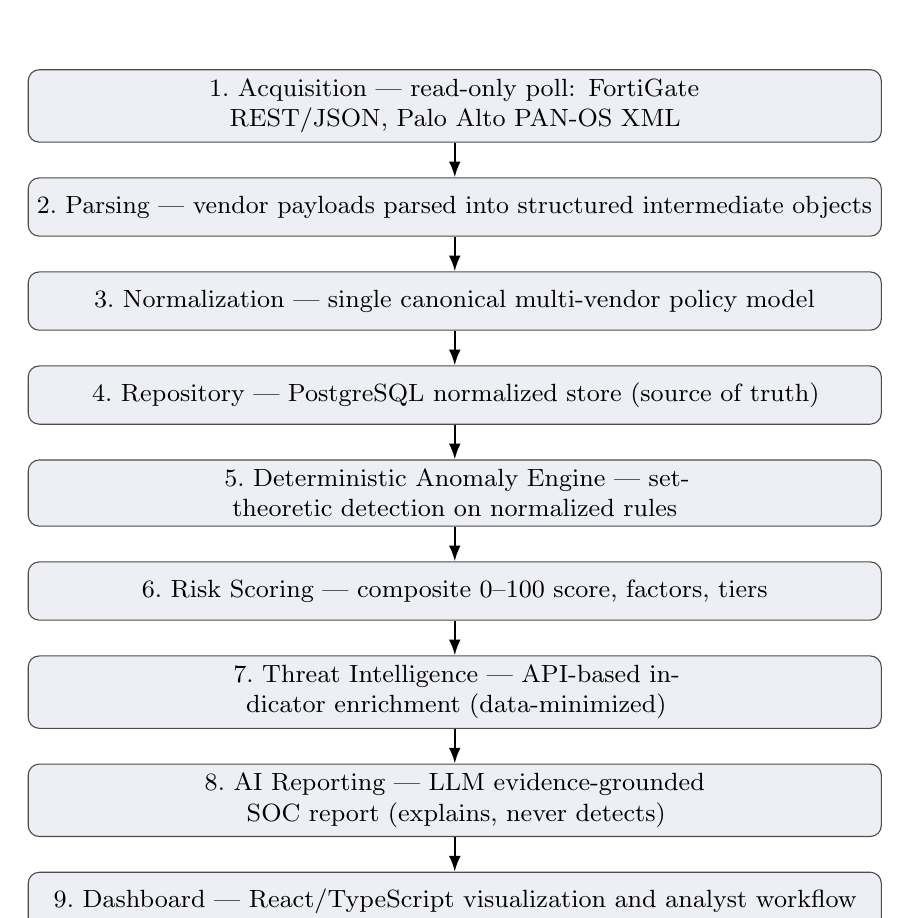
\begin{tikzpicture}[
  stage/.style={draw=black!70, rounded corners, fill=LightGray, text width=10.6cm, align=center, minimum height=7.4mm, font=\small},
  node distance=4.4mm]
\node[stage] (s1) {1.~Acquisition --- read-only poll: FortiGate REST/JSON, Palo Alto PAN-OS XML};
\node[stage, below=of s1] (s2) {2.~Parsing --- vendor payloads parsed into structured intermediate objects};
\node[stage, below=of s2] (s3) {3.~Normalization --- single canonical multi-vendor policy model};
\node[stage, below=of s3] (s4) {4.~Repository --- PostgreSQL normalized store (source of truth)};
\node[stage, below=of s4] (s5) {5.~Deterministic Anomaly Engine --- set-theoretic detection on normalized rules};
\node[stage, below=of s5] (s6) {6.~Risk Scoring --- composite 0--100 score, factors, tiers};
\node[stage, below=of s6] (s7) {7.~Threat Intelligence --- API-based indicator enrichment (data-minimized)};
\node[stage, below=of s7] (s8) {8.~AI Reporting --- LLM evidence-grounded SOC report (explains, never detects)};
\node[stage, below=of s8] (s9) {9.~Dashboard --- React/TypeScript visualization and analyst workflow};
\foreach \a/\b in {s1/s2,s2/s3,s3/s4,s4/s5,s5/s6,s6/s7,s7/s8,s8/s9}
  \draw[-{Latex[length=2mm]}, thick] (\a) -- (\b);
\end{tikzpicture}
\caption{The LuminaFPM end-to-end processing pipeline (nine logical layers).}
\label{fig:pipeline}
\end{figure}

Each conceptual stage in Figure~\ref{fig:pipeline} maps onto a concrete Python package under \texttt{backend/services/} (and, for presentation, onto the React frontend). The stages are as follows.

\begin{enumerate}[leftmargin=2.2em]
  \item \textbf{Acquisition} (\texttt{services/acquisition/}). The only firewall-facing layer, and read-only by construction. A vendor connector (\texttt{FortiGateConnector} or \texttt{PaloAltoConnector}, selected at runtime by \texttt{get\_connector(config)}) authenticates to the device API, polls only read endpoints, and returns an \texttt{AcquisitionBundle} of raw vendor responses. FortiGate is polled over the FortiOS REST API (\texttt{/api/v2/cmdb/firewall/*} and \texttt{/api/v2/monitor/system/status}); Palo Alto is polled over the PAN-OS XML API (\texttt{type=keygen}, \texttt{type=config\&action=show}, \texttt{type=op}). Each raw response is persisted to disk as a \texttt{RawArtifact} with a SHA-256 manifest for replay and audit, and the acquisition job advances through a documented state machine (\texttt{queued} $\rightarrow$ \texttt{running} $\rightarrow$ \texttt{success}/\texttt{partial\_success}/\texttt{failed}/\dots). Acquisition runs asynchronously on a Celery worker and \emph{never} inside the web-request cycle.
  \item \textbf{Parsing} (\texttt{services/parsing/}). Vendor-aware but anomaly-agnostic. \texttt{parse\_artifacts(\dots)} replays the stored artifacts and converts raw FortiGate JSON or Palo Alto XML into a vendor-tagged \texttt{ParsedDevicePayload} capturing rule name, vendor rule ID, vendor UUID, rule order, zones, source/destination/service objects, action, logging, profile group, schedule, NAT, description, tags, and enabled state. No anomaly logic runs here.
  \item \textbf{Normalization} (\texttt{services/normalization/}). \texttt{normalize\_payloads([payload])} is a pure, database-free function that maps each vendor parser model into one canonical rule/object/service model, mapping vendor actions to canonical ones (\texttt{accept}/\texttt{allow}/\texttt{permit} $\rightarrow$ \texttt{allow}) while preserving the original vendor value for audit, and building the object \emph{correlation model} (vendor-owned objects are preserved, canonical objects sit above them, and mapping tables connect the two). It returns a \texttt{NormalizationResult}.
  \item \textbf{Normalized Policy Repository} (PostgreSQL, Schema~v4). The authoritative source of truth for v1. \texttt{persist\_result(\dots)} performs an idempotent upsert keyed on \texttt{(device\_id, vdom\_vsys, vendor\_uuid)} into tables such as \texttt{policy\_rule}, \texttt{network\_object}, \texttt{normalized\_object}, and \texttt{normalized\_service}. Schema ownership is delegated to Alembic migrations rather than runtime \texttt{create\_all}, so there is no destructive auto-sync.
  \item \textbf{Deterministic Anomaly Engine} (\texttt{services/anomaly/}). \texttt{analyze(result)} consumes a reconstructed \texttt{NormalizationResult} and returns a deterministic \texttt{list[Finding]} with no randomness, no mock data, no LLM, and no network access. Determinism is guaranteed by a fixed detector order, a stable rule sort keyed on \texttt{(device\_id, rule\_order, vendor\_uuid, rule\_name)}, and pairwise iteration via \texttt{itertools.combinations} so that the earlier rule always has the lower order. Findings are written as \texttt{rule\_anomaly} rows tied to one \texttt{AnomalyExecutionLog} run (\texttt{engine\_version = "anomaly-engine/1.0.0"}), each carrying the full evidence contract (type, severity, confidence, description, evidence, recommendation, detection mode, affected and related rules).
  \item \textbf{Risk Scoring} (\texttt{services/risk/}). A separate engine that does \emph{not} replace anomaly detection. \texttt{run\_risk(\dots)} aggregates the findings of each active rule into a 0--100 score and a tier (90--100 Critical, 70--89 High, 40--69 Medium, 1--39 Low, 0 Informational), persisting \texttt{risk\_assessment} rows at both rule and device scope. It is triggered best-effort at the end of each anomaly run; a risk failure must never fail the analysis.
  \item \textbf{API-based CTI} (\texttt{services/cti/}). \texttt{run\_cti(\dots)} extracts indicators (public IPs, FQDNs, firmware/CVEs) from the normalized rules, generates CTI queries via the LLM layer, calls external CTI APIs, correlates the responses back to rules as threat observations, and updates the risk score. CTI is kept distinct from the deterministic anomaly path.
  \item \textbf{AI / LLM Reporting} (\texttt{services/llm/}). A provider abstraction (\texttt{LLMProvider}) with a \texttt{GeminiProvider} default and a deterministic, network-free \texttt{OfflineProvider} fallback. Its role is bounded to CTI query generation, CTI review/summary, and evidence-grounded SOC/executive report generation; the LLM is \emph{never} an anomaly authority.
  \item \textbf{Presentation \& Reporting} (\texttt{frontend/}). A React + TypeScript + Vite single-page application rendering the Dashboard, Device Inventory, Policy Explorer, Anomaly/Risk/CTI/Benchmark Centers, Reports, and a logical-policy graph. The graph represents \emph{configured policy relationships only}, never live runtime traffic.
\end{enumerate}

The stages are wired together by an asynchronous task chain so that slow firewall polling never blocks analysis: a \texttt{POST /api/devices/\{id\}/poll} request returns \texttt{202~Accepted} immediately after enqueuing \texttt{poll\_device}; that task chains \texttt{normalize\_device}; which chains \texttt{run\_anomaly\_analysis}; which finally invokes \texttt{run\_risk}. Each task runs on a dedicated Celery queue (\texttt{acquisition}, \texttt{normalization}, \texttt{analysis}, \texttt{cti}, \texttt{reporting}) brokered by Redis, with PostgreSQL serving both as the operational state store and as the Celery result backend. The frontend then reads results back over read-only endpoints. This pipeline \emph{is} the project methodology: every requirement in Section~\ref{sec:ch3-functional} is traceable to one of these layers.

\section{User Requirements and System Privileges}
\label{sec:ch3-users}

LuminaFPM is an analyst- and auditor-facing decision-support tool. Its primary audience is firewall administrators, SOC engineers, and security auditors, together with the cybersecurity development team. Because the platform never enacts changes on firewalls, all user privileges are fundamentally \emph{read-centric}: even the most privileged role manages \emph{platform} configuration (credentials, settings, integrations) rather than \emph{firewall} configuration. The underlying RBAC model defines fine-grained roles (Platform Admin, Firewall Engineer, SOC Analyst, Auditor, Viewer); for the purposes of system analysis these consolidate into three principal user categories, described below.

\subsection{Security Analyst (Firewall Engineer / SOC Analyst)}
\label{sec:ch3-user-analyst}
The Security Analyst is the day-to-day operator of the platform. This user registers firewall devices, configures their read-only poll credentials, triggers acquisition and analysis runs, and investigates the resulting findings. The analyst browses normalized policies in the Policy Explorer, inspects anomaly findings and their evidence in the Anomaly Center, reviews rule- and device-level risk scores in the Risk Center, examines CTI threat observations, and reads AI-generated SOC reports. The analyst's responsibility is to interpret the platform's evidence and to recommend (but not apply, through the platform) remediations to firewall owners.

\subsection{SOC Lead / Administrator (Platform Admin)}
\label{sec:ch3-user-admin}
The SOC Lead / Administrator superset the analyst's capabilities and additionally owns \emph{platform} administration: managing device credentials (create, rotate, test), configuring integrations (CTI API keys, LLM provider and model selection), managing users and roles, and tuning system settings. This role is the trust anchor for the encrypted credential store and is the only role permitted to alter platform-wide configuration. Crucially, even this role holds no capability to modify a firewall — the read-only mandate applies uniformly.

\subsection{Auditor / Viewer}
\label{sec:ch3-user-auditor}
The Auditor / Viewer is a strictly read-only consumer of evidence. An Auditor reviews historical findings, risk assessments, benchmark results, and reports as audit evidence, relying on the immutable per-run logs (\texttt{anomaly\_execution\_log}, raw-artifact SHA-256 manifests) for traceability; a Viewer sees only dashboards and summary pages. Neither can trigger analysis runs, manage credentials, or alter configuration.

Table~\ref{tab:ch3-privileges} summarizes the responsibilities and privileges of the three categories. A check mark ($\checkmark$) denotes a granted privilege and a cross ($\times$) denotes a denied one.

{\small
\setlength{\tabcolsep}{4pt}
\begin{longtable}{L{6.0cm} C{2.8cm} C{2.8cm} C{2.8cm}}
\caption{User categories, responsibilities, and platform privileges.}\label{tab:ch3-privileges}\\
\hline
\hcell{Privilege / Responsibility} & \hcell{Security Analyst} & \hcell{SOC Lead / Admin} & \hcell{Auditor / Viewer} \\
\hline
\endfirsthead
\hline
\hcell{Privilege / Responsibility} & \hcell{Security Analyst} & \hcell{SOC Lead / Admin} & \hcell{Auditor / Viewer} \\
\hline
\endhead
\hline
\endfoot
\hline
\endlastfoot
\hrow Register / edit firewall devices & $\checkmark$ & $\checkmark$ & $\times$ \\
\altrow Configure read-only poll credentials & $\checkmark$ & $\checkmark$ & $\times$ \\
\hrow Trigger acquisition / analysis runs & $\checkmark$ & $\checkmark$ & $\times$ \\
\altrow Browse normalized policies (Policy Explorer) & $\checkmark$ & $\checkmark$ & $\checkmark$ \\
\hrow View anomaly findings + evidence & $\checkmark$ & $\checkmark$ & $\checkmark$ \\
\altrow View rule / device risk scores & $\checkmark$ & $\checkmark$ & $\checkmark$ \\
\hrow View CTI threat observations & $\checkmark$ & $\checkmark$ & $\checkmark$ \\
\altrow Read AI-generated SOC reports & $\checkmark$ & $\checkmark$ & $\checkmark$ \\
\hrow View benchmark results / dashboards & $\checkmark$ & $\checkmark$ & $\checkmark$ \\
\altrow Rotate / test device credentials & $\times$ & $\checkmark$ & $\times$ \\
\hrow Manage CTI / LLM integrations & $\times$ & $\checkmark$ & $\times$ \\
\altrow Manage users, roles, system settings & $\times$ & $\checkmark$ & $\times$ \\
\hrow Modify firewall configuration (any kind) & $\times$ & $\times$ & $\times$ \\
\end{longtable}
}

\section{Assumptions, Constraints, Limitations, and Dependencies}
\label{sec:ch3-acld}

\subsection{Assumptions}
\label{sec:ch3-assumptions}
The analysis assumes that each managed firewall exposes a reachable management API (FortiOS REST for FortiGate, PAN-OS XML for Palo Alto) and that a \emph{dedicated, least-privilege, read-only} API account is provisioned on the device for LuminaFPM to use. It assumes that the network objects and services referenced by the rule base (address objects, service objects, zones) already exist on the device, so that normalization can resolve rule references. It assumes that the operator deploys the supporting infrastructure (PostgreSQL, Redis, the Celery worker) as specified by the Docker Compose stack, and that an encryption key (\texttt{ENCRYPTION\_KEY}) is configured so that stored credentials can be encrypted and later decrypted. Finally, it assumes that human operators, not the platform, carry out any remediation on the firewalls.

\subsection{Constraints}
\label{sec:ch3-constraints}
The dominant constraint is the \textbf{strict read-only mandate}: the platform must never modify, push, delete, reorder, enable, disable, or commit firewall configuration, and no write/commit code path exists in any connector. A second hard constraint is the \textbf{normalized-only analysis rule}: the anomaly engine must analyze normalized records only and must never read raw vendor JSON/XML. The v1 \textbf{vendor scope} is constrained to Fortinet FortiGate and Palo Alto PAN-OS only. The \textbf{datastore} is constrained to PostgreSQL as the single authoritative source of truth (MongoDB is explicitly excluded). Acquisition is constrained to run \textbf{asynchronously} on Celery workers and never inside the FastAPI request cycle. Security constraints further require that device credentials be encrypted at rest with Fernet, never hardcoded, never committed to source control, never exposed to the frontend, and never written to logs (a secret-redacting log filter enforces the last point).

\subsection{Limitations}
\label{sec:ch3-limitations}
Several limitations are deliberate v1 scope boundaries rather than defects, and are stated plainly. First, although the formal anomaly taxonomy enumerates 46 categories, v1 ships the \emph{config-only core}: 14 deterministic detectors (plus one CTI-driven \texttt{threat\_exposure} finding) are implemented, all emitting \texttt{detection\_mode = "config\_only"}; runtime-dependent modes (\texttt{conditional}, \texttt{simulated}, \texttt{future\_enhanced}) are defined in the schema but not yet emitted, because v1 has no live telemetry. Second, the platform performs \emph{no live traffic analysis} — no NetFlow, packet capture, session analysis, or deep packet inspection — and the policy graph therefore represents logical, configured intent only, never observed packet forwarding. Third, the dark-web / LTI subsystem is present in the codebase but disabled by default and treated as optional future research. Fourth, the Docker Compose deployment runs a single Celery worker that drains all routed queues; the specification's recommended horizontal split into per-queue workers is not yet provisioned. Fifth, the backend \texttt{requirements.txt} is unpinned, which is a build-reproducibility caveat worth noting for formal documentation.

\subsection{Dependencies}
\label{sec:ch3-dependencies}
LuminaFPM depends on a Python~3.11 / FastAPI backend, a Celery worker pool, Redis (Celery broker), and PostgreSQL~16 (operational store and Celery result backend), all orchestrated by Docker Compose. The backend depends on \texttt{requests} for FortiGate REST calls and \texttt{defusedxml} for hardened PAN-OS XML parsing, on \texttt{cryptography} (Fernet) for credential encryption, and on a multi-provider LLM stack (Google Gemini SDK by default, with offline fallback). The frontend depends on React~19, React~Router~7, Vite, Recharts, and the Cytoscape graph stack. Externally, the platform depends on the managed firewalls' management APIs being reachable, on third-party CTI API services when CTI is enabled, and on the configured LLM provider's API when online reporting is used (the offline provider removes this dependency for deterministic, network-free reports).

\section{Intended Technologies}
\label{sec:ch3-technologies}

The technology stack is determined directly by the dependency manifests --- \path{backend/requirements.txt}, \path{frontend/package.json}, and \path{docker-compose.yml} --- and by the build images \path{backend/Dockerfile} (\texttt{python:3.11-slim}) and \path{frontend/Dockerfile} (\texttt{node:22-slim}). Backend dependencies are unpinned (resolved at image-build time); frontend dependencies are pinned with caret ranges. Table~\ref{tab:ch3-techstack} maps each architectural layer to the technologies that realize it and the role each plays.

{\small
\setlength{\tabcolsep}{4pt}
\begin{longtable}{L{2.8cm} L{5.4cm} L{6.4cm}}
\caption{Intended technology stack by architectural layer.}\label{tab:ch3-techstack}\\
\hline
\hcell{Layer} & \hcell{Technology} & \hcell{Role} \\
\hline
\endfirsthead
\hline
\hcell{Layer} & \hcell{Technology} & \hcell{Role} \\
\hline
\endhead
\hline
\endfoot
\hline
\endlastfoot
\hrow API / web framework & FastAPI + Uvicorn (ASGI) & REST API surface (routers, dependency injection, OpenAPI); served by Uvicorn. \\
\altrow Data access / ORM & SQLAlchemy + Alembic & ORM models and sessions; schema owned by Alembic migrations (no runtime \texttt{create\_all}). \\
\hrow Validation / config & Pydantic + pydantic-settings & Request/response schemas, normalized-model validation, typed env configuration. \\
\hrow Database & PostgreSQL 16 & Single authoritative source of truth (Schema v4); Celery result backend. \\
\altrow Task queue & Celery (\texttt{celery[redis]}) & Async acquisition / normalization / analysis / CTI / reporting jobs on routed queues. \\
\hrow Broker / cache & Redis 7 & Celery broker and SSE Pub/Sub transport. \\
\altrow Firewall acquisition & \texttt{requests} (FortiOS REST/JSON) & Read-only HTTP client for FortiGate \texttt{cmdb}/\texttt{monitor} GET endpoints. \\
\hrow Firewall acquisition & \texttt{defusedxml} (PAN-OS XML) & Hardened XML parsing of Palo Alto \texttt{keygen}/\texttt{config show}/\texttt{op} responses. \\
\altrow Credential security & \texttt{cryptography} (Fernet) & AES-128-CBC + HMAC encryption of device secrets at rest. \\
\hrow LLM / AI & \texttt{google-generativeai} (Gemini) + LangChain bindings & Default LLM provider for CTI query/review and SOC reporting; offline fallback for deterministic output. \\
\altrow Streaming & \texttt{sse-starlette} & Server-Sent Events for streaming progress / LLM tokens to the UI. \\
\hrow Frontend framework & React 19 + TypeScript + Vite & Single-page dashboard application; Vite dev server and build tool. \\
\altrow Routing & React Router 7 & Client-side routing across the Centers. \\
\hrow Charts / graph & Recharts + Cytoscape (\texttt{cytoscape-dagre}, \texttt{react-cytoscapejs}) & Dashboard charts and the logical-policy graph view. \\
\altrow Styling / icons & Tailwind CSS 4 + \texttt{lucide-react} & Utility-first styling and icon set. \\
\hrow Orchestration & Docker Compose + Nginx & Multi-service deployment; Nginx prepared for production static serving. \\
\end{longtable}
}

\section{Functional Requirements}
\label{sec:ch3-functional}

The functional requirements (FRs) below define the behaviours the platform must exhibit. They are organized by pipeline layer and prioritized as \emph{Must} (mandatory for v1), \emph{Should} (important but degradable), or \emph{Could} (desirable / future-leaning). Each FR is traceable to a layer described in Section~\ref{sec:ch3-methodology}. Table~\ref{tab:ch3-fr} enumerates FR-01 through FR-27.

\begin{longtable}{C{0.08\textwidth} L{0.70\textwidth} C{0.12\textwidth}}
\caption{Functional requirements (FR-01 -- FR-27).}\label{tab:ch3-fr}\\
\hline
\hcell{ID} & \hcell{Requirement} & \hcell{Priority} \\
\hline
\endfirsthead
\hline
\hcell{ID} & \hcell{Requirement} & \hcell{Priority} \\
\hline
\endhead
\hline
\endfoot
\hline
\endlastfoot
\hrow FR-01 & The system shall acquire firewall configuration from FortiGate over the FortiOS REST/JSON API using read-only endpoints only. & Must \\
\altrow FR-02 & The system shall acquire firewall configuration from Palo Alto over the PAN-OS XML API (\texttt{keygen}, \texttt{config show}, \texttt{op}) using read-only operations only. & Must \\
\hrow FR-03 & The system shall persist each raw vendor response as a \texttt{RawArtifact} on disk with a SHA-256 manifest, and record artifact metadata in the database for replay and audit. & Must \\
\altrow FR-04 & The system shall run all acquisition asynchronously on Celery workers and never inside the FastAPI request cycle, returning \texttt{202~Accepted} with a job identifier. & Must \\
\hrow FR-05 & The system shall track each acquisition job through a defined lifecycle (queued, running, success, partial\_success, failed, and error sub-states). & Must \\
\altrow FR-06 & The system shall parse raw FortiGate JSON and Palo Alto XML into vendor-tagged parser models without performing any anomaly logic. & Must \\
\hrow FR-07 & The system shall normalize vendor parser models into a single canonical rule/object/service model, mapping vendor actions to canonical actions while preserving original vendor values. & Must \\
\altrow FR-08 & The system shall build an object correlation model that preserves vendor-owned objects and links them to canonical objects via mapping tables. & Must \\
\hrow FR-09 & The system shall persist normalized data idempotently into PostgreSQL keyed on \texttt{(device\_id, vdom\_vsys, vendor\_uuid)}, supporting incremental re-synchronization. & Must \\
\altrow FR-10 & The system shall run the deterministic anomaly engine over the normalized repository only, never over raw vendor data. & Must \\
\hrow FR-11 & The system shall detect single-rule anomalies including over-permissive rules, any-to-sensitive access, unprotected allows, wide port ranges, missing logging, missing descriptions, disabled-rule review, and object sprawl. & Must \\
\altrow FR-12 & The system shall detect intra-device pairwise anomalies including shadowing, redundancy, duplicate rules, and conflicts. & Must \\
\hrow FR-13 & The system shall produce deterministic, repeatable findings with a fixed detector order and a stable rule sort (no randomness, network, or LLM in the engine). & Must \\
\altrow FR-14 & Every finding shall carry a full evidence contract: anomaly type, severity, confidence, description, evidence facts, recommendation, detection mode, and affected/related rules. & Must \\
\hrow FR-15 & The system shall detect cross-device anomalies (cross-device inconsistency and cross-device security-posture inconsistency) by analyzing all devices together. & Must \\
\altrow FR-16 & The system shall compute a 0--100 risk score and tier (Critical/High/Medium/Low/Informational) per rule and per device, persisting \texttt{risk\_assessment} rows while retaining cross-run history. & Must \\
\hrow FR-17 & The system shall trigger risk scoring best-effort at the end of each anomaly run such that a risk failure never fails the analysis. & Must \\
\altrow FR-18 & The system shall extract indicators (public IPs, FQDNs, firmware/CVEs) and enrich them via external CTI APIs, correlating threat observations back to rules. & Should \\
\hrow FR-19 & The system shall update risk scores from CTI verdicts and label CTI-derived findings with \texttt{detection\_mode = "cti"}. & Should \\
\altrow FR-20 & The system shall generate AI-assisted, evidence-grounded SOC/executive reports and CTI queries via a provider abstraction, with a deterministic offline fallback. & Should \\
\hrow FR-21 & The LLM layer shall never act as an anomaly authority; AI output is bounded to query generation, CTI review, and reporting. & Must \\
\altrow FR-22 & The system shall provide a benchmark framework that scores engine findings against documented ground truth (precision, recall, F1) as an acceptance gate. & Should \\
\hrow FR-23 & The system shall expose read-only REST endpoints for jobs, devices, normalized rules/objects, anomalies, risk, CTI, benchmark, and reports. & Must \\
\altrow FR-24 & The system shall present a React dashboard with Policy Explorer and Anomaly/Risk/CTI/Benchmark Centers plus a logical-policy graph that never depicts live traffic. & Must \\
\hrow FR-25 & The system shall allow operators to create, rotate, and test device credentials, returning status only and never exposing secrets to the frontend. & Must \\
\altrow FR-26 & The system shall never write, push, delete, reorder, enable, disable, or commit any firewall configuration (strict read-only enforcement). & Must \\
\hrow FR-27 & The system shall negotiate transport scheme per device (HTTPS by default; HTTP only for explicitly configured lab hosts) while keeping all requests read-only. & Should \\
\end{longtable}

\section{Non-Functional Requirements}
\label{sec:ch3-nonfunctional}

The non-functional requirements (NFRs) constrain \emph{how well} the platform must satisfy its functional behaviours. They are grouped by quality attribute below and summarized in Table~\ref{tab:ch3-nfr}.

\subsection{Security}
\label{sec:ch3-nfr-security}
Security is the platform's defining quality attribute. The read-only mandate is a security control as much as a functional one: by holding only read-only poll keys and containing no write code path, even a compromised LuminaFPM instance cannot alter a firewall. Device secrets are encrypted at rest with Fernet (AES-128-CBC + HMAC), decrypted only in backend/worker memory, never returned to the frontend, and never logged — a secret-redacting log filter masks API keys, tokens, passwords, and bearer headers. CORS is a restricted allowlist (wildcard-with-credentials is rejected), and PostgreSQL and Redis are not published to the host (internal Docker network only).

\subsection{Reliability and Availability}
\label{sec:ch3-nfr-reliability}
The asynchronous pipeline is tuned for crash-safety: Celery uses late acknowledgement (\texttt{task\_acks\_late}) so a task is acknowledged only after completion, a prefetch multiplier of one to avoid greedy prefetch, and PostgreSQL as a durable result backend. Acquisition tolerates partial failure (\texttt{partial\_success}) when an optional endpoint fails, and risk scoring is best-effort so it cannot fail an analysis run. The job state machine and immutable per-run logs make failures observable and recoverable.

\subsection{Performance}
\label{sec:ch3-nfr-performance}
Per-job-type queue routing ensures slow firewall polling never blocks analysis, CTI, or reporting. The anomaly engine is purely in-memory over the normalized model and uses stable sorting and pairwise combinations, giving predictable, deterministic runtimes. The threat-intel scan path enforces hard and soft time limits (1800\,s / 1500\,s) to bound worst-case execution.

\subsection{Maintainability and Extensibility}
\label{sec:ch3-nfr-maintainability}
The strict layering and the connector/parser registry pattern make the system extensible: a new vendor is added by implementing a connector and a parser behind the existing interfaces, without touching the analytical core. Schema evolution is managed by Alembic migrations. The LLM and CTI providers sit behind abstractions (\texttt{LLMProvider}, \texttt{CTIProvider}), allowing providers to be swapped via configuration.

\subsection{Usability}
\label{sec:ch3-nfr-usability}
Findings are explainable by construction: every finding carries the concrete evidence that produced it and a remediation recommendation, so analysts can act on results without re-deriving them. The dashboard organizes work into purpose-built Centers, and the logical-policy graph is clearly labelled as configured intent rather than live traffic to avoid misinterpretation.

\subsection{Portability}
\label{sec:ch3-nfr-portability}
The entire stack is containerized via Docker Compose and built from standard base images (\texttt{python:3.11-slim}, \texttt{node:22-slim}), so it can be reproduced on any Docker-capable host. Device-local state (the \texttt{.env} file, the \texttt{postgres\_data} volume, and the lab network) is documented as non-transferable, and the credential-encryption key derivation tolerates either a pre-generated Fernet key or a passphrase.

\begin{longtable}{C{1.1cm} L{3.0cm} L{10.1cm}}
\caption{Non-functional requirements summary.}\label{tab:ch3-nfr}\\
\hline
\hcell{ID} & \hcell{Attribute} & \hcell{Requirement} \\
\hline
\endfirsthead
\hline
\hcell{ID} & \hcell{Attribute} & \hcell{Requirement} \\
\hline
\endhead
\hline
\endfoot
\hline
\endlastfoot
\hrow NFR-01 & Security & The platform shall be strictly read-only and shall hold no firewall write capability anywhere in its trust boundary. \\
\altrow NFR-02 & Security & Device credentials shall be encrypted at rest (Fernet), decrypted only in memory, and never exposed to the frontend or logs. \\
\hrow NFR-03 & Security & The API shall enforce a CORS allowlist and shall not publish the database or cache to the host network. \\
\altrow NFR-04 & Reliability & Tasks shall acknowledge only after completion and persist results durably so that worker crashes do not lose work. \\
\hrow NFR-05 & Reliability & Acquisition shall degrade gracefully to partial success, and risk scoring shall never fail an analysis run. \\
\altrow NFR-06 & Performance & Firewall polling shall not block analysis, CTI, or reporting, via per-job-type queue routing. \\
\hrow NFR-07 & Performance & The anomaly engine shall be deterministic and in-memory, with bounded, repeatable runtimes. \\
\altrow NFR-08 & Maintainability & New vendors shall be addable via connector/parser extensions without modifying the anomaly engine. \\
\hrow NFR-09 & Maintainability & Database schema changes shall be managed exclusively through Alembic migrations. \\
\altrow NFR-10 & Usability & Every finding shall be explainable, carrying evidence facts and a remediation recommendation. \\
\hrow NFR-11 & Portability & The full stack shall be reproducible via Docker Compose on any Docker-capable host. \\
\end{longtable}

\section{Virtual Environment and Laboratory Topology}
\label{sec:ch3-lab}

LuminaFPM was developed and validated against a controlled, parallel, shared-network \textbf{VMware laboratory} that hosts both v1 firewalls. The lab follows the \emph{Hybrid Parallel Shared-Network} model: the FortiGate and the Palo Alto firewall both connect to the same logical subnets but operate as \textbf{independent policy engines} — they are not inline, and no production traffic is routed from one through the other. This model is deliberately chosen because it is the cleanest environment for controlled cross-vendor anomaly detection under \emph{identical} logical network conditions: it avoids unnecessary routing complexity, supports clean API extraction from each device, and enables benchmark-driven evaluation of the deterministic engine. The lab is primarily a controlled anomaly-\emph{generation} environment, not a realistic enterprise routing simulation. Figure~\ref{fig:labtopo} shows the topology, its subnets, and the device IP plan.

\begin{figure}[htbp]
\centering
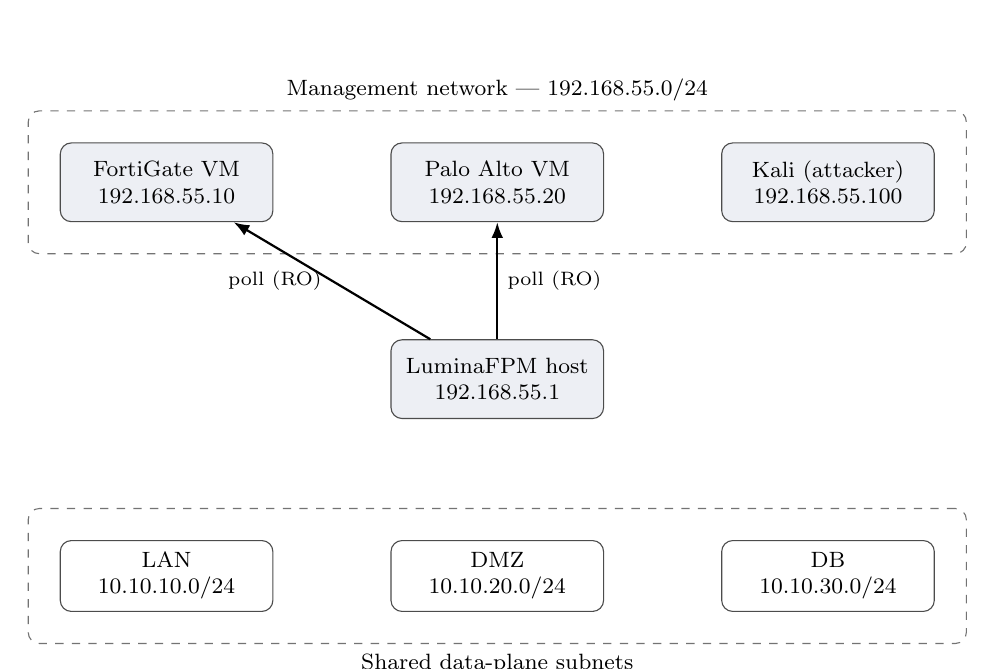
\begin{tikzpicture}[
  dev/.style={draw=black!70, rounded corners, fill=LightGray, align=center, minimum width=2.7cm, minimum height=10mm, font=\footnotesize},
  sub/.style={draw=black!70, rounded corners, fill=white, align=center, minimum width=2.7cm, minimum height=9mm, font=\footnotesize},
  net/.style={draw=black!55, dashed, rounded corners, inner sep=4mm}]
\node[dev] (fgt)  at (0,0)    {FortiGate VM\\192.168.55.10};
\node[dev] (pa)   at (4.2,0)  {Palo Alto VM\\192.168.55.20};
\node[dev] (kali) at (8.4,0)  {Kali (attacker)\\192.168.55.100};
\node[dev] (lum)  at (4.2,-2.5) {LuminaFPM host\\192.168.55.1};
\node[sub] (lan)  at (0,-5.0)  {LAN\\10.10.10.0/24};
\node[sub] (dmz)  at (4.2,-5.0) {DMZ\\10.10.20.0/24};
\node[sub] (db)   at (8.4,-5.0) {DB\\10.10.30.0/24};
\begin{scope}[on background layer]
  \node[net, fit=(fgt)(pa)(kali), label={[font=\footnotesize]above:Management network --- 192.168.55.0/24}] {};
  \node[net, fit=(lan)(dmz)(db), label={[font=\footnotesize]below:Shared data-plane subnets}] {};
\end{scope}
\draw[-{Latex[length=2mm]}, thick] (lum) -- node[left, font=\scriptsize]{poll (RO)} (fgt);
\draw[-{Latex[length=2mm]}, thick] (lum) -- node[right, font=\scriptsize]{poll (RO)} (pa);
\end{tikzpicture}
\caption{Parallel shared-network virtual laboratory topology. LuminaFPM polls both firewalls read-only over the management network; the firewalls independently govern the shared data-plane subnets.}
\label{fig:labtopo}
\end{figure}

\subsection*{Networks and IP plan}
The lab is partitioned into one management/API network and three data-plane subnets:

\begin{itemize}[leftmargin=1.6em]
  \item \textbf{ADMIN/API network} \texttt{192.168.55.0/24} — management and read-only API access. FortiGate management interface is \texttt{192.168.55.10}, Palo Alto management is \texttt{192.168.55.20}, the Kali / API host is \texttt{192.168.55.100}, and the VMware host adapter is \texttt{192.168.55.1}. LuminaFPM reaches both firewalls only over this network.
  \item \textbf{LAN} \texttt{10.10.10.0/24} — internal user network (FortiGate \texttt{port1} \texttt{10.10.10.1}; Palo Alto \texttt{eth1/1} \texttt{10.10.10.2}, zone \texttt{trust}).
  \item \textbf{DMZ} \texttt{10.10.20.0/24} — public-services segment (FortiGate \texttt{port2} \texttt{10.10.20.1}; Palo Alto \texttt{eth1/2} \texttt{10.10.20.2}, zone \texttt{dmz}).
  \item \textbf{DB} \texttt{10.10.30.0/24} — database segment (FortiGate \texttt{port3} \texttt{10.10.30.1}; Palo Alto \texttt{eth1/3} \texttt{10.10.30.2}, zone \texttt{db}).
\end{itemize}

\subsection*{Read-only poll accounts versus the provisioner's write keys}
The lab makes the read-only boundary structural rather than merely procedural by \emph{splitting credentials across trust boundaries}. LuminaFPM is configured with \textbf{read-only poll accounts only} — a dedicated FortiGate read-only API token and a read-only Palo Alto API key (or user/password), stored encrypted in the platform. The \textbf{write-capable admin keys} that build the benchmark rule bases live entirely with the parallel-lab provisioning tooling under \texttt{lab/} (\texttt{provision\_benchmark.py}, \texttt{benchmark\_dataset.py}), \emph{outside} LuminaFPM's trust boundary. That tooling is operator write tooling, not part of the read-only platform; it defaults to \texttt{--dry-run} and requires both \texttt{--apply} and \texttt{--confirm} (plus separate write tokens) to push policy. Consequently, even a fully compromised LuminaFPM instance holds no key capable of altering a firewall. After the provisioner writes the benchmark policy set (13 FortiGate rules and 8 Palo Alto rules with documented expected anomalies and cross-device pairs), LuminaFPM read-syncs the devices and runs the engine; the recorded live lab run covered 2 devices, 20 rules, and 54 findings, with benchmark precision/recall/F1 of 100\% (47/47).

\subsection*{FortiGate-VM constraints}
Two lab-specific FortiGate-VM constraints shaped the implementation. First, the evaluation FortiGate-VM enforces a \textbf{10-policy cap}, which bounds the size of the benchmark rule set that can be provisioned on that device. Second, the FortiGate-VM's HTTPS admin service (\texttt{httpsd}) does not reliably bind port~443 in the lab, so its REST API is \textbf{not reachable over HTTPS}. To accommodate this without weakening production behaviour, acquisition negotiates the transport scheme per device: HTTPS by default, falling back to plain \textbf{HTTP only} for hosts explicitly listed in the \texttt{FIREWALL\_INSECURE\_HTTP\_HOSTS} setting (\texttt{scheme = "http" if device.management\_ip in settings.firewall\_insecure\_http\_hosts else "https"}). This escape hatch applies to FortiGate only — the Palo Alto connector hardcodes HTTPS — and the configuration explicitly warns that it must never be enabled in production, where API tokens would otherwise traverse the network unencrypted.

\section{System Architecture}
\label{sec:ch3-architecture}

LuminaFPM realises the \textit{Hybrid Parallel Shared-Network Architecture} as a strictly layered system in which no layer bypasses the layer beneath it: each layer owns a single responsibility and hands a well-defined, vendor-neutral data structure to the next. The architecture is partitioned, both logically and at runtime, into five concerns: a presentation/API tier, an application/services tier, an asynchronous worker tier, a data/repository tier, and an integration tier that mediates all contact with external systems. Figure~\ref{fig:arch} depicts these tiers and the unidirectional flow of policy intent through them.

\begin{figure}[htbp]
\centering
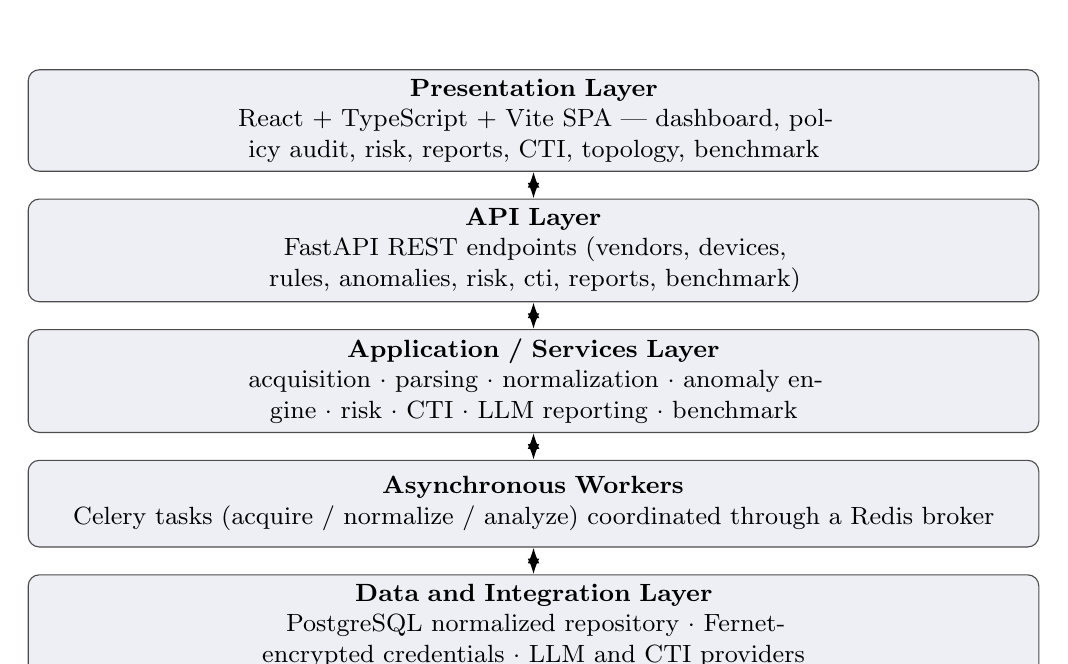
\begin{tikzpicture}[
  layer/.style={draw=black!70, rounded corners, fill=LightGray, text width=12.6cm, align=center, minimum height=11mm, font=\small},
  node distance=3.4mm]
\node[layer] (l1) {\textbf{Presentation Layer}\\React + TypeScript + Vite SPA --- dashboard, policy audit, risk, reports, CTI, topology, benchmark};
\node[layer, below=of l1] (l2) {\textbf{API Layer}\\FastAPI REST endpoints (vendors, devices, rules, anomalies, risk, cti, reports, benchmark)};
\node[layer, below=of l2] (l3) {\textbf{Application / Services Layer}\\acquisition $\cdot$ parsing $\cdot$ normalization $\cdot$ anomaly engine $\cdot$ risk $\cdot$ CTI $\cdot$ LLM reporting $\cdot$ benchmark};
\node[layer, below=of l3] (l4) {\textbf{Asynchronous Workers}\\Celery tasks (acquire / normalize / analyze) coordinated through a Redis broker};
\node[layer, below=of l4] (l5) {\textbf{Data and Integration Layer}\\PostgreSQL normalized repository $\cdot$ Fernet-encrypted credentials $\cdot$ LLM and CTI providers};
\foreach \a/\b in {l1/l2,l2/l3,l3/l4,l4/l5}
  \draw[{Latex[length=2mm]}-{Latex[length=2mm]}, thick] (\a) -- (\b);
\end{tikzpicture}
\caption{Layered system architecture of LuminaFPM.}
\label{fig:arch}
\end{figure}

The \textbf{presentation and API tier} is split across two cooperating processes. The user-facing surface is a React + TypeScript + Vite single-page application (the frontend container) that renders the operational Centers --- Dashboard, Device Inventory, Policy Explorer, Anomaly Center, Risk Center, CTI Threat Center, Benchmark Center, Graph View and Reports --- over a read-only HTTP contract. The server-facing surface is a single FastAPI application (\texttt{backend/main.py}, \texttt{title="LuminaFPM Backend API"}) that mounts one router per resource under the base prefix \texttt{/api/v1}. The API tier performs only fast, transactional work: it validates a request, inserts a job or log row, enqueues a Celery task, and otherwise serves reads from PostgreSQL. A hard architectural rule (Volume~2 \S6.5) forbids any firewall polling inside the web request cycle; consequently every long-running operation returns \texttt{202 Accepted} with a \texttt{job\_id} or \texttt{task\_id} rather than blocking. Cross-Origin Resource Sharing is constrained to a restricted allowlist (\texttt{settings.cors\_allowed\_origins}, default \texttt{http://localhost:5173}); the wildcard-with-credentials combination is explicitly rejected.

The \textbf{application/services tier} is the deterministic core of the platform. It is realised as a set of pure Python packages under \texttt{backend/services/}: acquisition, parsing, normalization, anomaly, risk, cti, llm and benchmark. With the single exception of the acquisition connectors, these services are DB-light or DB-free and contain no I/O against firewalls --- they operate over in-memory model objects (chiefly \texttt{NormalizationResult} and \texttt{Finding}). This purity is deliberate: it makes the analytical pipeline deterministic, unit-testable in isolation, and free of hidden network dependencies.

The \textbf{asynchronous worker tier} executes every operation that is slow, fallible, or contacts an external system. A single Celery application (\texttt{Celery("lumina\_fpm")}) uses Redis as its broker and PostgreSQL as its result backend, with crash-safe tuning (\texttt{task\_acks\_late=True}, \texttt{worker\_prefetch\_multiplier=1}). Work is routed onto per-job-type queues (\texttt{acquisition}, \texttt{normalization}, \texttt{analysis}, \texttt{cti}, \texttt{reporting}) so that slow firewall polling never blocks analysis or reporting. The canonical pipeline chains automatically across these queues: acquisition $\rightarrow$ normalization $\rightarrow$ analysis $\rightarrow$ risk, each stage enqueuing the next on a different queue. Each worker task opens its own SQLAlchemy session because the worker is a distinct process.

The \textbf{data/repository tier} is a single PostgreSQL~16 instance --- the v1 source of truth (ADR-008; MongoDB is explicitly excluded by ADR-021). Its schema (Schema~v4) is owned by Alembic migrations rather than \texttt{Base.metadata.create\_all}, which is deliberately retired from the runtime path so that no destructive auto-synchronisation can occur. The repository holds all normalized policy data, anomaly findings, risk assessments, CTI indicators and observations, benchmark cases and results, and AI reports. The anomaly engine never reads raw vendor output; it consumes only a \texttt{NormalizationResult} reconstructed from this repository by \texttt{normalization.loader.load\_normalized\_result} (ADR-010).

The \textbf{integration tier} encapsulates every boundary crossing. Inward, the acquisition connectors issue read-only requests to the two lab firewalls over the administrative network \texttt{192.168.55.0/24}. Outward, the CTI providers and the LLM provider call third-party HTTP APIs. The read-only mandate (\S\ref{sec:ch3-misuse} and ADR-006) is enforced structurally at this boundary: connectors invoke only GET, \texttt{show}, \texttt{monitor} and \texttt{keygen}/\texttt{op} read endpoints; there is no write, \texttt{set}, \texttt{commit} or \texttt{delete} code path anywhere in the platform. Device secrets are stored encrypted (Fernet) in the \texttt{device\_credential} table and are decrypted only in worker memory, never returned to the frontend and never logged.

\section{Use Case Diagram}
\label{sec:ch3-usecase}

LuminaFPM serves a small set of human actors together with two non-human actors that participate in the platform's automated behaviour. The human actors are distinguished by responsibility rather than by an implemented role-based access-control layer; the route handlers in the current snapshot carry no per-endpoint authorization dependency, so the actor partition below is an \textit{intended} operational model rather than a code-enforced one. Figure~\ref{fig:usecase} summarises the actors and their use cases.

\begin{figure}[htbp]
\centering
\adjustbox{max width=\textwidth,max totalheight=0.88\textheight,center}{%
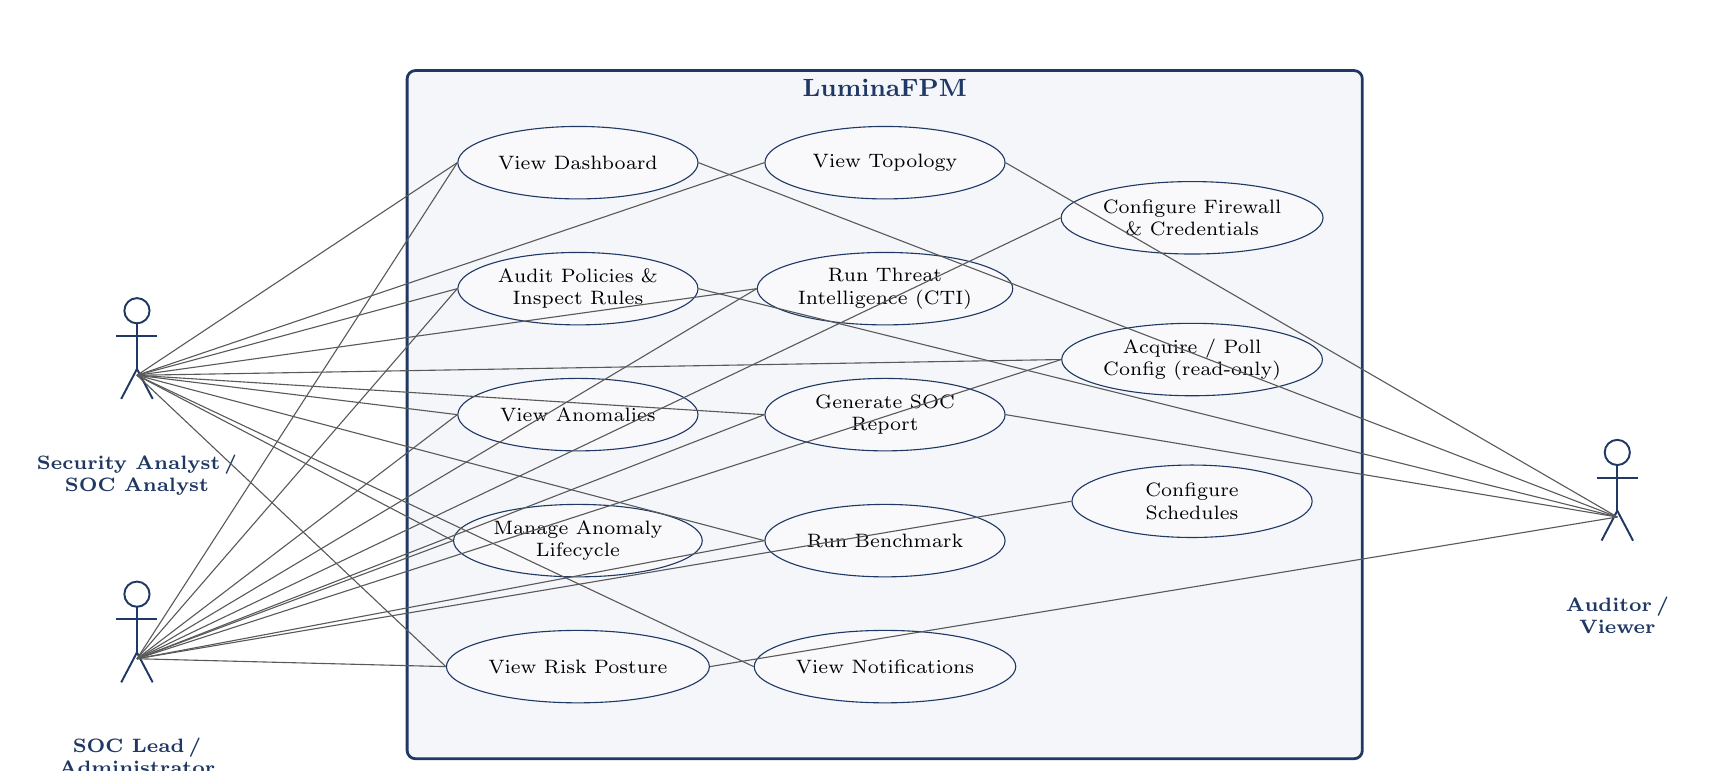
\begin{tikzpicture}[
  >={Stealth[length=2.2mm]},
  actor/.style={
    font=\scriptsize\bfseries, text=NavyBlue, align=center,
    minimum width=2.0cm
  },
  usecase/.style={
    draw=NavyBlue, fill=LightGray!35, ellipse, align=center,
    font=\scriptsize, inner sep=1.2pt, minimum width=3.05cm, minimum height=0.92cm,
    text=black
  },
  assoc/.style={draw=black!65, line width=0.4pt},
]

% ---------- Actors (left and right) ----------
% Stick-figure macro
\newcommand{\stickfigure}[2]{%
  \begin{scope}[shift={(#1)}, draw=NavyBlue, line width=0.7pt]
    \draw (0,0.62) circle (0.16);                 % head
    \draw (0,0.46) -- (0,-0.12);                  % torso
    \draw (-0.26,0.30) -- (0.26,0.30);            % arms
    \draw (0,-0.12) -- (-0.20,-0.50);             % left leg
    \draw (0,-0.12) -- (0.20,-0.50);              % right leg
    \node[actor, anchor=north, yshift=-0.58cm] at (0,-0.50) {#2};
  \end{scope}
}

% Left actors
\stickfigure{0,7.2}{Security Analyst\,/\\SOC Analyst}
\stickfigure{0,3.6}{SOC Lead\,/\\Administrator}
% Right actor
\stickfigure{18.8,5.4}{Auditor\,/\\Viewer}

% ---------- Use cases inside the system boundary (3 columns) ----------
% Column 1 (x = 5.6)
\node[usecase] (uc_dash)   at (5.6,9.7) {View Dashboard};
\node[usecase] (uc_audit)  at (5.6,8.1) {Audit Policies \&\\Inspect Rules};
\node[usecase] (uc_anom)   at (5.6,6.5) {View Anomalies};
\node[usecase] (uc_life)   at (5.6,4.9) {Manage Anomaly\\Lifecycle};
\node[usecase] (uc_risk)   at (5.6,3.3) {View Risk Posture};
% Column 2 (x = 9.5)
\node[usecase] (uc_topo)   at (9.5,9.7) {View Topology};
\node[usecase] (uc_cti)    at (9.5,8.1) {Run Threat\\Intelligence (CTI)};
\node[usecase] (uc_report) at (9.5,6.5) {Generate SOC\\Report};
\node[usecase] (uc_bench)  at (9.5,4.9) {Run Benchmark};
\node[usecase] (uc_notif)  at (9.5,3.3) {View Notifications};
% Column 3 (x = 13.4)
\node[usecase] (uc_cfg)    at (13.4,9.0) {Configure Firewall\\\& Credentials};
\node[usecase] (uc_poll)   at (13.4,7.2) {Acquire / Poll\\Config (read-only)};
\node[usecase] (uc_sched)  at (13.4,5.4) {Configure\\Schedules};

% ---------- System boundary ----------
\begin{scope}[on background layer]
  \node[draw=NavyBlue, line width=1pt, rounded corners=3pt, fill=MidBlue!5,
        fit=(uc_dash)(uc_topo)(uc_cfg)(uc_risk)(uc_notif)(uc_sched),
        inner sep=14pt, inner ysep=20pt] (sysbox) {};
\end{scope}
\node[font=\small\bfseries, text=NavyBlue, anchor=north] at (sysbox.north) {LuminaFPM};

% ---------- Associations ----------
% Security Analyst -> operational use cases
\foreach \t in {uc_dash,uc_audit,uc_anom,uc_life,uc_risk,uc_topo,uc_cti,uc_report,uc_bench,uc_notif,uc_poll}
  \draw[assoc] (0,7.0) -- (\t.west);

% SOC Lead / Administrator -> configure + scheduling (full superset, drawn key extras)
\foreach \t in {uc_cfg,uc_poll,uc_sched,uc_life,uc_audit,uc_anom,uc_report,uc_bench,uc_cti,uc_dash,uc_risk}
  \draw[assoc] (0,3.4) -- (\t.west);

% Auditor / Viewer -> read-only views only
\foreach \t in {uc_dash,uc_audit,uc_risk,uc_report,uc_topo}
  \draw[assoc] (18.8,5.2) -- (\t.east);

\end{tikzpicture}%
}
\caption{Use case diagram of LuminaFPM.}
\label{fig:usecase}
\end{figure}

The \textbf{Security Analyst} is the primary day-to-day actor. The analyst registers FortiGate and Palo Alto devices, configures and tests their encrypted credentials, and triggers a read-only poll of a device. Once the pipeline completes, the analyst browses the normalized Policy Explorer, reviews anomaly findings in the Anomaly Center, inspects the per-rule and per-device risk scores in the Risk Center, examines the CTI Threat Center, requests an evidence-grounded SOC report, and explores the logical policy graph. The analyst also owns the anomaly lifecycle: a finding may be moved from \texttt{open} to \texttt{resolved}, \texttt{suppressed}, \texttt{accepted\_risk} or \texttt{false\_positive}, with a mandatory justification on the suppressing transitions.

The \textbf{SOC Administrator} is a superset actor who, in addition to the analyst's use cases, manages platform-wide configuration: administrator records, device-to-administrator assignments, CTI and LLM provider keys, and the triggering of all-scope (cross-device) analysis runs. The cross-device run is significant because the platform's signature cross-vendor detectors require all devices to be analysed together.

The \textbf{Compliance Auditor} is a read-mostly actor focused on assurance. The auditor consumes the Benchmark Center, where the deterministic engine's output is scored against an authoritative ground-truth matrix (precision, recall, F1, severity-match rate), and reads the immutable history of analysis runs, findings, risk assessments and AI reports. The auditor's principal interest is the platform's explainability and reproducibility guarantee: every finding cites the affected rule, the related rule where applicable, and the concrete evidence that produced it.

Two non-human actors complete the model. The \textbf{Acquisition Scheduler} is the actor on whose behalf jobs may be created without a human request (\texttt{AcquisitionJob.requested\_by} may be \texttt{"scheduler"}); it drives periodic re-polling of devices to keep the normalized repository fresh. The \textbf{LLM / CTI Subsystems} are external-facing actors invoked by the platform: the CTI providers (the always-present offline provider plus optionally AbuseIPDB, OTX or VirusTotal when keyed) supply threat verdicts for extracted indicators, and the LLM provider (Google Gemini by default, with a deterministic offline fallback) generates the SOC and executive reports. The key use cases are enumerated below.

\begin{itemize}[leftmargin=1.4em]
  \item \textbf{Security Analyst:} register/edit device; configure and test credential; trigger device poll; browse normalized policies; review anomalies; inspect rule/device risk; view CTI Threat Center; generate SOC report; explore logical policy graph; manage anomaly lifecycle (resolve / suppress / accept-risk / mark false-positive).
  \item \textbf{SOC Administrator:} all analyst use cases; manage administrators and device assignments; manage provider keys; trigger all-scope cross-device analysis; recalculate risk and CTI.
  \item \textbf{Compliance Auditor:} run and read the benchmark acceptance report; review analysis-run history; read findings, risk and AI reports; verify evidence traceability.
  \item \textbf{Acquisition Scheduler (system actor):} create scheduled acquisition jobs; keep the normalized repository current.
  \item \textbf{LLM / CTI Subsystems (system actors):} enrich indicators with provider verdicts; generate evidence-grounded reports.
\end{itemize}

\section{Misuse Case Diagram}
\label{sec:ch3-misuse}

Because LuminaFPM holds firewall-management credentials and reaches both internal infrastructure and external intelligence APIs, its threat surface is documented through misuse cases: the negative-space counterpart of the use-case model. Each misuse case pairs an abuser goal with the threat actor, the attack vector, and the countermeasure the built system actually implements. Figure~\ref{fig:misuse} overlays these misuse cases on the legitimate actors, and Table~\ref{tab:ch3-misuse} enumerates them.

\begin{figure}[htbp]
\centering
\adjustbox{max width=\textwidth,max totalheight=0.88\textheight,center}{%
\begin{tikzpicture}[
  every node/.style={font=\scriptsize},
  uc/.style={draw=MidBlue!85, very thick, fill=LightGray, ellipse, align=center,
             minimum width=3.0cm, minimum height=1.05cm, inner sep=1pt},
  mc/.style={draw=MisuseRed, very thick, fill=MisuseRed!10, ellipse, align=center,
             minimum width=3.0cm, minimum height=1.05cm, inner sep=1pt, text=MisuseRed!75!black},
  mit/.style={draw=MitGreen, very thick, fill=MitGreen!12, rounded corners, align=center,
              text width=3.0cm, minimum height=1.0cm, inner sep=3pt, text=MitGreen!55!black},
  actor/.style={align=center, font=\scriptsize\bfseries, text=NavyBlue},
  misactor/.style={align=center, font=\scriptsize\bfseries, text=MisuseRed},
  assoc/.style={draw=black!70, thick},
  threatens/.style={draw=MisuseRed, very thick, dashed, -{Latex[length=2.2mm]}},
  mitigates/.style={draw=MitGreen, very thick, dashed, -{Latex[length=2.2mm]}},
  lbl/.style={font=\tiny\itshape, fill=white, inner sep=1pt}]

  % ---- local palette (scoped to this picture) ----
  \definecolor{MisuseRed}{HTML}{B22222}
  \definecolor{MitGreen}{HTML}{2E7D32}

  % ===== legitimate actor (left) =====
  \node[actor] (an) at (-7.6,1.2) {SOC Analyst /\\ Auditor};
  \node[draw=NavyBlue, very thick, circle, minimum size=5mm] (anh) at (-7.6,2.3) {};
  \draw[NavyBlue, very thick] (anh.south) -- ++(0,-0.55)
        (-8.1,1.45) -- (-7.1,1.45)
        (-7.6,0.9) -- ++(-0.4,-0.6) (-7.6,0.9) -- ++(0.4,-0.6);

  % ===== hostile actor (right) =====
  \node[misactor] (att) at (7.6,1.2) {Attacker /\\ Malicious Insider};
  \node[draw=MisuseRed, very thick, circle, minimum size=5mm] (atth) at (7.6,2.3) {};
  \draw[MisuseRed, very thick] (atth.south) -- ++(0,-0.55)
        (7.1,1.45) -- (8.1,1.45)
        (7.6,0.9) -- ++(-0.4,-0.6) (7.6,0.9) -- ++(0.4,-0.6);

  % ===== normal use cases (left column, inside) =====
  \node[uc] (acq)  at (-3.4,3.0)  {Acquire Config\\ (read-only)};
  \node[uc] (view) at (-3.4,1.0)  {View Findings\\ \& Risk};
  \node[uc] (cti)  at (-3.4,-1.0) {Enrich via\\ CTI Providers};
  \node[uc] (rep)  at (-3.4,-3.0) {Generate\\ SOC Report};

  % ===== misuse cases (right column, inside) =====
  \node[mc] (steal) at (3.4,3.4)  {Steal stored\\ credentials};
  \node[mc] (write) at (3.4,1.7)  {Attempt firewall\\ write / commit};
  \node[mc] (xxe)   at (3.4,0.0)  {XML entity-expansion\\ (XXE) injection};
  \node[mc] (exfil) at (3.4,-1.7) {Exfiltrate internal\\ indicators (RFC1918)};
  \node[mc] (secret)at (3.4,-3.4) {Read secrets from\\ logs / errors};

  % ===== mitigation use cases (far-bottom band, green) =====
  \node[mit] (fernet) at (-6.0,-3.0) {Fernet credential\\ encryption};
  \node[mit] (ro)     at (-2.6,-5.0) {Read-only connector\\ contract (no write verbs)};
  \node[mit] (xmlh)   at (1.0,-5.4)  {\texttt{defusedxml}\\ hardened parsing};
  \node[mit] (datam)  at (4.6,-5.0)  {Data-minimization\\ (no RFC1918 sent)};
  \node[mit] (safelog)at (7.6,-3.0)  {Secret-safe\\ logging};

  % ===== system boundary box =====
  \begin{scope}[on background layer]
    \node[draw=NavyBlue, very thick, rounded corners, fill=NavyBlue!4,
          fit=(acq)(rep)(steal)(secret), inner sep=14pt] (sys) {};
  \end{scope}
  \node[anchor=north west, font=\small\bfseries, text=NavyBlue]
        at ([xshift=4pt,yshift=-3pt]sys.north west) {LuminaFPM};

  % ===== actor associations =====
  \draw[assoc] (an.east)  -- (acq.west);
  \draw[assoc] (an.east)  -- (view.west);
  \draw[assoc] (an.east)  -- (cti.west);
  \draw[assoc] (an.east)  -- (rep.west);
  \draw[assoc] (att.west) -- (steal.east);
  \draw[assoc] (att.west) -- (write.east);
  \draw[assoc] (att.west) -- (xxe.east);
  \draw[assoc] (att.west) -- (exfil.east);
  \draw[assoc] (att.west) -- (secret.east);

  % ===== «threatens» (misuse -> normal use case) =====
  \draw[threatens] (steal.west)  -- node[lbl,above]{\guillemotleft threatens\guillemotright} (view.east);
  \draw[threatens] (write.west)  -- node[lbl,above]{\guillemotleft threatens\guillemotright} (acq.east);
  \draw[threatens] (xxe.west)    -- node[lbl,above]{\guillemotleft threatens\guillemotright} (view.east);
  \draw[threatens] (exfil.west)  -- node[lbl,above]{\guillemotleft threatens\guillemotright} (cti.east);
  \draw[threatens] (secret.west) -- node[lbl,below]{\guillemotleft threatens\guillemotright} (rep.east);

  % ===== «mitigates» (mitigation -> misuse case) =====
  \draw[mitigates] (fernet.north)  -- node[lbl,sloped,above]{\guillemotleft mitigates\guillemotright} (steal.south west);
  \draw[mitigates] (ro.north)      -- node[lbl,sloped,above]{\guillemotleft mitigates\guillemotright} (write.south);
  \draw[mitigates] (xmlh.north)    -- node[lbl,sloped,above]{\guillemotleft mitigates\guillemotright} (xxe.south);
  \draw[mitigates] (datam.north)   -- node[lbl,sloped,above]{\guillemotleft mitigates\guillemotright} (exfil.south);
  \draw[mitigates] (safelog.north) -- node[lbl,sloped,above]{\guillemotleft mitigates\guillemotright} (secret.south);

  % ===== legend =====
  \begin{scope}[shift={(-7.9,-4.7)}]
    \node[uc,  minimum width=1.1cm, minimum height=0.55cm] (l1) at (0,0)    {};
    \node[anchor=west, font=\tiny] at (l1.east) {use case};
    \node[mc,  minimum width=1.1cm, minimum height=0.55cm] (l2) at (0,-0.8) {};
    \node[anchor=west, font=\tiny] at (l2.east) {misuse case};
    \node[mit, text width=1.1cm, minimum height=0.5cm] (l3) at (0,-1.7) {};
    \node[anchor=west, font=\tiny] at (l3.east) {mitigation};
  \end{scope}

\end{tikzpicture}%
}
\caption{Misuse case diagram of LuminaFPM.}
\label{fig:misuse}
\end{figure}

{\footnotesize\setlength{\tabcolsep}{4pt}
\begin{xltabular}{\linewidth}{L{3.0cm} L{2.6cm} L{3.8cm} X}
\caption{Misuse cases, threat actors, attack vectors and implemented countermeasures.}
\label{tab:ch3-misuse}\\
\hline
\hcell{Misuse case} & \hcell{Threat actor} & \hcell{Attack vector} & \hcell{Countermeasure (as built)} \\
\hline
\endfirsthead
\hline
\hcell{Misuse case} & \hcell{Threat actor} & \hcell{Attack vector} & \hcell{Countermeasure (as built)} \\
\hline
\endhead
\hline
\endfoot
\hline
\endlastfoot
\hrow
Credential theft & External attacker / malicious insider & Reading stored firewall secrets from the database or API responses to obtain device API keys & Per-device secrets stored as Fernet ciphertext in \texttt{device\_credential.secret\_encrypted}; decrypted only in backend/worker memory via \texttt{credentials.get\_decrypted\_secret}; never serialised to the frontend, never logged; the frontend receives credential \textit{status} only. \\
\altrow
Tampering with the read-only boundary & Malicious insider / compromised platform & Coercing the platform to push, commit, reorder or disable a firewall rule & No write/\texttt{set}/\texttt{commit}/\texttt{delete} code path exists; connectors call only read endpoints (FortiGate \texttt{cmdb}/\texttt{monitor} GETs, PAN-OS \texttt{keygen}/\texttt{config show}/\texttt{op}). Firewall \textit{write} keys live with the lab provisioner, outside Lumina's trust boundary. \\
\hrow
Indicator leakage of RFC1918 space & External CTI provider / network eavesdropper & Exfiltrating internal addressing by submitting private IPs to third-party threat APIs & Data minimisation in \texttt{cti/extract.py}: \texttt{is\_public\_ip} returns \texttt{net.is\_global}, so RFC1918, loopback, link-local and reserved addresses are private; \texttt{extract\_indicators} skips non-public indicators unless \texttt{allow\_internal} is explicitly set; the \texttt{0.0.0.0/0} ANY-sentinel is never an indicator. \\
\altrow
SQL injection & External attacker & Crafted input through API query parameters to subvert repository queries & All persistence flows through SQLAlchemy ORM constructs and parameterised queries; no string-concatenated SQL in the route or service layers; inputs validated by Pydantic schemas. \\
\hrow
LLM prompt injection & Adversarial firewall configuration / external content & Malicious rule descriptions or object names steering the LLM to fabricate findings or remediations & Guardrail system prompt (\texttt{PROMPT\_VERSION="soc-report/2.1"}): the model must use \textit{only} supplied evidence, must not invent CVEs, exploit claims or reputations, and must separate evidence from interpretation. The deterministic engine --- not the LLM --- decides what is an anomaly; the LLM only explains and prioritises. \\
\altrow
Token / secret exposure in transit or logs & Eavesdropper / log reader & Harvesting provider keys or device tokens from logs, error messages or job records & Structured, secret-safe logging (\texttt{core/logging.py}); \texttt{AcquisitionJob.error\_message} stores a safe summary with no secrets; \texttt{db} and \texttt{redis} are bound \texttt{expose}-only on the internal Docker network, not published to the host. \\
\end{xltabular}}

\section{Context Diagram}
\label{sec:ch3-context}

At the highest level of abstraction LuminaFPM is a single process that sits between the firewalls it observes and the people and services that consume its analysis. The context diagram (Figure~\ref{fig:context}) treats the entire platform as one bubble and enumerates the external entities that exchange data with it across the integration boundary.

\begin{figure}[htbp]
\centering
\adjustbox{max width=\textwidth,max totalheight=0.88\textheight,center}{%
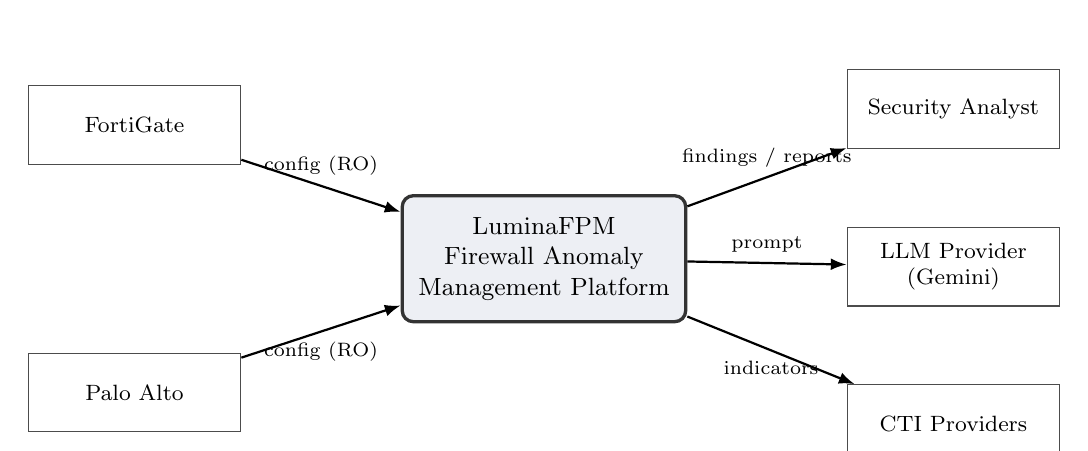
\begin{tikzpicture}[
  sys/.style={draw=black!80, very thick, rounded corners, fill=LightGray, align=center, minimum width=3.6cm, minimum height=1.6cm, font=\small},
  ext/.style={draw=black!70, align=center, minimum width=2.7cm, minimum height=10mm, font=\footnotesize},
  flow/.style={-{Latex[length=2mm]}, thick}]
\node[sys] (s)   at (0,0)     {LuminaFPM\\Firewall Anomaly\\Management Platform};
\node[ext] (fgt) at (-5.2,1.7)  {FortiGate};
\node[ext] (pa)  at (-5.2,-1.7) {Palo Alto};
\node[ext] (an)  at (5.2,1.9)   {Security Analyst};
\node[ext] (llm) at (5.2,-0.1)  {LLM Provider\\(Gemini)};
\node[ext] (cti) at (5.2,-2.1)  {CTI Providers};
\draw[flow] (fgt) -- node[above, font=\scriptsize]{config (RO)} (s);
\draw[flow] (pa)  -- node[below, font=\scriptsize]{config (RO)} (s);
\draw[flow] (s)   -- node[above, font=\scriptsize]{findings / reports} (an);
\draw[flow] (s)   -- node[above, font=\scriptsize]{prompt} (llm);
\draw[flow] (s)   -- node[below, font=\scriptsize]{indicators} (cti);
\end{tikzpicture}
}
\caption{Context diagram: LuminaFPM and its external entities. All firewall interaction is strictly read-only.}
\label{fig:context}
\end{figure}

The two \textbf{firewall devices} are the upstream data sources. The FortiGate device (\texttt{192.168.55.10}) exposes a FortiOS REST/JSON API under \texttt{/api/v2/cmdb/firewall/*} and \texttt{/api/v2/monitor/system/status}; the Palo Alto device (\texttt{192.168.55.20}) exposes the PAN-OS XML API (\texttt{type=keygen}, \texttt{type=config\&action=show}, \texttt{type=op}). Both are contacted strictly read-only, over HTTPS by default and over HTTP only for hosts in the documented lab escape-hatch list. They return raw configuration --- security rules, address and address-group objects, service and service-group objects, and device metadata --- and receive nothing but read requests in return.

The \textbf{Security Analyst} (standing in for the human actors of \S\ref{sec:ch3-usecase}) is the principal downstream consumer: a browser client that drives the platform through the read-only \texttt{/api/v1} contract and receives normalized policies, findings, risk scores, CTI results, reports and the logical graph.

Two classes of third-party service are downstream of the platform's enrichment stages. The \textbf{LLM provider} (Google Gemini at \texttt{generativelanguage.googleapis.com}, with a network-free offline fallback) receives an evidence-grounded prompt and returns generated report prose. The \textbf{CTI providers} (AbuseIPDB at \texttt{api.abuseipdb.com}, optionally OTX and VirusTotal, alongside the always-present offline provider) receive \textit{only public} indicators and return threat verdicts. Both external services are invoked exclusively from the asynchronous worker tier, never from the web request cycle, and both are reached over outbound HTTPS that carries no firewall secrets and no private addressing.

\section{Data Flow Diagram}
\label{sec:ch3-dfd}

The data-flow view decomposes the platform into the six processing stages that transform raw firewall configuration into scored, enriched, narrated intelligence, together with the data stores that persist each intermediate result. Figure~\ref{fig:dfd} shows these processes, the external entities of \S\ref{sec:ch3-context}, and the flows between them.

\begin{figure}[htbp]
\centering
\adjustbox{max width=\textwidth,max totalheight=0.88\textheight,center}{%
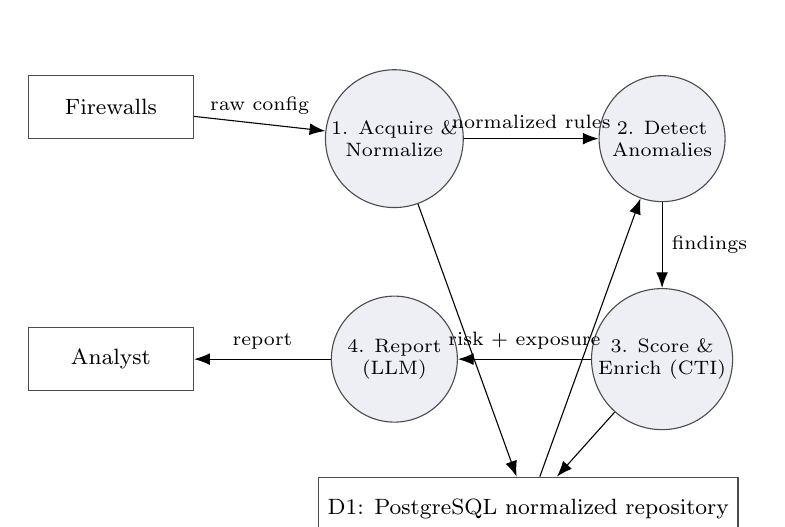
\begin{tikzpicture}[
  proc/.style={draw=black!70, circle, fill=LightGray, align=center, minimum size=1.6cm, font=\scriptsize, inner sep=1pt},
  ent/.style={draw=black!70, align=center, minimum width=2.1cm, minimum height=8mm, font=\footnotesize},
  store/.style={draw=black!70, align=center, minimum width=4.6cm, minimum height=8mm, font=\footnotesize},
  flow/.style={-{Latex[length=2mm]}}]
\node[ent]   (fw) at (-5.2,1)  {Firewalls};
\node[ent]   (an) at (-5.2,-2.2) {Analyst};
\node[proc]  (p1) at (-1.6,0.6) {1. Acquire \&\\Normalize};
\node[proc]  (p2) at (1.8,0.6)  {2. Detect\\Anomalies};
\node[proc]  (p3) at (1.8,-2.2) {3. Score \&\\Enrich (CTI)};
\node[proc]  (p4) at (-1.6,-2.2){4. Report\\(LLM)};
\node[store] (db) at (0.1,-4.1) {D1: PostgreSQL normalized repository};
\draw[flow] (fw) -- node[above,font=\scriptsize]{raw config} (p1);
\draw[flow] (p1) -- node[above,font=\scriptsize]{normalized rules} (p2);
\draw[flow] (p2) -- node[right,font=\scriptsize]{findings} (p3);
\draw[flow] (p3) -- node[above,font=\scriptsize]{risk + exposure} (p4);
\draw[flow] (p4) -- node[above,font=\scriptsize]{report} (an);
\draw[flow] (p1) -- (db);
\draw[flow] (db) -- (p2);
\draw[flow] (p3) -- (db);
\end{tikzpicture}
}
\caption{Data flow diagram of the LuminaFPM analysis pipeline.}
\label{fig:dfd}
\end{figure}

\textbf{Process 1 --- Acquire.} The acquisition connectors authenticate to a firewall, poll its read-only endpoints, and persist each response as a raw artifact on disk under \texttt{/raw\_acquisition/\{vendor\}/\{device\}/\{job\}/} with a SHA-256 manifest. The flow is governed by an \texttt{AcquisitionJob} lifecycle (\texttt{queued} $\rightarrow$ \texttt{running} $\rightarrow$ \texttt{success}/\texttt{partial\_success}/failure states). \textit{Data stores written:} \texttt{acquisition\_job}, \texttt{raw\_artifact} (plus the filesystem artifact store).

\textbf{Process 2 --- Normalize.} The parser replays the stored artifacts into vendor-tagged \texttt{ParsedDevicePayload} objects, and the normalization engine (pure, DB-free) maps them into one canonical model --- canonical actions, canonical objects and services --- while preserving vendor traceability through the correlation-model mapping tables. The thin persist layer performs an idempotent upsert keyed on \texttt{(device\_id, vdom\_vsys, vendor\_uuid)}. \textit{Data stores written:} \texttt{policy\_rule}, \texttt{network\_object}, \texttt{normalized\_object}, \texttt{object\_normalization\_mapping}, \texttt{service\_object}, \texttt{normalized\_service}, \texttt{service\_normalization\_mapping}, \texttt{rule\_object\_mapping}, \texttt{rule\_service\_mapping}.

\textbf{Process 3 --- Detect.} The deterministic anomaly engine reconstructs a \texttt{NormalizationResult} from the repository and runs the fixed-order detector set over it, producing explainable findings (no randomness, no network, no LLM). \textit{Data stores written:} \texttt{anomaly\_execution\_log}, \texttt{rule\_anomaly}.

\textbf{Process 4 --- Score.} The risk scorer aggregates each rule's findings into a 0--100 score with a factor breakdown, then blends the worst rules into a device-level score. \textit{Data store written:} \texttt{risk\_assessment}.

\textbf{Process 5 --- Enrich.} The CTI runner extracts public indicators from the network objects, queries the CTI providers, records the worst verdict per indicator, and correlates malicious indicators back to allow-rules across all devices as \texttt{threat\_exposure} findings, before recomputing risk so the CTI factor lands. \textit{Data stores written:} \texttt{cti\_indicator}, \texttt{cti\_observation}, additional \texttt{rule\_anomaly} (\texttt{detection\_mode="cti"}).

\textbf{Process 6 --- Report.} The LLM reporter assembles an evidence-reference bundle (anomaly IDs, risk ID, CTI observation IDs), calls the provider under the guardrail prompt, and always persists the result. \textit{Data store written:} \texttt{llm\_report}.

A parallel benchmark process reads \texttt{rule\_anomaly} (filtered to \texttt{config\_only} findings) and the ground-truth matrix to write \texttt{benchmark\_case} and \texttt{benchmark\_result}, providing the acceptance gate that the auditor of \S\ref{sec:ch3-usecase} consumes.

\section{Entity Relationship Diagram}
\label{sec:ch3-erd}

The persistence layer is a single relational schema (Schema~v4) defined in \path{backend/models/models.py} and owned by Alembic migrations. Its design embodies the platform's central idea: vendor-owned records are preserved verbatim, a canonical layer sits above them, and explicit mapping tables connect the two so that cross-vendor equivalence is established through normalized correlation keys rather than raw vendor names. Figure~\ref{fig:erd} shows the core entities and their relationships.

\begin{sidewaysfigure}
\centering
\adjustbox{max width=\textheight,max totalheight=\textwidth,center}{%
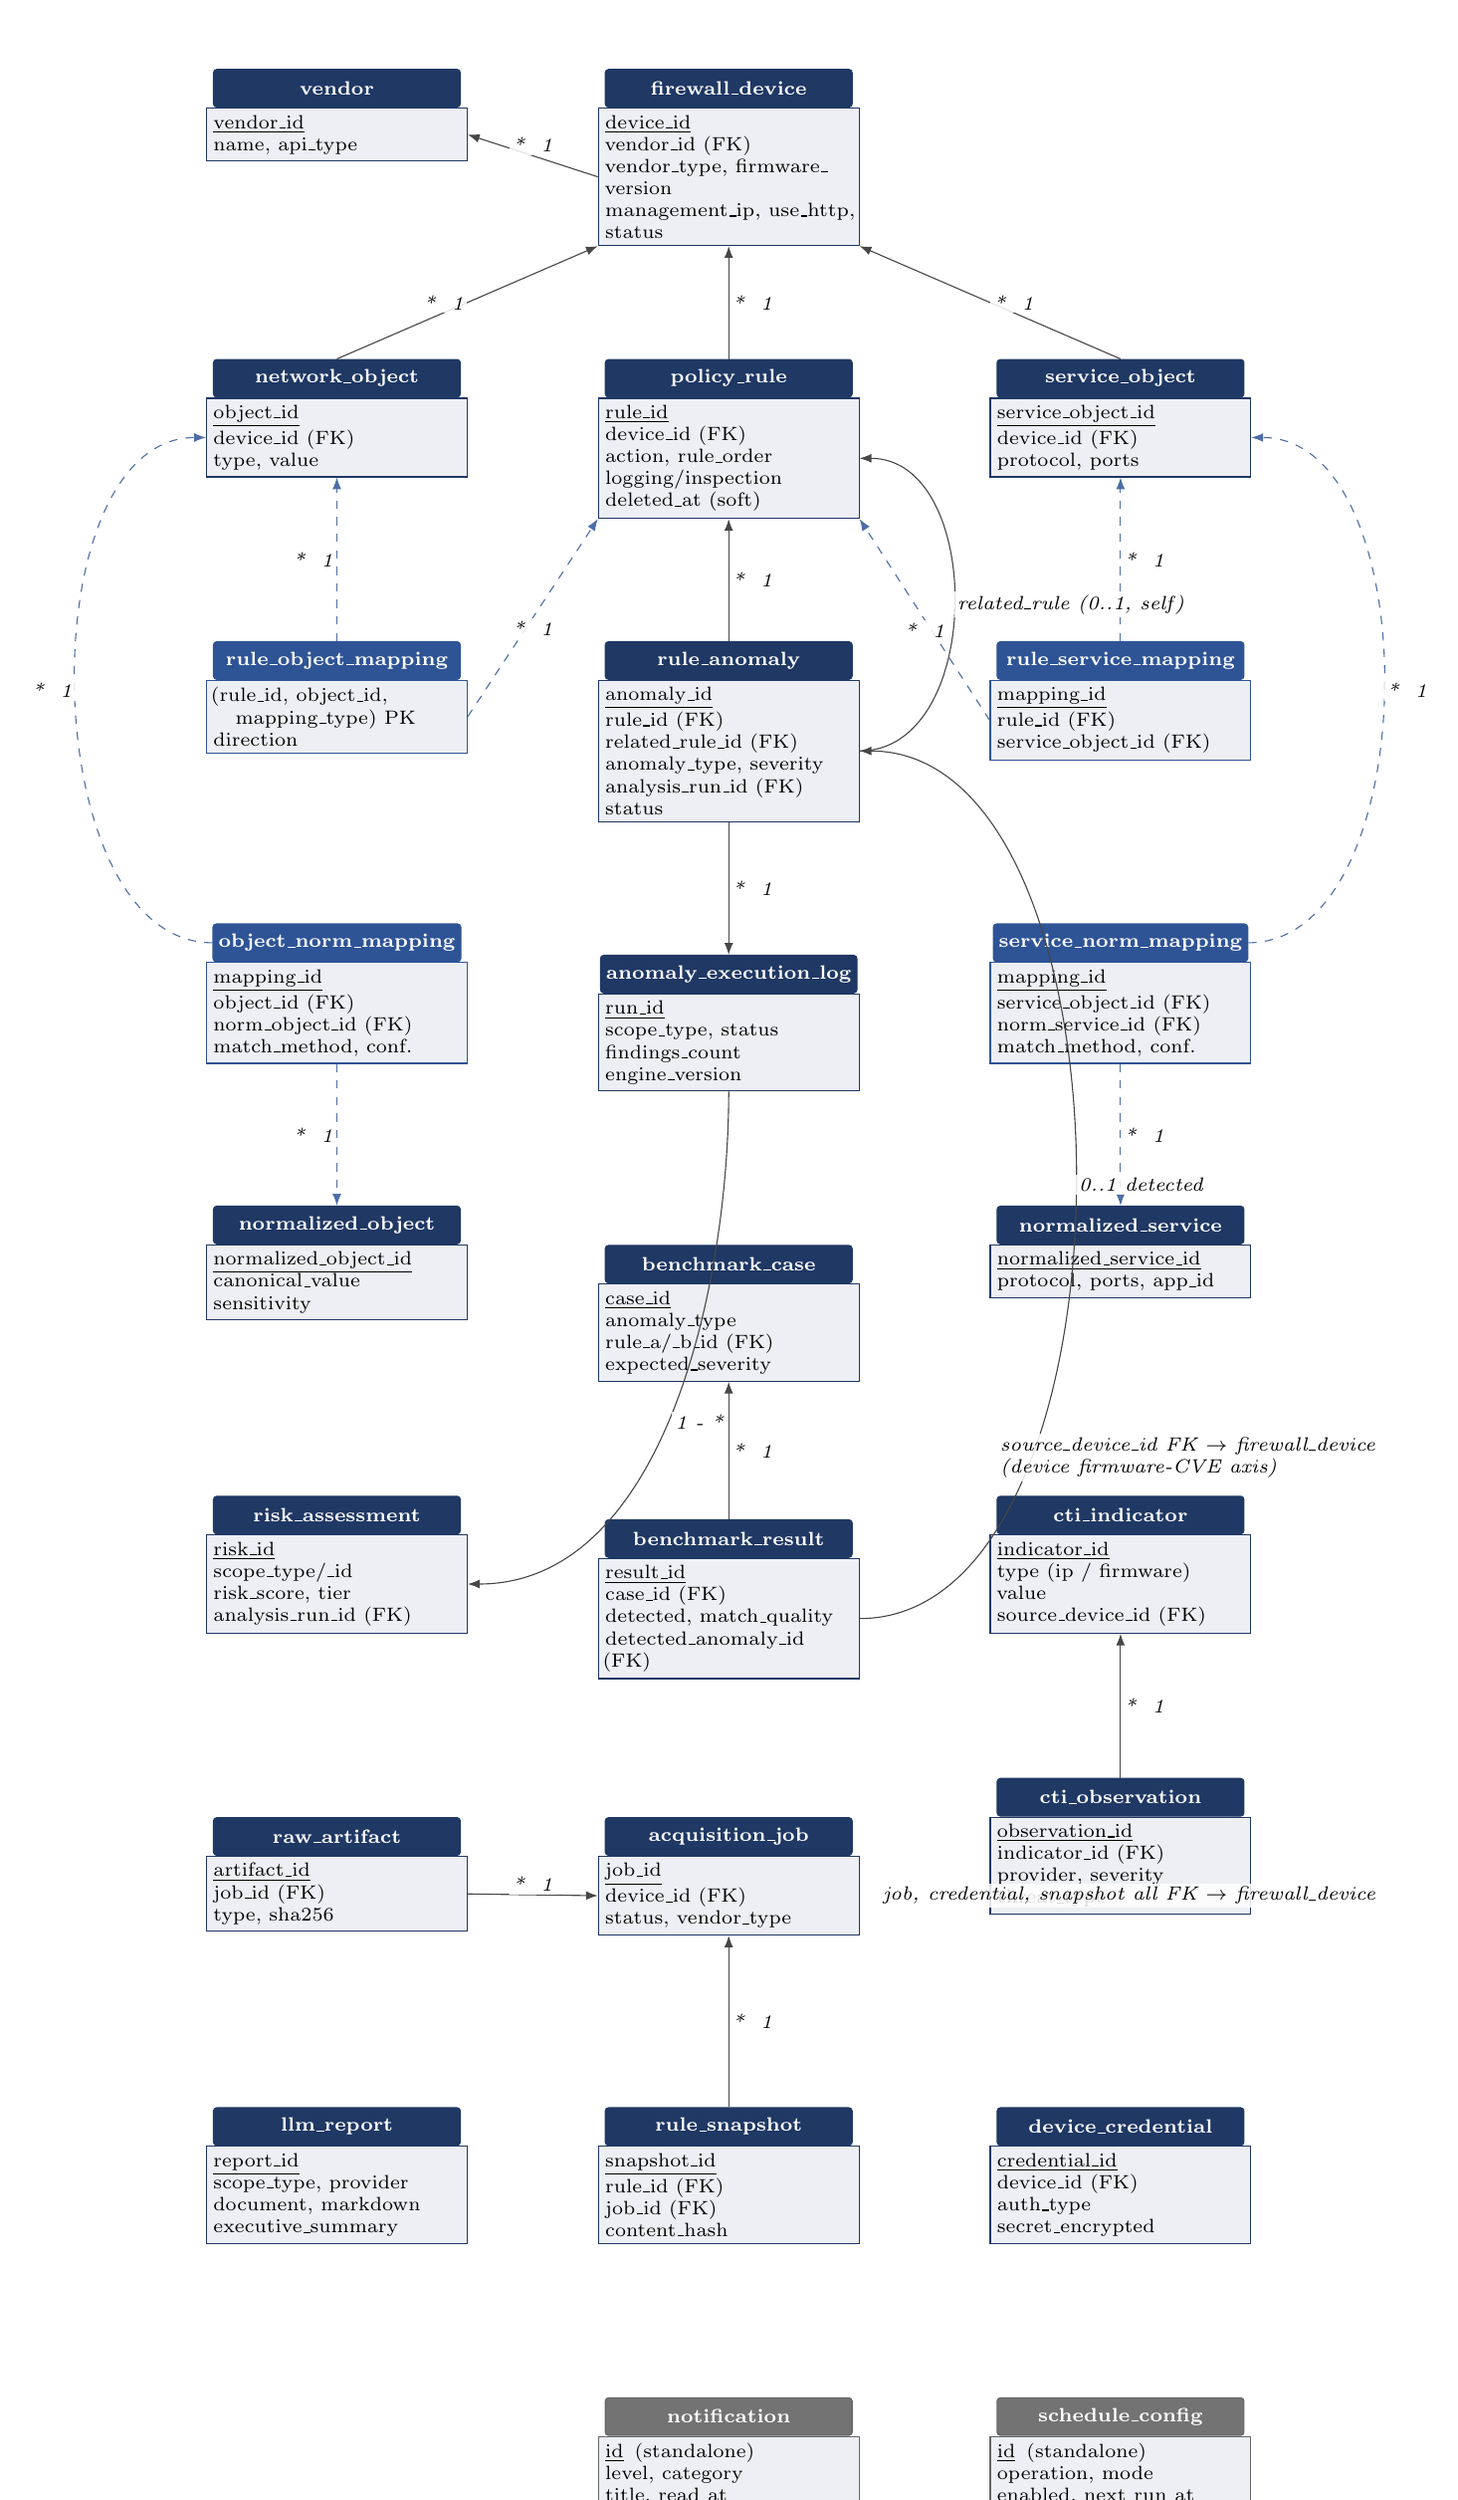
\begin{tikzpicture}[
  font=\scriptsize,
  % ── entity = colored header strip over a body listing a few key columns ──
  ehead/.style={draw=NavyBlue, fill=NavyBlue, text=white, font=\scriptsize\bfseries,
                align=center, minimum width=3.15cm, minimum height=4.8mm,
                inner sep=2pt, rounded corners=1.2pt},
  ebody/.style={draw=NavyBlue, fill=LightGray, text=black, font=\scriptsize,
                align=left, text width=3.15cm, minimum height=4.8mm, inner sep=2.5pt},
  % bridge / association table — MidBlue header to read as a link table
  bhead/.style={draw=MidBlue, fill=MidBlue, text=white, font=\scriptsize\bfseries,
                align=center, minimum width=3.15cm, minimum height=4.8mm,
                inner sep=2pt, rounded corners=1.2pt},
  bbody/.style={draw=MidBlue, fill=LightGray, text=black, font=\scriptsize,
                align=left, text width=3.15cm, minimum height=4.8mm, inner sep=2.5pt},
  % standalone table — gray header (no FK into the core graph)
  shead/.style={draw=black!60, fill=black!55, text=white, font=\scriptsize\bfseries,
                align=center, minimum width=3.15cm, minimum height=4.8mm,
                inner sep=2pt, rounded corners=1.2pt},
  sbody/.style={draw=black!60, fill=LightGray, text=black, font=\scriptsize,
                align=left, text width=3.15cm, minimum height=4.8mm, inner sep=2.5pt},
  rel/.style={font=\scriptsize\itshape, inner sep=1.2pt, fill=white, fill opacity=0.85,
              text opacity=1},
  edge/.style={draw=black!72, -{Latex[length=1.5mm]}},
  link/.style={draw=MidBlue!85, dashed, -{Latex[length=1.5mm]}},
  ]

% ====================  COLUMN x: L=0  C=5  R=10  ====================
% Each entity is a header node with its body placed directly beneath (below=0pt).

% ---------- ownership root (top) ----------
\node[ehead] (venH) at (0,0) {vendor};
\node[ebody,below=0pt of venH] (venB)
  {\underline{vendor\_id}\\name,\ api\_type};

\node[ehead] (devH) at (5,0) {firewall\_device};
\node[ebody,below=0pt of devH] (devB)
  {\underline{device\_id}\\vendor\_id (FK)\\vendor\_type, firmware\_version\\management\_ip, use\_http, status};

% ---------- vendor object / rule / service ----------
\node[ehead] (objH) at (0,-3.7) {network\_object};
\node[ebody,below=0pt of objH] (objB)
  {\underline{object\_id}\\device\_id (FK)\\type,\ value};

\node[ehead] (ruleH) at (5,-3.7) {policy\_rule};
\node[ebody,below=0pt of ruleH] (ruleB)
  {\underline{rule\_id}\\device\_id (FK)\\action, rule\_order\\logging/inspection\\deleted\_at (soft)};

\node[ehead] (svcH) at (10,-3.7) {service\_object};
\node[ebody,below=0pt of svcH] (svcB)
  {\underline{service\_object\_id}\\device\_id (FK)\\protocol,\ ports};

% ---------- rule<->object / rule<->service bridges ----------
\node[bhead] (romH) at (0,-7.3) {rule\_object\_mapping};
\node[bbody,below=0pt of romH] (romB)
  {(rule\_id, object\_id,\\\hspace{1em}mapping\_type) PK\\direction};

\node[bhead] (rsmH) at (10,-7.3) {rule\_service\_mapping};
\node[bbody,below=0pt of rsmH] (rsmB)
  {\underline{mapping\_id}\\rule\_id (FK)\\service\_object\_id (FK)};

% ---------- canonical normalization layer ----------
\node[bhead] (onmH) at (0,-10.9) {object\_norm\_mapping};
\node[bbody,below=0pt of onmH] (onmB)
  {\underline{mapping\_id}\\object\_id (FK)\\norm\_object\_id (FK)\\match\_method, conf.};
\node[ehead] (noH) at (0,-14.5) {normalized\_object};
\node[ebody,below=0pt of noH] (noB)
  {\underline{normalized\_object\_id}\\canonical\_value\\sensitivity};

\node[bhead] (snmH) at (10,-10.9) {service\_norm\_mapping};
\node[bbody,below=0pt of snmH] (snmB)
  {\underline{mapping\_id}\\service\_object\_id (FK)\\norm\_service\_id (FK)\\match\_method, conf.};
\node[ehead] (nsH) at (10,-14.5) {normalized\_service};
\node[ebody,below=0pt of nsH] (nsB)
  {\underline{normalized\_service\_id}\\protocol, ports, app\_id};

% ---------- analysis : anomaly / run ----------
\node[ehead] (anomH) at (5,-7.3) {rule\_anomaly};
\node[ebody,below=0pt of anomH] (anomB)
  {\underline{anomaly\_id}\\rule\_id (FK)\\related\_rule\_id (FK)\\anomaly\_type, severity\\analysis\_run\_id (FK)\\status};

\node[ehead] (runH) at (5,-11.3) {anomaly\_execution\_log};
\node[ebody,below=0pt of runH] (runB)
  {\underline{run\_id}\\scope\_type, status\\findings\_count\\engine\_version};

% ---------- risk (left, under normalization) ----------
\node[ehead] (riskH) at (0,-18.2) {risk\_assessment};
\node[ebody,below=0pt of riskH] (riskB)
  {\underline{risk\_id}\\scope\_type/\_id\\risk\_score, tier\\analysis\_run\_id (FK)};

% ---------- benchmark (center) ----------
\node[ehead] (bcH) at (5,-15.0) {benchmark\_case};
\node[ebody,below=0pt of bcH] (bcB)
  {\underline{case\_id}\\anomaly\_type\\rule\_a/\_b\_id (FK)\\expected\_severity};
\node[ehead] (brH) at (5,-18.5) {benchmark\_result};
\node[ebody,below=0pt of brH] (brB)
  {\underline{result\_id}\\case\_id (FK)\\detected, match\_quality\\detected\_anomaly\_id (FK)};

% ---------- CTI axis (right) ----------
\node[ehead] (ctiH) at (10,-18.2) {cti\_indicator};
\node[ebody,below=0pt of ctiH] (ctiB)
  {\underline{indicator\_id}\\type (ip / firmware)\\value\\source\_device\_id (FK)};
\node[ehead] (obsH) at (10,-21.8) {cti\_observation};
\node[ebody,below=0pt of obsH] (obsB)
  {\underline{observation\_id}\\indicator\_id (FK)\\provider, severity\\threat\_type};

% ---------- acquisition (bottom-left/center) ----------
\node[ehead] (artH) at (0,-22.3) {raw\_artifact};
\node[ebody,below=0pt of artH] (artB)
  {\underline{artifact\_id}\\job\_id (FK)\\type, sha256};
\node[ehead] (jobH) at (5,-22.3) {acquisition\_job};
\node[ebody,below=0pt of jobH] (jobB)
  {\underline{job\_id}\\device\_id (FK)\\status, vendor\_type};
\node[ehead] (snapH) at (5,-26.0) {rule\_snapshot};
\node[ebody,below=0pt of snapH] (snapB)
  {\underline{snapshot\_id}\\rule\_id (FK)\\job\_id (FK)\\content\_hash};

% ---------- reporting + credential ----------
\node[ehead] (repH) at (0,-26.0) {llm\_report};
\node[ebody,below=0pt of repH] (repB)
  {\underline{report\_id}\\scope\_type, provider\\document, markdown\\executive\_summary};
\node[ehead] (credH) at (10,-26.0) {device\_credential};
\node[ebody,below=0pt of credH] (credB)
  {\underline{credential\_id}\\device\_id (FK)\\auth\_type\\secret\_encrypted};

% ---------- standalone NEW tables (gray) ----------
\node[shead] (schedH) at (10,-29.7) {schedule\_config};
\node[sbody,below=0pt of schedH] (schedB)
  {\underline{id}\ \,(standalone)\\operation, mode\\enabled, next\_run\_at};
\node[shead] (notifH) at (5,-29.7) {notification};
\node[sbody,below=0pt of notifH] (notifB)
  {\underline{id}\ \,(standalone)\\level, category\\title, read\_at};

% ============================  RELATIONSHIPS  ============================
% Cardinality convention: "1 --- *" reads parent(1) to child(many); "0..1" optional.

% ownership  (vendor 1 - * device ; device 1 - * rule/object/service)
\draw[edge] (devB.west)  -- node[rel,above]{*\ \ 1} (venB.east);
\draw[edge] (ruleH.north) -- node[rel,right]{*\ \ 1} (devB.south);
\draw[edge] (objH.north)  -- node[rel,left]{*\ \ 1} (devB.south west);
\draw[edge] (svcH.north)  -- node[rel,right]{*\ \ 1} (devB.south east);

% rule <-> object  (M:N via rule_object_mapping)
\draw[link] (romH.north) -- node[rel,left]{*\ \ 1} (objB.south);
\draw[link] (romB.east)  -- node[rel,below]{*\ \ 1} (ruleB.south west);
% rule <-> service (M:N via rule_service_mapping)
\draw[link] (rsmH.north) -- node[rel,right]{*\ \ 1} (svcB.south);
\draw[link] (rsmB.west)  -- node[rel,below]{*\ \ 1} (ruleB.south east);

% canonical normalization bridges  (object/service <-> normalized via mapping)
% object axis: object_normalization_mapping links network_object (above) to
% normalized_object (below). The "up to object" leg routes through the left
% gutter to clear the rule_object_mapping box that sits between them.
\draw[link] (onmH.west) to[out=180,in=180,looseness=0.9]
  node[rel,left]{*\ \ 1} (objB.west);
\draw[link] (onmB.south) -- node[rel,left]{*\ \ 1} (noH.north);
% service axis: symmetric, routed through the right gutter.
\draw[link] (snmH.east) to[out=0,in=0,looseness=0.9]
  node[rel,right]{*\ \ 1} (svcB.east);
\draw[link] (snmB.south) -- node[rel,right]{*\ \ 1} (nsH.north);

% analysis : rule 1 - * anomaly ; self-ref related_rule
\draw[edge] (anomH.north) -- node[rel,right]{*\ \ 1} (ruleB.south);
\draw[edge] (anomB.east) to[out=0,in=0,looseness=1.1]
  node[rel,right]{related\_rule (0..1, self)} (ruleB.east);
% run 1 - * anomaly ; run 1 - * risk
\draw[edge] (anomB.south) -- node[rel,right]{*\ \ 1} (runH.north);
\draw[edge] (runB.south) to[out=-90,in=0,looseness=0.9]
  node[rel,below right]{1 - *} (riskB.east);

% benchmark : case 1 - * result ; result 0..1 anomaly ; case -> rules(anomaly cluster)
\draw[edge] (brH.north) -- node[rel,right]{*\ \ 1} (bcB.south);
\draw[edge] (brB.east) to[out=0,in=0,looseness=0.85]
  node[rel,right]{0..1 detected} (anomB.east);

% CTI : indicator 1 - * observation ; firmware-axis indicator <- device (FK, far above)
\draw[edge] (obsH.north) -- node[rel,right]{*\ \ 1} (ctiB.south);
\node[rel, anchor=south west, align=left] at ($(ctiH.north west)+(0,0.18)$)
  {source\_device\_id FK $\to$ firewall\_device\\(device firmware-CVE axis)};

% acquisition : job 1 - * artifact ; job 1 - * snapshot
\draw[edge] (artB.east) -- node[rel,above]{*\ \ 1} (jobB.west);
\draw[edge] (snapH.north) -- node[rel,right]{*\ \ 1} (jobB.south);
% job * - 1 device  (FK device_id) — short stub annotation, device sits far above
\node[rel, anchor=west] at ($(jobB.east)+(0.25,0)$) {job, credential, snapshot all FK $\to$ firewall\_device};
\end{tikzpicture}}
\caption{Entity--relationship diagram of LuminaFPM Schema~v4. NavyBlue boxes are entities and MidBlue boxes are association (bridge) tables; gray boxes are standalone tables with no foreign key into the core graph. The diagram shows vendor/device ownership; the normalized policy model (the \texttt{policy\_rule}$\leftrightarrow$\texttt{network\_object} and \texttt{policy\_rule}$\leftrightarrow$\texttt{service\_object} bridges, and the canonical normalization layer reached through \texttt{object\_/service\_normalization\_mapping}); the analysis tier (\texttt{rule\_anomaly} with a self-referential \texttt{related\_rule}, the \texttt{anomaly\_execution\_log} run that aggregates anomalies and \texttt{risk\_assessment}); the CTI \texttt{cti\_indicator}/\texttt{cti\_observation} axis (including the device firmware axis); the \texttt{benchmark\_case}/\texttt{benchmark\_result} pair; acquisition (\texttt{acquisition\_job}, \texttt{raw\_artifact}, \texttt{rule\_snapshot}); and reporting (\texttt{llm\_report}), with the standalone \texttt{schedule\_config} and \texttt{notification} tables. Cardinalities are shown as 1 / * (and 0..1 for optional). Dashed edges mark the many-to-many correlations resolved by bridge tables.}
\label{fig:erd}
\end{sidewaysfigure}

\subsection{Entity Descriptions}

{\footnotesize
% Allow long monospace identifiers (e.g. normalized_object_id) to wrap at
% underscores and slashes so they never collide with the next column.
\renewcommand{\_}{\discretionary{}{}{}\textunderscore\discretionary{}{}{}}%
\begin{longtable}{L{2.7cm} L{3.1cm} L{8.4cm}}
\caption{Core entities of the normalized Schema~v4 and their salient attributes.}
\label{tab:ch3-erd-entities}\\
\hline
\hcell{Entity (table)} & \hcell{Primary key} & \hcell{Role and salient attributes} \\
\hline
\endfirsthead
\hline
\hcell{Entity (table)} & \hcell{Primary key} & \hcell{Role and salient attributes} \\
\hline
\endhead
\hline
\endfoot
\hline
\endlastfoot
\hrow
\texttt{vendor} & \texttt{vendor\_id} & A supported firewall vendor; \texttt{name}, \texttt{api\_type}. v1 instances are Fortinet and Palo Alto only. \\
\altrow
\texttt{firewall\_device} & \texttt{device\_id} & A managed device; \texttt{vendor\_id} (FK), \texttt{vendor\_type} (\texttt{fortinet}/\texttt{paloalto}), \texttt{hostname}, \texttt{management\_ip}, \texttt{firmware\_version}, \texttt{last\_poll\_time}, \texttt{status}. \\
\hrow
\texttt{policy\_rule} & \texttt{rule\_id} & A normalized security rule; \texttt{device\_id} (FK), \texttt{vendor\_uuid}, \texttt{vdom\_vsys}, \texttt{rule\_order}, \texttt{action}, tri-state posture fields (\texttt{logging\_enabled}, \texttt{security\_inspection\_enabled}, \texttt{schedule\_scope}), \texttt{normalized\_content\_hash}, soft-delete \texttt{deleted\_at}. \\
\altrow
\texttt{network\_object} & \texttt{object\_id} & A vendor-owned address object; \texttt{device\_id}/\texttt{vendor\_id} (FK), \texttt{type} (\texttt{ip\_address}/\texttt{cidr}/\texttt{fqdn}/\texttt{group}/\texttt{any}/\ldots), \texttt{value}, \texttt{raw\_value}. \\
\hrow
\texttt{normalized\_object} & \texttt{normalized\_object\_id} & A canonical object above vendor objects; \texttt{canonical\_type}, \texttt{canonical\_value}, \texttt{sensitivity} (\texttt{admin}/\texttt{database}/\texttt{critical}/\ldots). \\
\altrow
\texttt{service\_object} / \texttt{normalized\_service} & \texttt{service\_object\_id} / \texttt{normalized\_service\_id} & Vendor-owned and canonical service/protocol/port/application records; \texttt{protocol}, \texttt{port\_start}, \texttt{port\_end}, \texttt{app\_id}. \\
\hrow
\texttt{rule\_object\_mapping} / \texttt{rule\_service\_mapping} & composite / \texttt{mapping\_id} & Associate a rule with its source/destination objects and its services; carry \texttt{mapping\_type} and \texttt{direction}. \\
\altrow
\texttt{object\_normalization\_mapping} / \texttt{service\_normalization\_mapping} & \texttt{mapping\_id} & Connect each vendor object/service to its canonical counterpart; carry \texttt{match\_method} and \texttt{confidence}. \\
\hrow
\texttt{rule\_anomaly} & \texttt{anomaly\_id} & A durable finding; \texttt{rule\_id} and optional \texttt{related\_rule\_id} (both FK to \texttt{policy\_rule}), \texttt{anomaly\_type}, \texttt{severity\_level}, \texttt{confidence}, \texttt{evidence} (JSONB), \texttt{detection\_mode}, \texttt{analysis\_run\_id} (FK), lifecycle \texttt{status}. \\
\altrow
\texttt{anomaly\_execution\_log} & \texttt{run\_id} & One engine run; \texttt{scope\_type}, \texttt{status}, \texttt{findings\_count}, \texttt{engine\_version}. \\
\hrow
\texttt{risk\_assessment} & \texttt{risk\_id} & A rule-, device- or object-scope score; \texttt{risk\_score} (0--100), \texttt{risk\_tier}, \texttt{factor\_breakdown} (JSONB), \texttt{analysis\_run\_id} (FK). \\
\altrow
\texttt{cti\_indicator} / \texttt{cti\_observation} & \texttt{indicator\_id} / \texttt{observation\_id} & An extracted indicator and its per-provider verdicts; indicator \texttt{type}/\texttt{value}/\texttt{is\_public}; observation \texttt{provider}, \texttt{severity}, \texttt{confidence}, \texttt{threat\_type}. \\
\hrow
\texttt{benchmark\_case} / \texttt{benchmark\_result} & \texttt{case\_id} / \texttt{result\_id} & Ground-truth expected anomaly and its detected-versus-expected outcome; \texttt{case\_type}, \texttt{expected\_severity}, \texttt{detected}, \texttt{match\_quality}, \texttt{false\_negative}. \\
\altrow
\texttt{llm\_report} & \texttt{report\_id} & An evidence-grounded AI report; \texttt{scope\_type}, \texttt{provider}, \texttt{model}, \texttt{prompt\_version}, \texttt{evidence\_refs} (JSONB), \texttt{output}, \texttt{status}. \\
\end{longtable}
}

\noindent The schema also carries a \texttt{threat\_exposure} concept: it is not a separate table but the \texttt{rule\_anomaly} row of \texttt{anomaly\_type="threat\_exposure"} and \texttt{detection\_mode="cti"} written by the CTI runner, linking a malicious \texttt{cti\_indicator} to the allow-rule that references it.

\subsection{Relationship Summary}

The relationships fall into three families. \textit{Ownership} relationships are one-to-many: a \texttt{vendor} owns many \texttt{firewall\_device}s; a \texttt{firewall\_device} owns many \texttt{policy\_rule}s, \texttt{network\_object}s and \texttt{service\_object}s. \textit{Correlation} relationships are many-to-many and are the heart of the cross-vendor model: many \texttt{policy\_rule}s associate with many \texttt{network\_object}s and \texttt{service\_object}s through the \texttt{rule\_object\_mapping} and \texttt{rule\_service\_mapping} association tables, while each vendor object/service is linked to its canonical \texttt{normalized\_object}/\texttt{normalized\_service} through the normalization-mapping tables (carrying \texttt{match\_method} and \texttt{confidence}). \textit{Analytical} relationships hang off the rule and the run: a \texttt{policy\_rule} has many \texttt{rule\_anomaly} rows --- and, through the self-referential \texttt{related\_rule\_id} foreign key, a finding may name a second rule for pairwise and cross-device anomalies; an \texttt{anomaly\_execution\_log} run aggregates many \texttt{rule\_anomaly} and \texttt{risk\_assessment} rows; a \texttt{cti\_indicator} has many \texttt{cti\_observation}s; and a \texttt{benchmark\_case} has many \texttt{benchmark\_result}s, each optionally pointing at the detected \texttt{rule\_anomaly}.

\section{Class Diagram}
\label{sec:ch3-class}

The backend's service and domain layer is organised as a pipeline of cohesive classes, each owning one stage of the transformation from raw configuration to narrated intelligence. Figure~\ref{fig:class} shows the principal classes and their collaborations; the description below follows the data as it flows downstream.

\begin{figure}[htbp]
\centering
\adjustbox{max width=\textwidth,max totalheight=0.88\textheight,center}{%
\begin{tikzpicture}[
  font=\scriptsize,
  node distance=0pt,
  >={Stealth[length=2mm]},
  % --- UML compartment styles (no shapes.multipart needed) ---
  ubox/.style={draw=black, thick, text width=38mm, inner sep=2.4pt, align=left, fill=LightGray!18},
  uhead/.style={ubox, fill=NavyBlue, text=white, align=center, font=\scriptsize\bfseries, minimum height=5mm},
  uabs/.style={uhead, fill=MidBlue, font=\scriptsize\bfseries\itshape},
  umid/.style={ubox},
  ufoot/.style={ubox},
  % --- relations ---
  inherit/.style={-{Triangle[open,length=3.2mm,width=3.4mm]}, thick, NavyBlue},
  assoc/.style={-{Stealth[length=2mm]}, MidBlue, thick},
  feed/.style={-{Stealth[length=2mm]}, MidBlue, thick, dashed},
  lbl/.style={fill=white, inner sep=1pt, text=MidBlue, font=\scriptsize\itshape},
]

% =================== ACQUISITION LAYER ===================
% ConnectorConfig (dataclass)
\node[uhead] (cfgH) {ConnectorConfig};
\node[umid, below=of cfgH] (cfgM)
  {+ device\_id : int\\+ vendor\_type : str\\+ management\_ip : str\\+ secret : str\\+ auth\_type : str\\+ scheme : str = "https"};
\node[ufoot, below=of cfgM, minimum height=4mm] (cfgF) {\itshape «dataclass»};

% ConnectorInterface (abstract)
\node[uabs, right=24mm of cfgH] (ifH) {ConnectorInterface \itshape«abstract»};
\node[umid, below=of ifH] (ifM)
  {+ vendor\_type : str\\+ connector\_version : str};
\node[ufoot, below=of ifM] (ifF)
  {+ authenticate() : None\\+ validate\_connection() : bool\\+ collect() : AcquisitionBundle};

% FortiGateConnector
\node[uhead, below left=14mm and -12mm of ifF] (fgH) {FortiGateConnector};
\node[umid, below=of fgH] (fgM) {+ vendor\_type = "fortinet"};
\node[ufoot, below=of fgM] (fgF)
  {+ authenticate()\\+ validate\_connection()\\+ collect()};

% PaloAltoConnector
\node[uhead, below right=14mm and -12mm of ifF] (paH) {PaloAltoConnector};
\node[umid, below=of paH] (paM) {+ vendor\_type = "paloalto"};
\node[ufoot, below=of paM] (paF)
  {+ authenticate()\\+ validate\_connection()\\+ collect()};

% =================== NORMALIZATION LAYER ===================
\node[uhead, below=26mm of cfgF] (nH) {NormalizationEngine};
\node[umid, below=of nH] (nM) {-- canonical action / logging /\\\hspace*{2mm}inspection mappings};
\node[ufoot, below=of nM] (nF)
  {+ normalize\_payloads(payloads)\\\hspace*{2mm}: NormalizationResult};

\node[uhead, below=20mm of nF] (nrH) {NormalizationResult};
\node[umid, below=of nrH] (nrM)
  {+ rules : List[NormalizedRule]\\+ normalized\_objects : Dict\\+ normalized\_services : Dict\\+ warnings : List[str]};
\node[ufoot, below=of nrM, minimum height=4mm] (nrF) {\itshape «dataclass»};

% =================== ANOMALY LAYER ===================
\node[uhead, right=30mm of nrH] (aeH) {AnomalyEngine};
\node[umid, below=of aeH] (aeM)
  {+ ALL\_DETECTORS : tuple\\\hspace*{2mm}{\scriptsize(14 set-theoretic detectors)}};
\node[ufoot, below=of aeM] (aeF) {+ analyze(result) : List[Finding]};

\node[uhead, right=26mm of aeH] (fH) {Finding};
\node[umid, below=of fH] (fM)
  {+ anomaly\_type : str\\+ severity : str\\+ confidence : float\\+ evidence : Dict\\+ detection\_mode : str};
\node[ufoot, below=of fM, minimum height=4mm] (fF) {\itshape «dataclass»};

% =================== RISK / CTI / REPORT LAYER ===================
\node[uhead, above=22mm of fH] (rH) {RiskScorer};
\node[umid, below=of rH] (rM) {RISK\_VERSION = "1.0.0"};
\node[ufoot, below=of rM] (rF)
  {+ score\_rule(findings) : dict\\+ score\_device(rule\_scores,\\\hspace*{2mm}device\_factors) : dict};

\node[uhead, right=20mm of rH] (cH) {CtiRunner};
\node[umid, below=of cH] (cM) {-- indicator + firmware-CVE\\\hspace*{2mm}intel (fail-soft)};
\node[ufoot, below=of cM] (cF) {+ run\_cti(db, run\_id) : dict};

\node[uhead, below=16mm of cF] (repH) {Reporter};
\node[umid, below=of repH] (repM) {-- LLM provider (executive prose)};
\node[ufoot, below=of repM] (repF)
  {+ generate\_report(db, scope\_type,\\\hspace*{2mm}scope\_id) : dict};

\node[uhead, below=12mm of repF] (bH) {ReportBuilder};
\node[umid, below=of bH] (bM) {-- deterministic DB assembly};
\node[ufoot, below=of bM] (bF)
  {+ build\_executive\_document()\\+ build\_rule\_document()};

% =================== RELATIONS ===================
% inheritance: subclasses --|> ConnectorInterface
\draw[inherit] (fgH.north) -- ++(0,5mm) -| (ifF.south);
\draw[inherit] (paH.north) -- ++(0,5mm) -| (ifF.south);

% connectors use ConnectorConfig
\draw[assoc] (ifM.west) -- node[lbl,pos=0.5]{«uses»} (cfgM.east);

% collectors feed normalization
\draw[feed] (fgF.south) to[out=-90,in=80] node[lbl,pos=0.6]{«feeds»} (nH.north);

% normalize -> result
\draw[assoc] (nF.south) -- node[lbl,pos=0.5]{«produces»} (nrH.north);
% engine reads result
\draw[assoc] (nrM.east) -- node[lbl,pos=0.5]{«reads»} (aeM.west);
% engine produces findings
\draw[assoc] (aeM.east) -- node[lbl,pos=0.5]{«produces»} (fM.west);
% findings scored
\draw[assoc] (fH.north) -- node[lbl,pos=0.5]{«scores»} (rF.south);
% cti enriches risk
\draw[assoc] (cM.west) -- node[lbl,pos=0.5]{«enriches»} (rM.east);
% risk consumed by reporter
\draw[assoc] (rH.east) to[out=20,in=180] node[lbl,pos=0.5]{«consumed by»} (repH.west);
% reporter delegates to builder
\draw[assoc] (repF.south) -- node[lbl,pos=0.5]{«delegates»} (bH.north);

\end{tikzpicture}%
}
\caption{Backend service and domain classes: connectors, parsers, normalization engine, anomaly engine and detectors, risk scorer, CTI providers/runner, LLM provider/reporter, benchmark scorer/runner.}
\label{fig:class}
\end{figure}

\textbf{Acquisition.} The contract is the abstract \texttt{ConnectorInterface}, with \texttt{vendor\_type} and \texttt{connector\_version} class attributes and the abstract methods \texttt{authenticate()}, \texttt{validate\_connection()} and \texttt{collect()}. It is realised by \texttt{FortiGateConnector} and \texttt{PaloAltoConnector}, each constructed from a \texttt{ConnectorConfig} dataclass (management IP, decrypted secret, auth type, TLS/scheme). A registry selects the connector at runtime; \texttt{collect()} returns an \texttt{AcquisitionBundle} of raw artifacts.

\textbf{Parsing.} Vendor-specific parser classes (FortiGate and Palo Alto) replay raw artifacts into a vendor-tagged \texttt{ParsedDevicePayload}. The parsers understand vendor formats but run no anomaly logic.

\textbf{Normalization.} The normalization engine exposes \texttt{normalize\_payloads()}, a pure function returning a DB-free \texttt{NormalizationResult} (its element types include \texttt{NormalizedRule} and \texttt{NormalizedObjectRec}, which carry the canonical correlation keys \texttt{src\_object\_keys}, \texttt{dst\_object\_keys} and \texttt{service\_keys}). A separate persist class performs the idempotent upsert, and a loader class reconstructs a \texttt{NormalizationResult} from the repository for analysis.

\textbf{Anomaly engine.} The engine's entry point \texttt{analyze(result)} iterates the fixed-order \texttt{ALL\_DETECTORS} tuple and concatenates each detector's output. Each detector is a function over the normalized model emitting \texttt{Finding} dataclasses; the set-theoretic helpers (\texttt{\_covers}, \texttt{\_sets\_overlap}, \texttt{\_same\_access}) operate over the canonical key sets, realising the shadowing/redundancy/conflict relations as subset, equivalence and overlap tests. The fourteen \texttt{config\_only} detectors plus the cross-device pair are the engine's analytical surface.

\textbf{Risk scorer.} A pure \texttt{scorer} module (\texttt{score\_rule}, \texttt{score\_device}, \texttt{tier\_of}) computes the composite 0--100 score from finding severities and factor contributions; a DB-backed \texttt{runner} (\texttt{run\_risk}) persists \texttt{RiskAssessment} rows idempotently per run.

\textbf{CTI.} The abstract \texttt{CtiProvider} (with \texttt{lookup\_ip()}) is realised by \texttt{LabOfflineProvider} (deterministic, network-free) and \texttt{AbuseIPDBProvider} (live, key-gated), each returning a \texttt{CtiVerdict}. The indicator-extraction functions enforce data minimisation, and the \texttt{run\_cti} runner orchestrates enrichment, worst-verdict selection, cross-device correlation and the risk recompute.

\textbf{LLM.} The abstract \texttt{LLMProvider} (with \texttt{generate(system, user)}) is realised by \texttt{GeminiProvider} and the deterministic \texttt{OfflineProvider}, returning an \texttt{LlmResult}; the \texttt{reporter} assembles the evidence bundle, applies the guardrail prompt, and always persists an \texttt{LlmReport}.

\textbf{Benchmark.} A pure \texttt{scorer} computes TP/FP/FN and precision/recall/F1/severity-match from the ground-truth dataclasses (\texttt{ExpectedCase}, \texttt{CaseResult}, \texttt{BenchmarkScore}); the \texttt{run\_benchmark} runner resolves expected cases against deployed rules, filters detected findings to \texttt{config\_only}, and persists \texttt{BenchmarkCase}/\texttt{BenchmarkResult}.

\section{Sequence Diagrams}
\label{sec:ch3-sequence}

The most important interaction in the platform is the end-to-end pipeline that turns a single analyst request into normalized policy, deterministic findings, a risk score and an AI report. Figure~\ref{fig:seq-pipeline} traces this flow across the API tier, the Redis broker, the worker tier and the repository.

\begin{figure}[htbp]
\centering
\resizebox{\linewidth}{!}{%
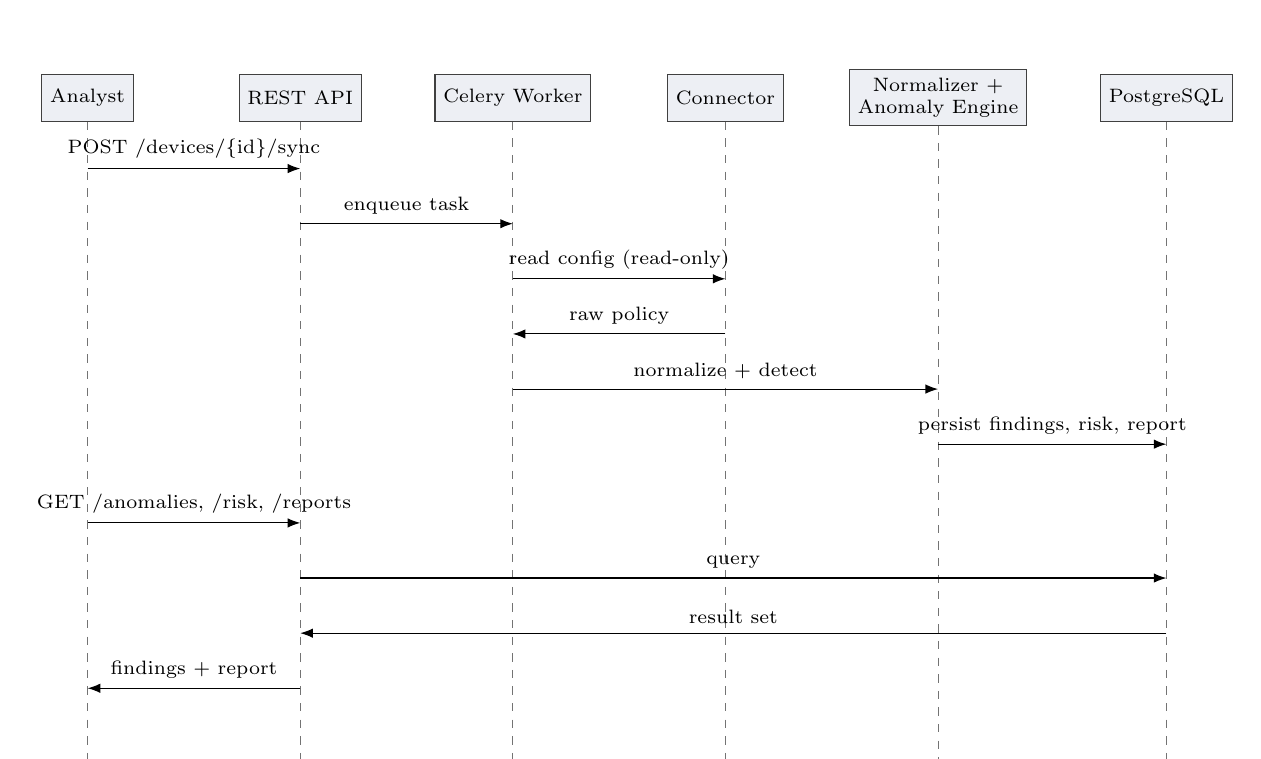
\begin{tikzpicture}[font=\scriptsize,
  act/.style={draw=black!75, fill=LightGray, minimum height=6mm, align=center, font=\scriptsize, inner sep=3pt},
  msg/.style={-{Latex[length=1.6mm]}}]
\node[act] (A)   at (0,0)    {Analyst};
\node[act] (API) at (2.7,0)  {REST API};
\node[act] (W)   at (5.4,0)  {Celery Worker};
\node[act] (C)   at (8.1,0)  {Connector};
\node[act] (N)   at (10.8,0) {Normalizer +\\Anomaly Engine};
\node[act] (DB)  at (13.7,0) {PostgreSQL};
\foreach \n in {A,API,W,C,N,DB} \draw[dashed, black!55] (\n.south) -- ++(0,-8.2);
\draw[msg] (0,-0.9)   -- node[above]{POST /devices/\{id\}/sync} (2.7,-0.9);
\draw[msg] (2.7,-1.6) -- node[above]{enqueue task} (5.4,-1.6);
\draw[msg] (5.4,-2.3) -- node[above]{read config (read-only)} (8.1,-2.3);
\draw[msg] (8.1,-3.0) -- node[above]{raw policy} (5.4,-3.0);
\draw[msg] (5.4,-3.7) -- node[above]{normalize + detect} (10.8,-3.7);
\draw[msg] (10.8,-4.4)-- node[above]{persist findings, risk, report} (13.7,-4.4);
\draw[msg] (0,-5.4)   -- node[above]{GET /anomalies, /risk, /reports} (2.7,-5.4);
\draw[msg] (2.7,-6.1) -- node[above]{query} (13.7,-6.1);
\draw[msg] (13.7,-6.8)-- node[above]{result set} (2.7,-6.8);
\draw[msg] (2.7,-7.5) -- node[above]{findings + report} (0,-7.5);
\end{tikzpicture}}
\caption{Sequence diagram: end-to-end policy acquisition, normalization, anomaly analysis, and reporting.}
\label{fig:seq-pipeline}
\end{figure}

The sequence begins synchronously. The analyst issues \texttt{POST}~\path{/api/v1/devices/{device_id}/poll}; the API verifies the device exists and that a credential is configured (returning \texttt{409} if absent), inserts an \texttt{AcquisitionJob} row with status \texttt{queued}, dispatches \texttt{poll\_device.delay(job\_id)} onto the \texttt{acquisition} queue, and immediately returns \texttt{202 Accepted} with the \texttt{job\_id} --- performing no firewall I/O in the request cycle.

The remainder runs asynchronously as an automatic chain. The \texttt{poll\_device} worker decrypts the credential in memory, resolves the vendor type, sets the job \texttt{running}, builds the connector, calls \texttt{collect()}, stores the raw artifacts with their SHA-256 manifest, updates the device's freshness and firmware, sets the job \texttt{success} or \texttt{partial\_success}, and on either success state chains \texttt{normalize\_device.delay(job\_id)} onto the \texttt{normalization} queue. The \texttt{normalize\_device} worker loads the job's artifacts from disk and runs \texttt{parse\_artifacts} $\rightarrow$ \texttt{normalize\_payloads} $\rightarrow$ \texttt{persist\_result} (the idempotent Schema~v4 upsert), then chains \texttt{run\_anomaly\_analysis\_task.delay(device\_id)} onto the \texttt{analysis} queue.

The \texttt{run\_anomaly\_analysis} worker opens an \texttt{AnomalyExecutionLog} (\texttt{status="running"}), reconstructs the \texttt{NormalizationResult} via \texttt{load\_normalized\_result}, calls \texttt{analyze(result)}, maps each \texttt{Finding} \texttt{(device\_id, rule\_uuid)} onto its \texttt{PolicyRule.rule\_id} (skipping rules absent from the repository rather than guessing), inserts the \texttt{RuleAnomaly} rows, finalises the log with \texttt{completed} and \texttt{findings\_count}, and as a best-effort final step calls \texttt{run\_risk(db, run\_id)} --- a risk failure must never fail the analysis. (For cross-device detectors an all-scope run is invoked with \texttt{device\_id=None}, analysing every device together.) Optionally, the analyst then triggers \texttt{POST}~\path{/api/v1/cti/run} (enrichment and correlation, with a follow-on risk recompute) and \texttt{POST}~\path{/api/v1/reports/generate} (the evidence-grounded report, persisted even on provider failure).

Throughout, the frontend never blocks: it polls job and run status through the read-only endpoints \texttt{GET /api/v1/jobs/\{job\_id\}}, \texttt{GET /api/v1/anomalies/runs} and the resource readers, then renders findings, risk, CTI and reports from PostgreSQL. The diagram thus makes visible the platform's governing rule --- slow, fallible, external work is confined to the worker tier behind the Redis broker, while the request cycle does only fast transactional work and read-back.

\chapter{Implementation and Testing}
\label{ch:implementation}

This chapter documents the realized LuminaFPM system: how the strictly read-only, multi-vendor firewall anomaly management platform described in the preceding chapters was actually built, and how the resulting engine was validated against ground truth. The chapter is presented in two parts. \emph{Part~A} (this half) covers \textbf{implementation} --- the development environment, the project layout, and a layer-by-layer account of the read-only data pipeline (acquisition $\rightarrow$ parsing $\rightarrow$ normalization $\rightarrow$ deterministic anomaly detection $\rightarrow$ risk scoring $\rightarrow$ threat intelligence $\rightarrow$ AI-assisted reporting), followed by the REST API surface and the React front-end console. \emph{Part~B} continues with \textbf{testing}: the benchmark acceptance gate, the unit/integration test suite, and the lab-based end-to-end validation. Throughout, the description is grounded in concrete file paths, class and function names, database tables, and REST endpoints from the delivered codebase rather than the original Term-1 proposal; where the build deliberately scopes below the full specification, this is stated plainly.

\section{Implementation Overview}
\label{sec:ch4-impl-overview}

LuminaFPM is implemented as a containerized, multi-service application orchestrated by Docker Compose. The backend is a Python/FastAPI application backed by a Celery worker pool, with PostgreSQL as the system of record and Redis as the Celery broker and result backend. The front end is a React/TypeScript single-page application served (in development) by Vite. Two backing data stores (PostgreSQL~16, Redis~7) and an optional Tor SOCKS proxy complete the runtime topology.

The implementation faithfully realizes the platform's single non-negotiable architectural principle: it is \textbf{strictly read-only against firewalls}. Every vendor connector issues only read verbs (\texttt{GET}, \texttt{show}, \texttt{monitor}, \texttt{keygen}); no module anywhere in the acquisition layer contains a write verb (\texttt{set}, \texttt{edit}, \texttt{delete}, \texttt{move}, or \texttt{commit}). All ``mutating'' HTTP calls the system makes are POSTs to its \emph{own} API that trigger internal analysis jobs (synchronize, analyze, enrich, generate, benchmark); none of them ever reaches a firewall to change its configuration.

A second, equally load-bearing principle governs the analysis engines: \textbf{detection is deterministic and reads the normalized model only}. The raw FortiGate JSON and Palo Alto XML are acquisition and parser inputs; they are never analyzed directly. The anomaly engine consumes exclusively the canonical normalized repository, the AI layer \emph{explains} findings but never \emph{detects} them, and every analysis engine cleanly separates a pure scoring/logic module (no database, no I/O) from a database-backed runner that persists results idempotently per analysis run. These two principles --- read-only acquisition and deterministic, normalized-model detection --- recur in every section below.

The v1 vendor scope is \textbf{Fortinet FortiGate (FortiOS REST/JSON) and Palo Alto Networks PAN-OS (XML API) only}. Cisco, which appeared in the Term-1 proposal, is de-scoped from v1 and is treated as future work; a small number of dormant Cisco/ASA code paths survive in the front end and are flagged as such.

\section{Development Environment and Tools}
\label{sec:ch4-devenv}

The system was developed against the technology stack summarized in Table~\ref{tab:ch4-stack}. The backend runs on Python~3.11 (base image \texttt{python:3.11-slim}); the front end runs on Node~22.

\begin{table}[!ht]
\centering
\caption{Core technology stack and tooling.}
\label{tab:ch4-stack}
\small
\begin{tabular}{L{3.0cm}L{4.0cm}L{6.4cm}}
\hline
\hcell{Concern} & \hcell{Choice} & \hcell{Role} \\
\hline
Web framework & FastAPI + Uvicorn & ASGI REST API surface (routers, dependency injection, OpenAPI). \\
ORM / DB & SQLAlchemy + PostgreSQL~16 & Models and session management; canonical system of record. \\
Migrations & Alembic & Versioned schema migrations (Schema~v4). \\
Validation & Pydantic + pydantic-settings & Request/response schemas; typed environment configuration. \\
Task queue & Celery (Redis broker) & Asynchronous acquisition / normalization / analysis / CTI / reporting jobs. \\
Cache / broker & Redis~7 & Celery broker and result backend; SSE pub/sub. \\
Crypto & cryptography (Fernet) & Symmetric encryption of stored device credentials. \\
XML hardening & defusedxml & Hardened PAN-OS XML parsing (entity-expansion safe). \\
HTTP client & requests & FortiGate REST and CTI API calls. \\
Front-end build & Vite + @vitejs/plugin-react & Dev server, build, lint, typecheck. \\
UI framework & React~19 + TypeScript~5.7 & Single-page console; incremental TS migration. \\
LLM provider & Google Gemini (+ offline fallback) & Evidence-grounded SOC reporting; deterministic offline renderer. \\
Orchestration & Docker Compose & Multi-service runtime (db, redis, api, celery\_worker, celery\_beat, frontend). \\
\hline
\end{tabular}
\end{table}

Two reproducibility caveats are documented honestly rather than smoothed over. First, the backend \texttt{requirements.txt} is \textbf{unpinned} --- every package is named but no version is fixed --- so builds are not deterministic across time; the only version constraint is the Python base image. Front-end dependencies, by contrast, are pinned with caret (\textasciicircum{}) ranges in \texttt{package.json}. Second, the front-end Docker image runs the \emph{Vite development server} (not a production build): an Nginx production-serve configuration (\texttt{frontend/nginx.conf}) exists but is not wired into the Compose deployment.

The Compose stack defines six active services. The \texttt{api} service runs Uvicorn with \texttt{-{}-reload}; the \texttt{celery\_worker} runs under \texttt{watchmedo auto-restart} and explicitly consumes the queues \texttt{acquisition,\,normalization,\,analysis,\,cti,\,reporting,\,celery} (without the explicit \texttt{-Q} list the routed tasks would never run); and the \texttt{celery\_beat} service drives the scheduler tick every 60 seconds that powers the Settings scheduling feature. PostgreSQL and Redis are \emph{not} published to the host (internal Docker network only), a deliberate security posture. A \texttt{tor-proxy} service and a commented-out ``Robin'' dark-web OSINT pair (\texttt{robin\_ui}/\texttt{robin\_api}) support the optional, off-by-default threat-intelligence subsystem and are not part of the running v1 stack.

\section{Project Structure}
\label{sec:ch4-structure}

The repository is split into a Python backend, a React/TypeScript front end, and a self-contained lab provisioner used only for testing. The principal directories are shown in Listing~\ref{lst:ch4-tree}.

\begin{lstlisting}[caption={LuminaFPM repository structure (abridged).},label={lst:ch4-tree}]
lumina-fpm/
  backend/
    main.py                  # FastAPI app; mounts LTI router + 14 core routers
    core/
      config.py              # Settings (pydantic-settings); env reference
      security.py            # Fernet credential encryption
      logging.py             # structured, secret-safe logging
    api/routes/              # REST routers (vendors, devices, rules, anomalies,
                             #   risk, cti, reports, benchmark, jobs, ...)
    services/
      acquisition/           # read-only connectors (base, fortigate, paloalto,
                             #   registry, storage, models, errors)
      parsing/               # vendor parsers (fortigate JSON, paloalto XML)
      normalization/         # canonical, model, engine, persist, loader
      anomaly/               # engine.py, detectors.py, model.py
      risk/                  # scorer.py (pure), runner.py (DB)
      cti/                   # extract.py, providers.py, runner.py
      llm/                   # providers.py, prompts.py, reporter.py
      benchmark/             # scorer.py, ground_truth.py, runner.py
      lumina_threat_intel/   # optional, off-by-default LTI subsystem
    tasks/                   # Celery tasks (acquisition, normalization, analysis)
    alembic/                 # schema migrations (Schema v4)
    tests/                   # unit + integration tests
  frontend/
    src/
      app.jsx                # hash router + app-level state
      api.js                 # legacy aggregate loader -> LFPMContext
      lib/api.ts             # typed client (new single source of truth)
      context/LFPMContext.jsx
      dashboard.jsx audit.jsx inspector.jsx topology.jsx threats.jsx
      risk.tsx reports.tsx cti.tsx benchmark.tsx   # newer typed screens
  lab/
    benchmark_dataset.py     # ground-truth anomaly matrix (source)
    benchmark_ground_truth.json
    provision_benchmark.py   # WRITE tooling (separate keys; NOT the platform)
  docker-compose.yml
\end{lstlisting}

A structural note: \texttt{lab/} contains \emph{write} tooling that provisions known-bad policies onto the lab firewalls for benchmarking. It uses separate credentials and is explicitly \textbf{not} part of the LuminaFPM platform --- the platform itself never writes. Because the \texttt{lab/} directory is not mounted into the API container, the authoritative ground-truth matrix is mirrored inside the backend at \texttt{services/benchmark/ground\_truth.py}.

\section{Acquisition Layer}
\label{sec:ch4-acquisition}

The acquisition layer (\texttt{backend/services/acquisition/}) performs read-only extraction of firewall configuration from FortiGate (FortiOS REST/JSON) and Palo Alto (PAN-OS XML API). Connectors collect data only --- no anomaly logic, no write or commit --- and run asynchronously inside Celery workers, never inside the FastAPI request cycle.

\subsection*{Connector contract}

\texttt{base.py} defines the read-only connector contract. \texttt{ConnectorInterface} (an \texttt{abc.ABC}) declares three abstract methods: \texttt{authenticate()} (establish/validate auth, no config changes), \texttt{validate\_connection()} (a lightweight read confirming connectivity and auth), and \texttt{collect()} (full read-only extraction returning an \texttt{AcquisitionBundle}). The accompanying \texttt{ConnectorConfig} dataclass carries the connection parameters resolved from the device record and the \emph{decrypted} credential, which is held in memory only and never persisted. Its fields include \texttt{device\_id}, \texttt{vendor\_type} (\texttt{fortinet} or \texttt{paloalto}), \texttt{management\_ip}, the in-memory \texttt{secret}, \texttt{auth\_type}, \texttt{verify\_tls} (default \texttt{True}), \texttt{timeout\_seconds} (default 60), and --- critically --- \texttt{scheme} (default \texttt{"https"}), the HTTP-scheme override discussed below.

The \texttt{collect()} contract distinguishes \emph{required} from \emph{optional} endpoints: failure of an optional endpoint produces a warning and downgrades the bundle to \texttt{partial\_success}, whereas failure of a required endpoint (the policies) raises an \texttt{AcquisitionError}. The error taxonomy (\texttt{errors.py}) maps every failure mode to a normalized \texttt{code} and a \texttt{retryable} flag that drives the retry policy --- for example \texttt{AuthenticationError} (\texttt{AUTH\_FAILED}, non-retryable, to avoid lockout hammering), \texttt{ConnectionFailedError} (\texttt{CONNECTION\_FAILED}, retryable), and \texttt{TLSError} (\texttt{TLS\_FAILED}, non-retryable). Error messages are required to be secret-safe.

\subsection*{FortiGate connector}

\texttt{fortigate.py} implements \texttt{FortiGateConnector} (\texttt{vendor\_type="fortinet"}). Authentication uses a Bearer API token (a dedicated read-only API admin account) injected via \texttt{\_headers()}; \texttt{validate\_connection()} performs a cheap \texttt{GET} of \path{/api/v2/monitor/system/status}. There is exactly one HTTP helper, \texttt{\_get(path)} --- and \emph{no} write verb anywhere in the module, which is precisely how read-only is enforced at the code level. Its exception-to-error mapping converts \texttt{requests} SSL/timeout/connection exceptions and HTTP status codes (401$\rightarrow$\texttt{AuthenticationError}, 403$\rightarrow$\texttt{AuthorizationError}, 404$\rightarrow$\texttt{UnsupportedEndpointError}, other $\geq$400$\rightarrow$\texttt{ConnectionFailedError}) into the normalized taxonomy. The connector iterates a static endpoint table covering policies, address objects, address groups, service objects, service groups, and device metadata (all required), plus interfaces and schedules (optional). Each successful response is captured as a \texttt{RawArtifact}.

\subsection*{Palo Alto connector}

\texttt{paloalto.py} implements \texttt{PaloAltoConnector} (\texttt{vendor\_type="paloalto"}) against the PAN-OS XML API. Authentication uses an \texttt{X-PAN-KEY} header; when \texttt{auth\_type=="panos\_userpass"} the connector issues a read-only \texttt{type=keygen} request and regex-extracts an ephemeral key. Because PAN-OS returns HTTP~200 with \texttt{status="error"} in the XML body for bad credentials, the connector additionally inspects the body for \texttt{status="error"} plus an ``Invalid credential'' marker. Configuration is read with \texttt{type=config\&action=show} over the unqualified vsys xpath \texttt{/config/devices/entry/vsys/entry/<leaf>}, which is the form proven to work against the single-vsys lab device. Required leaves map to policies, address objects/groups, and service objects/groups; the \texttt{zone} leaf is recommended and degrades to a warning on failure. PAN-OS NAT is a separate policy type and is deferred to future work.

\subsection*{The HTTP-scheme override (lab escape hatch)}

A documented deviation handles a real lab quirk: the lab FortiGate's \texttt{httpsd} will not bind port~443, so its management API is reachable only over plain HTTP. The escape hatch is implemented end-to-end. \texttt{core/config.py} exposes \texttt{FIREWALL\_INSECURE\_HTTP\_HOSTS} (a CSV list property), documented as \textbf{lab-only --- never to be set in production}, since API tokens would otherwise traverse unencrypted. Both call sites that build a \texttt{ConnectorConfig} --- the acquisition task and the device connectivity-test route --- select the scheme per host: \texttt{scheme = "http" if device.management\_ip in settings.firewall\_insecure\_http\_hosts else "https"}. Crucially, only \texttt{FortiGateConnector.\_base\_url()} honors \texttt{scheme}; \texttt{PaloAltoConnector.\_base\_url()} hardcodes \texttt{https://} and ignores it, so the override is FortiGate-specific.

\subsection*{Raw persistence}

\texttt{storage.py} persists each raw response to disk (under \texttt{\{vendor\}/\{device\_id\}/\{job\_id\}/}) so the parser can replay without re-polling, and writes an \texttt{acquisition\_manifest.json} carrying per-artifact SHA-256 hashes. This gives the pipeline auditability and replayability: every analysis can be traced back to a specific, hashed raw capture.

\section{Parsing and Normalization}
\label{sec:ch4-parse-norm}

\subsection*{Parsing}

The parsing layer (\texttt{backend/services/parsing/}) converts raw vendor responses into structured, \emph{vendor-tagged} dataclasses without any canonicalization or anomaly logic --- raw vendor values are deliberately preserved at this stage (e.g.\ FortiGate \texttt{accept} versus PAN \texttt{allow}). Both parsers emit a uniformly shaped \texttt{ParsedDevicePayload} containing \texttt{ParsedRule}, \texttt{ParsedAddressObject}, \texttt{ParsedAddressGroup}, \texttt{ParsedServiceObject}, and \texttt{ParsedServiceGroup} lists, so the downstream normalizer can consume either vendor uniformly. The FortiGate JSON parser (validated against a real FortiOS~7.0.5 response) maps FortiGate subnet/mask notations to CIDR and builds a structured \texttt{security\_profiles} dictionary; the PAN-OS XML parser uses \texttt{defusedxml} when available and derives logging from \texttt{log-start}/\texttt{log-end}.

\subsection*{Normalization and the canonical model}

The normalization layer (\texttt{backend/services/normalization/}) converts vendor-tagged parser models into the canonical normalized policy model and the object/service correlation model. It is \textbf{deterministic and idempotent}: the same input always yields the same output, and re-running a sync never duplicates rows. \texttt{canonical.py} holds pure mapping functions (no database, no I/O): \texttt{canonical\_action} collapses vendor actions into a small enum (\texttt{accept}/\texttt{allow}$\rightarrow$\texttt{allow}, \texttt{deny}, \texttt{drop}, \texttt{reset}, \texttt{ipsec}); \texttt{canonical\_logging} and \texttt{canonical\_inspection} reduce heterogeneous logging/inspection settings to \texttt{true}/\texttt{false}/\texttt{unknown}, with the inspection result driving the unprotected-allow detector.

Two pieces of ANY-handling logic are central to correctness. For \emph{objects}, \texttt{is\_any\_object} recognizes the names \{\texttt{all},\,\texttt{any}\} and the values \{\texttt{0.0.0.0/0},\,\texttt{::/0},\,\dots\} and canonicalizes them to the single ANY sentinel \texttt{("any",\,"0.0.0.0/0")}. For \emph{services}, \texttt{canonical\_service} expands FortiGate's broad predefined services via a \texttt{\_BROAD\_SERVICES} map (\texttt{all}$\rightarrow$\texttt{(any,None,None)}, \texttt{all\_tcp}$\rightarrow$\texttt{(tcp,1,65535)}, etc.), while PAN-OS predefined names (\texttt{service-https}, \texttt{any}, \dots) resolve through a \texttt{PREDEFINED\_SERVICES} table. Without this expansion FortiGate's \texttt{ALL} service would key as \texttt{unknown:any} and the coverage/shadowing/redundancy logic would fail to treat it as the ANY sentinel. The \texttt{service\_key()} helper produces stable keys (\texttt{app:<id>}, \texttt{<proto>:any}, or \texttt{<proto>:<ps>-<pe>}) that the detection engine compares as sets.

The deterministic correlation engine (\texttt{engine.py::normalize\_payloads}) implements \textbf{correlation, not merge}: vendor objects and services remain separate rows for ownership and traceability, while canonical \texttt{normalized\_object} / \texttt{normalized\_service} records sit above them, linked by mapping records. Matching is confidence-scored: an exact name-and-value match scores 1.00 (\texttt{exact\_name\_value}); a same-value, different-name match scores 0.90 (\texttt{exact\_value}) and raises a naming-inconsistency candidate. Each rule is normalized into a \texttt{NormalizedRule} carrying canonical action, logging/inspection flags, correlation-key lists (\texttt{src\_object\_keys}, \texttt{dst\_object\_keys}, \texttt{service\_keys}), and a \texttt{normalized\_content\_hash}. \texttt{persist.py} writes the result idempotently into Schema~v4 using documented natural keys (e.g.\ \texttt{PolicyRule} upserts on \texttt{(device\_id,\,vdom\_vsys,\,vendor\_uuid)}), and \texttt{loader.py} reconstructs a byte-identical \texttt{NormalizationResult} from persisted rows so the anomaly engine can analyze the normalized repository across a persist$\rightarrow$load round-trip --- a contract that is essential for the cross-device detectors, which load all devices at once. The richer group cycle-detection and the 0.30/0.40/0.20 confidence tiers from the specification are documented-but-not-implemented at this snapshot.

\section{Anomaly Detection Engine}
\label{sec:ch4-anomaly}

The anomaly detection engine is the analytical heart of LuminaFPM. It is implemented in \texttt{backend/services/anomaly/} (\texttt{engine.py}, \texttt{detectors.py}, \texttt{model.py}) and embodies the platform's core thesis: that firewall misconfigurations can be detected \emph{deterministically and explainably} by reasoning over a unified, cross-vendor normalized model. This section first develops the formal set-theoretic model that gives the engine its conceptual rigor, then describes the deterministic implementation, the severity/confidence and detection-mode machinery, the cross-device detectors, and finally the implemented taxonomy.

\subsection{The Set-Theoretic Conceptual Model}
\label{sec:ch4-settheory}

Conceptually, each normalized firewall rule $r$ is modeled as a tuple of sets over a small number of dimensions:
\[
r = \langle\, S_r,\; D_r,\; V_r,\; a_r \,\rangle
\]
where $S_r$ is the set of canonical source-object keys, $D_r$ the set of destination-object keys, $V_r$ the set of canonical service keys, and $a_r \in \{\texttt{allow},\texttt{deny},\texttt{drop},\texttt{reset},\texttt{ipsec},\dots\}$ the canonical action. The \emph{match space} of a rule is the Cartesian product $M_r = S_r \times D_r \times V_r$ --- the set of traffic flows the rule applies to. A distinguished \emph{ANY} sentinel ($\top$) is treated as the universal set on its dimension; an empty set on a dimension is likewise interpreted as ANY. Two rules are then compared by elementary set relations on their three dimensions, and the anomaly classes follow directly:

\begin{itemize}[leftmargin=1.4em]
  \item \textbf{Shadowing} ($r_i$ shadows $r_j$, $i<j$): an earlier \emph{blocking} rule whose match space covers the later rule, $M_{r_j} \subseteq M_{r_i}$, so the later rule can never match --- $r_i$ is a superset of $r_j$ on all three dimensions.
  \item \textbf{Redundancy}: a later rule with the same action whose match space is covered by an earlier rule ($M_{r_j} \subseteq M_{r_i}$, $a_i = a_j$) but is \emph{not} an exact duplicate --- the later rule adds nothing.
  \item \textbf{Duplicate}: set equivalence with identical action --- $S_i{=}S_j \wedge D_i{=}D_j \wedge V_i{=}V_j \wedge a_i{=}a_j$.
  \item \textbf{Conflict}: overlapping match spaces with \emph{differing} actions --- $M_{r_i} \cap M_{r_j} \neq \varnothing \wedge a_i \neq a_j$ --- the rulebase expresses two contradictory decisions for the same flows.
  \item \textbf{Generalization} is the dual of shadowing (a later, broader rule supersets an earlier, narrower one of the same action); in v1 the engine surfaces this family through the redundancy/shadowing pair rather than as a distinct emitted type.
\end{itemize}

Single-rule anomalies are expressed just as naturally: an \emph{overly permissive} rule is $S_r = D_r = V_r = \top$ with $a_r = \texttt{allow}$ (any/any/any); an \emph{any-to-sensitive} rule has $S_r = \top$ and $D_r$ intersecting the sensitive-asset class; a \emph{wide port range} is a single service spanning more than 1024 ports. This set-theory framing is the \emph{formal} conceptual model; the \emph{implementation} (below) is a deterministic rule-based engine over the normalized model --- it is not machine learning, and it uses no statistics, randomness, or training data.

\subsection{The Deterministic Engine}
\label{sec:ch4-det-engine}

The engine entry point is \texttt{engine.py::analyze(result: NormalizationResult) -> List[Finding]}. It iterates a fixed-order tuple, \texttt{detectors.ALL\_DETECTORS}, and concatenates each detector's findings. It reads the normalized model \emph{only} --- no database, no network, no LLM. Determinism is guaranteed by three mechanisms: (a)~a fixed detector order; (b)~a stable rule sort, \texttt{\_sorted\_rules()}, keyed on \texttt{(device\_id, rule\_order, vendor\_uuid, rule\_name)}; and (c)~the use of \texttt{itertools.combinations} over the sorted list for pairwise detectors, so the ``earlier'' rule in any pair always has the lower \texttt{rule\_order}. No randomness, wall-clock, or nondeterministic dictionary iteration is used. (The earlier mock predecessor, \texttt{anomaly\_engine.py}, which generated random anomalies on random rules, is explicitly flagged as a specification violation and fully superseded by this package.)

The set logic operates directly on the canonical correlation keys. Module-level constants define the ANY sentinels (\texttt{ANY\_OBJECT\_KEY}, \texttt{ANY\_SERVICE\_KEY}), the action classes (\texttt{\_BLOCKING\_ACTIONS = \{deny, drop, reset\}}, \texttt{\_ALLOW\_ACTIONS = \{allow, ipsec\}}), the wide-port threshold (1024), the object-sprawl threshold (50), and the sensitive classes (\texttt{\{admin, database, critical\}}). Set helpers implement the relations from Section~\ref{sec:ch4-settheory}: \texttt{\_covers(a,b)} returns true when $a$ is ANY/empty or $b \subseteq a$; \texttt{\_sets\_overlap(a,b)} returns true when either side is ANY/empty or the sets intersect; and \texttt{\_same\_access(a,b)} requires equality on source, destination, and service. The end-to-end flow --- from normalized rules through the per-detector set comparisons to persisted \texttt{Finding}s --- is shown in Figure~\ref{fig:anomflow}.

\begin{figure}[htbp]
\centering
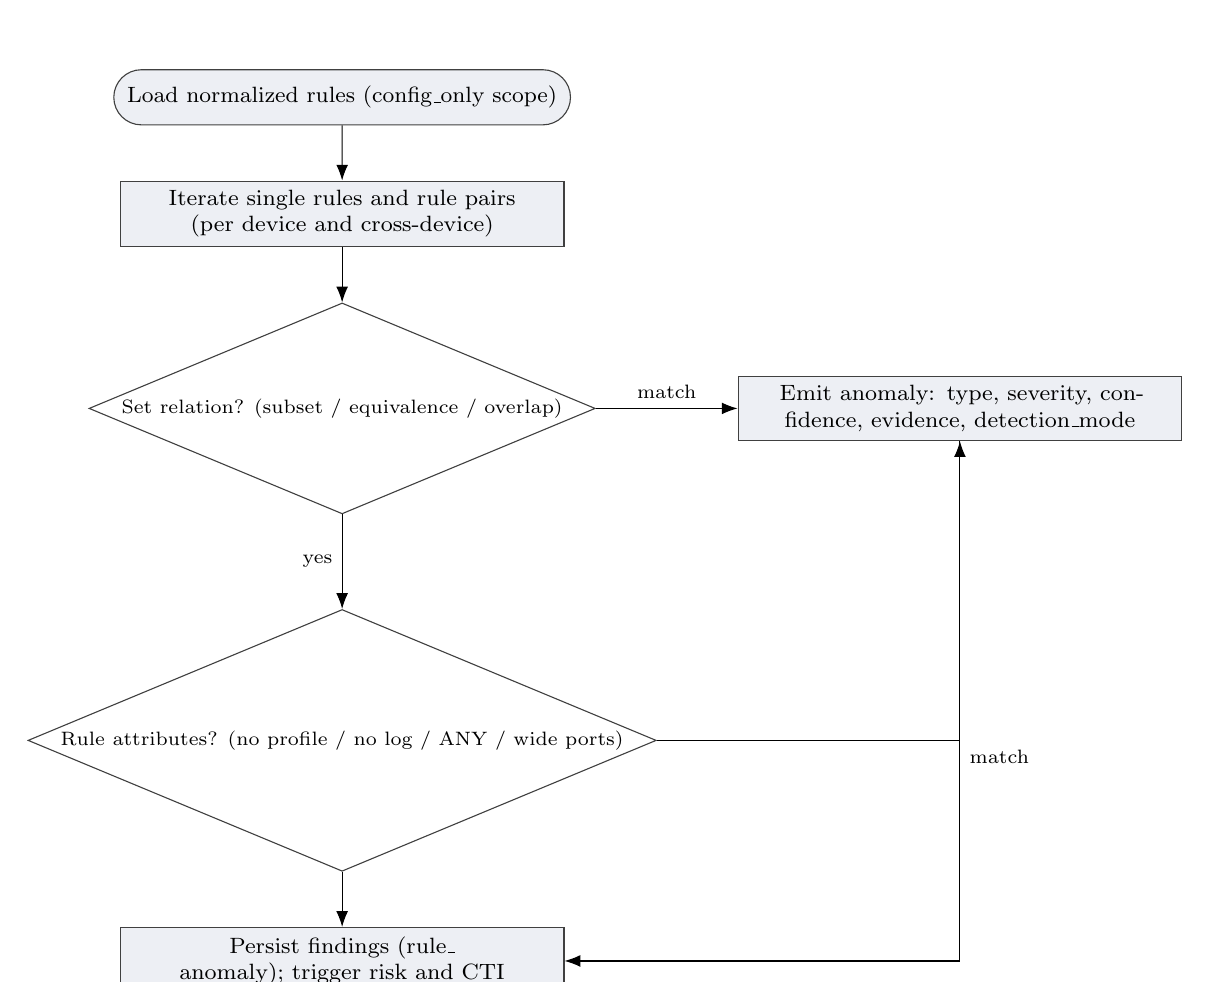
\begin{tikzpicture}[
  node distance=7mm,
  term/.style={draw=black!75, rounded rectangle, fill=LightGray, font=\footnotesize, align=center, minimum height=7mm, inner sep=4pt},
  box/.style={draw=black!75, fill=LightGray, text width=5.4cm, align=center, font=\footnotesize, minimum height=8mm},
  dec/.style={draw=black!75, diamond, aspect=2.4, fill=white, align=center, font=\scriptsize, inner sep=1pt},
  flow/.style={-{Latex[length=2mm]}}]
\node[term] (st) {Load normalized rules (config\_only scope)};
\node[box, below=of st] (pair) {Iterate single rules and rule pairs (per device and cross-device)};
\node[dec, below=of pair] (d1) {Set relation? (subset / equivalence / overlap)};
\node[dec, below=12mm of d1] (d2) {Rule attributes? (no profile / no log / ANY / wide ports)};
\node[box, right=18mm of d1] (emit) {Emit anomaly: type, severity, confidence, evidence, detection\_mode};
\node[box, below=of d2] (persist) {Persist findings (rule\_anomaly); trigger risk and CTI};
\draw[flow] (st) -- (pair);
\draw[flow] (pair) -- (d1);
\draw[flow] (d1) -- node[left,font=\scriptsize]{yes} (d2);
\draw[flow] (d1) -- node[above,font=\scriptsize]{match} (emit);
\draw[flow] (d2) -| node[below right,font=\scriptsize]{match} (emit);
\draw[flow] (d2) -- (persist);
\draw[flow] (emit) |- (persist);
\end{tikzpicture}
\caption{Control flow of the deterministic anomaly-detection engine.}
\label{fig:anomflow}
\end{figure}

Each detector emits zero or more \texttt{Finding} objects. \texttt{Finding} is a pure, database-independent dataclass; the anomaly Celery task later maps each one onto a \texttt{RuleAnomaly} row by resolving \texttt{(device\_id, rule\_uuid) -> PolicyRule.rule\_id}. Its fields are \texttt{anomaly\_type}, \texttt{device\_id}, \texttt{rule\_uuid}, \texttt{severity}, \texttt{confidence}, \texttt{description}, \texttt{recommendation}, \texttt{evidence}, the optional cross-device peers \texttt{related\_device\_id}/\texttt{related\_rule\_uuid}, and \texttt{detection\_mode}. Crucially, \textbf{every finding is explainable}: the \texttt{evidence} dictionary carries the concrete facts that produced it (device, vendor, rule name and order, vendor UUID, action), which is what makes the AI reporting layer able to \emph{explain without re-detecting}.

\subsection{Severity, Confidence, and Detection Mode}
\label{sec:ch4-sev-mode}

Severity and confidence are assigned per anomaly \emph{type}, not learned: each detector hard-codes a severity in \{\texttt{critical}, \texttt{high}, \texttt{medium}, \texttt{low}\} and a confidence in $[0,1]$, reflecting how strongly the configuration evidence implies the finding (see Table~\ref{tab:ch4-anomaly-taxonomy}). Because severity is fixed per type and independent of the engine's matching, it can itself be validated by the benchmark (Part~B).

The \texttt{detection\_mode} field records \emph{what kind of evidence} a finding rests on. The specification defines four/five modes: \texttt{config\_only} (derivable from configuration alone --- the v1 core), \texttt{conditional} (needs logs, hit-counts, or history), \texttt{simulated}/\texttt{benchmark\_simulated} (derived from lab metadata and required to be labeled as such), and \texttt{future\_enhanced} (needs enterprise telemetry); the CTI runner adds a runtime fifth mode, \texttt{cti}. In the delivered code, \textbf{all fourteen detectors emit \texttt{config\_only}} (the \texttt{Finding} default), and the only non-\texttt{config\_only} finding produced is \texttt{threat\_exposure} (\texttt{detection\_mode="cti"}), written by the CTI runner. The \texttt{conditional}, \texttt{simulated}, and \texttt{future\_enhanced} modes are defined in the schema but not yet emitted by any detector --- a deliberate v1 scope limit, not an omission.

\subsection{Cross-Device Detectors}
\label{sec:ch4-crossdev}

Two detectors operate \emph{across} devices and surface the platform's core cross-vendor innovation as concrete findings. \texttt{\_cross\_device\_pairs()} yields all sorted-rule combinations whose \texttt{device\_id} differs, and equivalence is always established through normalized correlation keys, never raw vendor names.

\texttt{detect\_cross\_device\_inconsistency} fires when two rules on different devices have \emph{equal} canonical source/destination/service sets (\texttt{\_same\_access}) but \emph{different} actions --- for example, a FortiGate that \texttt{allows} exactly the canonical access a Palo Alto \texttt{denies}. This is rated \texttt{critical} (confidence 0.85): a conflicting access decision across the fleet is precisely the class of error that single-vendor tools cannot see. \texttt{detect\_cross\_device\_security\_posture\_inconsistency} fires when two cross-device rules have equal sets and \emph{both} allow, but differ in \texttt{logging\_enabled} or \texttt{security\_inspection\_enabled} (e.g.\ one inspected, the other unprotected); it is rated \texttt{medium} (confidence 0.8). These two detectors are only meaningful because every device's rules are normalized into one shared key space --- the very capability the project set out to build.

\subsection{Anomaly Types and Policy-Rule Implementation}
\label{sec:ch4-anomaly-taxonomy}

The full specification defines a 46-type anomaly taxonomy. Version~1 ships the ``config-only core'': fourteen deterministic detectors (in \texttt{ALL\_DETECTORS}) emitting fourteen distinct \texttt{anomaly\_type} values, plus \texttt{threat\_exposure} written by the CTI runner, for fifteen persisted types in total. Table~\ref{tab:ch4-anomaly-taxonomy} lists every implemented type --- its description, the detection mode it is emitted in, and whether it is realized as a live policy-rule detector. Types from the broader framework that remain \emph{simulated} or \emph{future} (e.g.\ ordering anomaly, temporary-rule, poor-naming, zone-mismatch, NAT-risk, asymmetric-rule, and all \texttt{conditional}/\texttt{future\_enhanced} entries) are specified but \textbf{not implemented} in v1 and are marked accordingly.

{\footnotesize
\begin{longtable}{L{3.3cm}L{5.6cm}C{1.4cm}C{1.7cm}C{1.4cm}}
\caption{Implemented anomaly taxonomy: the config-detectable core actually emitted by the engine, versus the simulated/future remainder of the 46-type framework.}
\label{tab:ch4-anomaly-taxonomy}\\
\hline
\hcell{Anomaly type} & \hcell{Description} & \hcell{Severity} & \hcell{Detection mode} & \hcell{Policy-rule?} \\
\hline
\endfirsthead
\hline
\hcell{Anomaly type} & \hcell{Description} & \hcell{Severity} & \hcell{Detection mode} & \hcell{Policy-rule?} \\
\hline
\endhead
\hline
\endfoot
\hline
\endlastfoot
\texttt{unprotected\_\allowbreak allow} & Enabled allow rule with no security inspection enabled. & high & config\_only & Yes \\
\texttt{shadowing} & Earlier blocking rule whose set covers a later rule; later never matches. & high & config\_only & Yes \\
\texttt{redundancy} & Later rule (same action) fully covered by an earlier rule; adds nothing. & medium & config\_only & Yes \\
\texttt{duplicate\_\allowbreak rules} & Two rules with identical src/dst/service sets and identical action. & medium & config\_only & Yes \\
\texttt{conflict} & Overlapping match space with differing actions on the same device. & high & config\_only & Yes \\
\texttt{any\_to\_\allowbreak sensitive} & Allow from ANY source to a sensitive (admin/database/critical) asset. & critical & config\_only & Yes \\
\texttt{overly\_\allowbreak permissive} & Allow with ANY source, ANY destination, and ANY service. & critical & config\_only & Yes \\
\texttt{wide\_port\_\allowbreak range} & Allow referencing a service spanning more than 1024 ports. & medium & config\_only & Yes \\
\texttt{missing\_\allowbreak description} & Rule with empty/whitespace description (fires even when disabled). & low & config\_only & Yes \\
\texttt{missing\_\allowbreak logging} & Enabled rule with logging disabled. & medium & config\_only & Yes \\
\texttt{disabled\_\allowbreak rule\_\allowbreak review} & Disabled rule flagged for lifecycle review. & low & config\_only & Yes \\
\texttt{object\_\allowbreak sprawl} & More than 50 distinct objects on one side of a rule. & low & config\_only & Yes \\
\texttt{cross\_device\_\allowbreak inconsistency} & Equal canonical access but conflicting action across two devices. & critical & config\_only & Yes \\
\texttt{cross\_device\_\allowbreak security\_\allowbreak posture\_\allowbreak inconsistency} & Equal allow access but differing logging/inspection across devices. & medium & config\_only & Yes \\
\texttt{threat\_\allowbreak exposure} & Allow rule referencing an indicator a CTI provider flags malicious. & from CTI & cti & Yes (CTI runner) \\
Ordering, temporary-rule, poor-naming, zone-mismatch, NAT-risk, asymmetric-rule, $\dots$ & Remaining entries of the 46-type framework requiring logs, history, or telemetry. & varies & conditional / future\_\allowbreak enhanced & No (future) \\
\end{longtable}
}

The single-rule detectors map almost verbatim onto the set model: \texttt{unprotected\_allow} fires on an enabled allow rule with \texttt{security\_inspection\_enabled=="false"}; \texttt{overly\_permissive} on any/any/any allow; \texttt{any\_to\_sensitive} on an ANY-source allow whose destination keys include a sensitive-class object; \texttt{wide\_port\_range} when a service's \texttt{(port\_end - port\_start) > 1024}; and \texttt{object\_sprawl} when any side exceeds 50 distinct keys. The pairwise detectors implement the subset/equivalence/overlap relations of Section~\ref{sec:ch4-settheory} exactly, with each finding attributed to the appropriate rule and its peer recorded in \texttt{related\_rule\_uuid}.

\section{Risk Scoring}
\label{sec:ch4-risk}

Risk scoring (\texttt{backend/services/risk/}) converts deterministic findings into a normalized 0--100 composite score per rule and per device. The pure scorer (\texttt{scorer.py}) is database-free; the runner (\texttt{runner.py}) persists \texttt{RiskAssessment} rows idempotently per analysis run. (For traceability the persisted \texttt{calculation\_version} is the literal \texttt{"1.0.0"}; the comments reference Volume~8, so the model is referred to informally as the ``V8'' composite.)

The per-rule composite is the clamped sum of eight factors:
\[
\begin{aligned}
\text{risk} = \min\big(100,\ &\text{anomaly} + \text{exposure} + \text{asset\_sensitivity} + \text{security\_posture} \\
&{}+ \text{logging} + \text{cross\_vendor} + \text{cti} + \text{lifecycle}\big).
\end{aligned}
\]
\texttt{score\_rule(findings)} builds a \texttt{factors} dictionary in which only non-zero factors appear, and each factor is taken as a \emph{maximum} across findings so it stays inside its allotted range regardless of how many findings hit it. The severity-point constants are \texttt{critical}=35, \texttt{high}=22, \texttt{medium}=12, \texttt{low}=4. The \emph{anomaly} factor is the dominant severity plus a small ``stacked-findings'' compound bonus, $\max(\text{sev\_points}) + \min(8,\, 2(|\text{findings}|-1))$. A factor-contribution map routes specific anomaly types to specific factors --- for example \texttt{overly\_permissive}$\rightarrow$exposure ($+20$), \texttt{any\_to\_sensitive}$\rightarrow$asset\_sensitivity ($+15$), \texttt{unprotected\_allow}$\rightarrow$security\_posture ($+20$), \texttt{missing\_logging}$\rightarrow$logging ($+15$), and the two cross-device types$\rightarrow$cross\_vendor ($+28$/$+18$). The \emph{cti} factor is added only when a \texttt{threat\_exposure} finding is present, scaled by the provider's verdict severity (critical=38, high=28, medium=18, low=10). In v1 the \emph{lifecycle} factor is fed only by \texttt{disabled\_rule\_review}; no age/history/drift factors exist yet.

Scores are bucketed by \texttt{tier\_of(score)} into \texttt{critical} ($\geq$90), \texttt{high} ($\geq$70), \texttt{medium} ($\geq$40), \texttt{low} ($\geq$1), and \texttt{informational} (0). The device-level blend (\texttt{score\_device}) deliberately weights the worst rule rather than averaging: it takes the top-5 rule scores and computes $0.6\,\text{max} + 0.4\,\text{avg(top5)}$, then adds a modifier $\min(10,\, 4\times\text{critical\_count})$ before clamping to 100, so a single critical rule is not diluted by many benign ones. Separately from the eight rule-level factors, the device score also admits an optional device-scope \texttt{firmware\_modifier} (\texttt{critical}=40, \texttt{high}=30, \texttt{medium}=18, \texttt{low}=10 points, with the result still clamped to 100) fed by the firmware-CVE intelligence axis (\S\ref{sec:ch4-cti}); this is a device-level adjustment, \emph{not} a ninth rule-level factor. The runner scores every active \texttt{PolicyRule}, is idempotent per run (it deletes that run's prior assessments but preserves other runs as history), and is read-only against firewalls.

\section{Threat Intelligence (CTI)}
\label{sec:ch4-cti}

The CTI layer (\texttt{backend/services/cti/}) enriches the normalized network objects with API-based threat intelligence and correlates malicious indicators back to the rules that expose them. It is API-based and strictly read-only against firewalls.

\textbf{Data minimization} is enforced before any network call (\texttt{extract.py}). \texttt{extract\_indicators} dedupes objects by value and applies the rule \texttt{if not is\_public and not allow\_internal: continue} --- so RFC1918/loopback/link-local/reserved addresses are \emph{never} sent to external providers unless an operator explicitly opts in. The ANY sentinels (\texttt{0.0.0.0/0}, \texttt{::/0}) are guarded out entirely and never become indicators, and single-host \texttt{/32} (and \texttt{/128}) CIDRs are canonicalized to bare IPs. Indicator types are limited to \{\texttt{ip\_address}, \texttt{cidr}, \texttt{fqdn}\}.

Providers (\texttt{providers.py}) implement a common \texttt{CtiProvider} ABC returning a \texttt{CtiVerdict}. \texttt{LabOfflineProvider} is always present and \emph{network-free}: it carries a small \texttt{KNOWN\_BAD} dictionary (e.g.\ a long-standing Tor-exit/abuse IP) so CTI is demonstrable offline and deterministically. \texttt{AbuseIPDBProvider} performs real REST lookups against AbuseIPDB but is activated only when an API key is configured, and it returns \texttt{None} (never an exception) on outages or non-200 responses, so enrichment never breaks. The runner (\texttt{runner.py::run\_cti}) enriches every \texttt{NetworkObject}, picks the worst verdict across providers, and persists \texttt{CtiIndicator}/\texttt{CtiObservation} rows.

The correlation step is where CTI feeds the rest of the platform. \texttt{\_correlate\_threat} takes each malicious indicator, finds every \texttt{NetworkObject} matching its value, then every rule referencing those objects \emph{across all devices}, and raises a \texttt{RuleAnomaly} of type \texttt{threat\_exposure} (\texttt{detection\_mode="cti"}) \textbf{only on rules whose action is \texttt{allow}} --- i.e.\ rules that actually permit traffic to or from the known-bad indicator. Critically, CTI is \emph{not} an anomaly by default: \texttt{threat\_exposure} is a separately labeled \texttt{cti}-mode finding (excluded from the config-only benchmark) that \emph{feeds risk}. After correlation, \texttt{run\_cti} invokes the risk runner so the \texttt{cti} factor lands, wrapped in a guard that only warns on failure. Internal indicators never leave the platform.

\subsection*{Axis 2: firmware-CVE device intelligence}

Alongside the indicator axis above, the CTI layer carries a second, device-scoped axis (\texttt{vuln\_intel.py}, \texttt{vuln\_runner.py}) that correlates each device's acquired \texttt{firmware\_version} against a curated, versioned offline dataset of known firmware vulnerabilities. The dataset (\texttt{backend/data/cve\_reference.json}) holds five vendor-specific CVEs with their CVSS scores, severity bands, and CISA Known-Exploited-Vulnerabilities (KEV) flags: \texttt{CVE-2024-21762} and \texttt{CVE-2024-23113} (FortiOS, both critical and KEV-listed), and \texttt{CVE-2024-3400}, \texttt{CVE-2024-0012}, and \texttt{CVE-2025-0108} (PAN-OS). For every match the runner writes a \texttt{CtiIndicator} of type \texttt{firmware\_version} together with a \texttt{CtiObservation} whose \texttt{threat\_type} is \texttt{vulnerability}. Crucially, this axis writes \emph{zero} \texttt{rule\_anomaly} rows, so it can never perturb the deterministic config-only benchmark; its sole downstream effect is to raise a device-scope \texttt{firmware\_modifier} on the risk score (\S\ref{sec:ch4-risk}), \emph{not} a rule-level anomaly. The default \texttt{VULN\_PROVIDER=offline} keeps the axis fully deterministic and network-free; a live provider that queries the CISA KEV catalog and NVD exists but is dormant and fail-soft, so an outage or missing key degrades silently rather than breaking enrichment.

\section{AI-Assisted Reporting}
\label{sec:ch4-llm}

The AI layer (\texttt{backend/services/llm/}) produces SOC-grade narrative reports. Its design is governed by a single mandate: \textbf{the LLM explains, it never detects}. The deterministic engine decides what is an anomaly; the model only summarizes, prioritizes, and explains findings that already exist, citing the evidence that produced them.

A provider abstraction (\texttt{providers.py}) defines \texttt{LLMProvider.generate(system, user) -> LlmResult}. \texttt{GeminiProvider} (default model \texttt{gemini-2.5-flash}) calls the Gemini REST endpoint with \texttt{temperature=0.2} and, importantly, \texttt{thinkingBudget=0} --- without which the 2.5 models can spend their entire token budget on internal reasoning and return no text. It hardens against transient failures with up to three retries on network errors and HTTP 429/503. \texttt{OfflineProvider} is a deterministic, network-free fallback that renders the evidence prompt verbatim under an explicit ``deterministic rendering --- no LLM configured \dots not an AI analysis'' header, guaranteeing the platform still reports when no key is present. \texttt{build\_provider} returns Gemini only when both the name is \texttt{gemini} and a key is configured; otherwise it falls back to offline.

The guardrail system prompt (\texttt{prompts.py}, \texttt{PROMPT\_VERSION = "soc-report/2.1"}) instructs the model to use \emph{only} the supplied evidence, to never invent CVEs, exploit claims, IP reputations, or unsupported remediations, to separate evidence from interpretation, to attribute every threat-intel claim to its provider, and states explicitly that ``the deterministic engine --- not you --- decides what is an anomaly.'' The current \texttt{2.1} prompt adds two SOC-report disciplines: the model writes \emph{prose only} (no Markdown tables or pipe characters, because the deterministic builder owns every table), and it refers to each finding by a human-readable name (e.g.\ ``the unprotected allow on POL-037, FGT-LAB'') rather than a raw database identifier, with the bracketed evidence IDs used purely as internal grounding anchors. The evidence-grounded user prompt tags every deterministic finding with an \texttt{[anomaly\_id=\dots]} and every CTI observation with an \texttt{[observation\_id=\dots]}, presenting CTI evidence as clearly separate from the engine. The reporter (\texttt{reporter.py::generate\_report}) assembles an \texttt{evidence\_refs} dictionary (\texttt{anomaly\_ids}, \texttt{risk\_id}, \texttt{cti\_observation\_ids}) and \textbf{always persists} an \texttt{LlmReport} --- even when the provider fails, the report is stored with \texttt{status="failed"} because the underlying deterministic data is unchanged and remains the source of truth.

The ``LLM explains, it never detects'' mandate is enforced structurally by a \textbf{deterministic structured report builder} (\texttt{report\_builder.py}), which assembles the entire body of every report --- all of its tables --- directly from the database with \emph{no} LLM involvement. The builder is pure DB assembly: it composes a \emph{Prioritized Remediation} table, a \emph{Risk Posture} table on the device axis, a \emph{Firmware Vulnerabilities} table on the CVE axis, and a \emph{Per-Finding Evidence} table, together with the report totals and metadata. The language model authors \emph{only} the executive-summary prose that sits on top of this deterministic document; every figure, finding, and citation in the body is computed, not generated. The builder serves two report scopes through one shape: an \emph{executive} scope spanning the whole estate and a \emph{per-rule} scope focused on a single policy, both rendered to the identical document structure. Reports export to Markdown --- GitHub-flavored pipe tables retrieved via \texttt{GET /api/v1/reports/\{id\}/markdown} --- and to PDF, for which the front end builds print-ready HTML that the browser saves as a PDF. Because the tables are independent of the model, the deterministic document stands on its own when the LLM is unavailable: the report is persisted with \texttt{status="failed"} and the prose section is simply omitted, with no empty ``\texttt{\#\# Summary}'' heading left behind.

\section{Backend API}
\label{sec:ch4-api}

The backend exposes a REST API under \texttt{/api/v1}; all routers are registered in \texttt{backend/main.py}. The read-only semantics hold at the API boundary: no endpoint writes to a firewall. POSTs that trigger background work dispatch a Celery task and return \texttt{202 Accepted} with a task/job/run id, while the benchmark/risk/CTI/reports POSTs run synchronous, pure-DB analysis with no firewall contact. Table~\ref{tab:ch4-endpoints} lists the principal analysis and acquisition endpoints (resource CRUD endpoints for vendors, devices, rules, and network objects follow the conventional REST pattern and are omitted for brevity).

{\footnotesize
\begin{xltabular}{\linewidth}{L{1.1cm} X X}
\caption{Principal LuminaFPM REST endpoints (acquisition, analysis, reporting, scheduling, and notifications).}
\label{tab:ch4-endpoints}\\
\hline
\hcell{Method} & \hcell{Path} & \hcell{Purpose} \\
\hline
\endfirsthead
\hline
\hcell{Method} & \hcell{Path} & \hcell{Purpose} \\
\hline
\endhead
\hline
\endfoot
\hline
\endlastfoot
POST & \texttt{/api/v1/devices/\{id\}/credentials} & Create/rotate encrypted firewall credential (returns no secret). \\
POST & \texttt{/api/v1/devices/\{id\}/test-connection} & Read-only connectivity check (authenticate + validate); status only. \\
POST & \texttt{/api/v1/devices/\{id\}/poll} & Trigger Celery acquisition job; returns \texttt{202 \{job\_id\}}. \\
GET & \texttt{/api/v1/jobs} & List acquisition jobs (newest first). \\
GET & \texttt{/api/v1/jobs/\{id\}/artifacts} & List raw artifacts (metadata + SHA-256 only). \\
POST & \texttt{/api/v1/anomalies/run} & Trigger anomaly analysis (omit \texttt{device\_id} for an all-scope cross-device run). \\
GET & \texttt{/api/v1/anomalies} & List findings; filter by severity, type, status, device, run; paginated. \\
GET & \texttt{/api/v1/anomalies/runs} & List anomaly execution runs (observability). \\
GET & \texttt{/api/v1/anomalies/\{id\}} & Finding detail with evidence and rule context. \\
PATCH & \texttt{/api/v1/anomalies/\{id\}} & Analyst lifecycle (open, resolved, suppressed, accepted-risk, or false-positive); a reason is required for the latter three. \\
POST & \texttt{/api/v1/risk/run} & Recalculate risk (pure-DB); persists rule + device assessments. \\
GET & \texttt{/api/v1/risk} & Latest risk assessments (\texttt{scope\_type}=rule\textbar device), highest first. \\
POST & \texttt{/api/v1/cti/run} & Enrich indicators, persist observations, correlate, recalc risk. \\
GET & \texttt{/api/v1/cti} & Threat Center: enriched indicators + provider observations. \\
POST & \texttt{/api/v1/benchmark/run} & Score an analysis run against ground truth (pure-DB). \\
GET & \texttt{/api/v1/benchmark/report} & Read persisted benchmark results (recall, severity-match, per-case). \\
POST & \texttt{/api/v1/reports/generate} & Generate an evidence-grounded SOC report (rule\textbar executive). \\
GET & \texttt{/api/v1/reports} & List generated LLM reports. \\
GET & \texttt{/api/v1/reports/\{id\}} & Report detail (output + evidence\_refs + provider/model/prompt\_version). \\
GET & \texttt{/api/v1/reports/\{id\}/markdown} & Download the report as Markdown (GFM tables; the basis for PDF export). \\
GET & \texttt{/api/v1/schedules} & List the per-operation schedules (acquisition, detection, threat\_intel). \\
PATCH & \texttt{/api/v1/schedules/\{op\}} & Enable/disable and set the interval or cron expression for an operation. \\
POST & \texttt{/api/v1/schedules/\{op\}/run-now} & Dispatch the chosen operation immediately. \\
GET & \texttt{/api/v1/notifications} & List in-app notifications with the unread count (\texttt{unread\_only}, \texttt{limit}). \\
POST & \texttt{/api/v1/notifications/read-all} & Mark all notifications as read. \\
\end{xltabular}}

CORS is restricted to the configured origins with credentials. Two honest gaps are noted: the route handlers carry no per-endpoint authentication dependency (RBAC is specified but not enforced in the route layer), and several endpoint names in the internal target contract (e.g.\ \texttt{/policies}, \texttt{/risks}) differ from the implemented names (\texttt{/rules}, \texttt{/risk}). The read-only-against-firewalls guarantee, however, holds throughout in code.

\section{Frontend Implementation}
\label{sec:ch4-frontend}

The front end (\texttt{frontend/src/}) is a single-page React~19 + TypeScript application built with Vite. It is a \textbf{read-only console}: every mutating call it makes triggers one of LuminaFPM's own analysis jobs --- synchronize, analyze, enrich, generate, benchmark --- and none writes to a firewall.

\subsection*{Architecture and the typed client}

Routing is a hand-rolled, hash-based router in \texttt{app.jsx} (the installed \texttt{react-router-dom} is unused); navigation is centralized in \texttt{goTo(page, params)} and mirrored into the URL so deep-links such as \texttt{\#audit?rule=POL-026} and \texttt{\#topology?device=fw-004} work. Global state lives in \texttt{LFPMContext} (\texttt{LFPMProvider} exposing \texttt{\{data, loading, error, refreshData\}}). The application is mid-migration between two client layers, by design: a \emph{legacy aggregate loader} (\texttt{src/api.js}) fans out parallel \texttt{fetch} calls to inventory and analysis endpoints and maps backend rows into the UI's flat view-model (resolving run-scoped findings, severity-based rule status, and the real V8 risk blend), while a newer \emph{typed client} (\texttt{src/lib/api.ts}) --- the ``new single source of truth'' --- provides a generic \texttt{request<T>} over \texttt{/api/v1} with typed interfaces (\texttt{Anomaly}, \texttt{RiskItem}, \texttt{BenchmarkReport}, \texttt{CtiIndicator}, \dots) and grouped endpoint objects (\texttt{anomalies}, \texttt{risk}, \texttt{benchmark}, \texttt{cti}, \texttt{reports}, \texttt{inventory}). Legacy \texttt{.jsx} screens consume the context; the four newest screens (risk, reports, CTI, benchmark) are authored in \texttt{.tsx} against the typed client.

\subsection*{Screens}

The console presents eight screens. The screenshots in this section are captured live from LuminaFPM's bundled demonstration tenant (\emph{NovaTech}) in the light theme to show the interface; the quantitative laboratory results in Section~\ref{sec:ch4-test-cases} come from the live two-vendor lab. The \textbf{Dashboard} (Figure~\ref{fig:ui-dashboard}) is the most data-dense screen and is explicitly de-mocked: five clickable hero KPIs (average fleet risk computed from real per-device V8 risk, open issues, critical CVEs, fleet-online, threat findings) deep-link into filtered views, and hand-drawn SVG charts render a risk-trend line, a real anomaly-type distribution colored by worst severity, and vendor-risk tiles built from the vendors actually present in the fleet.

\begin{figure}[htbp]
\centering
\fbox{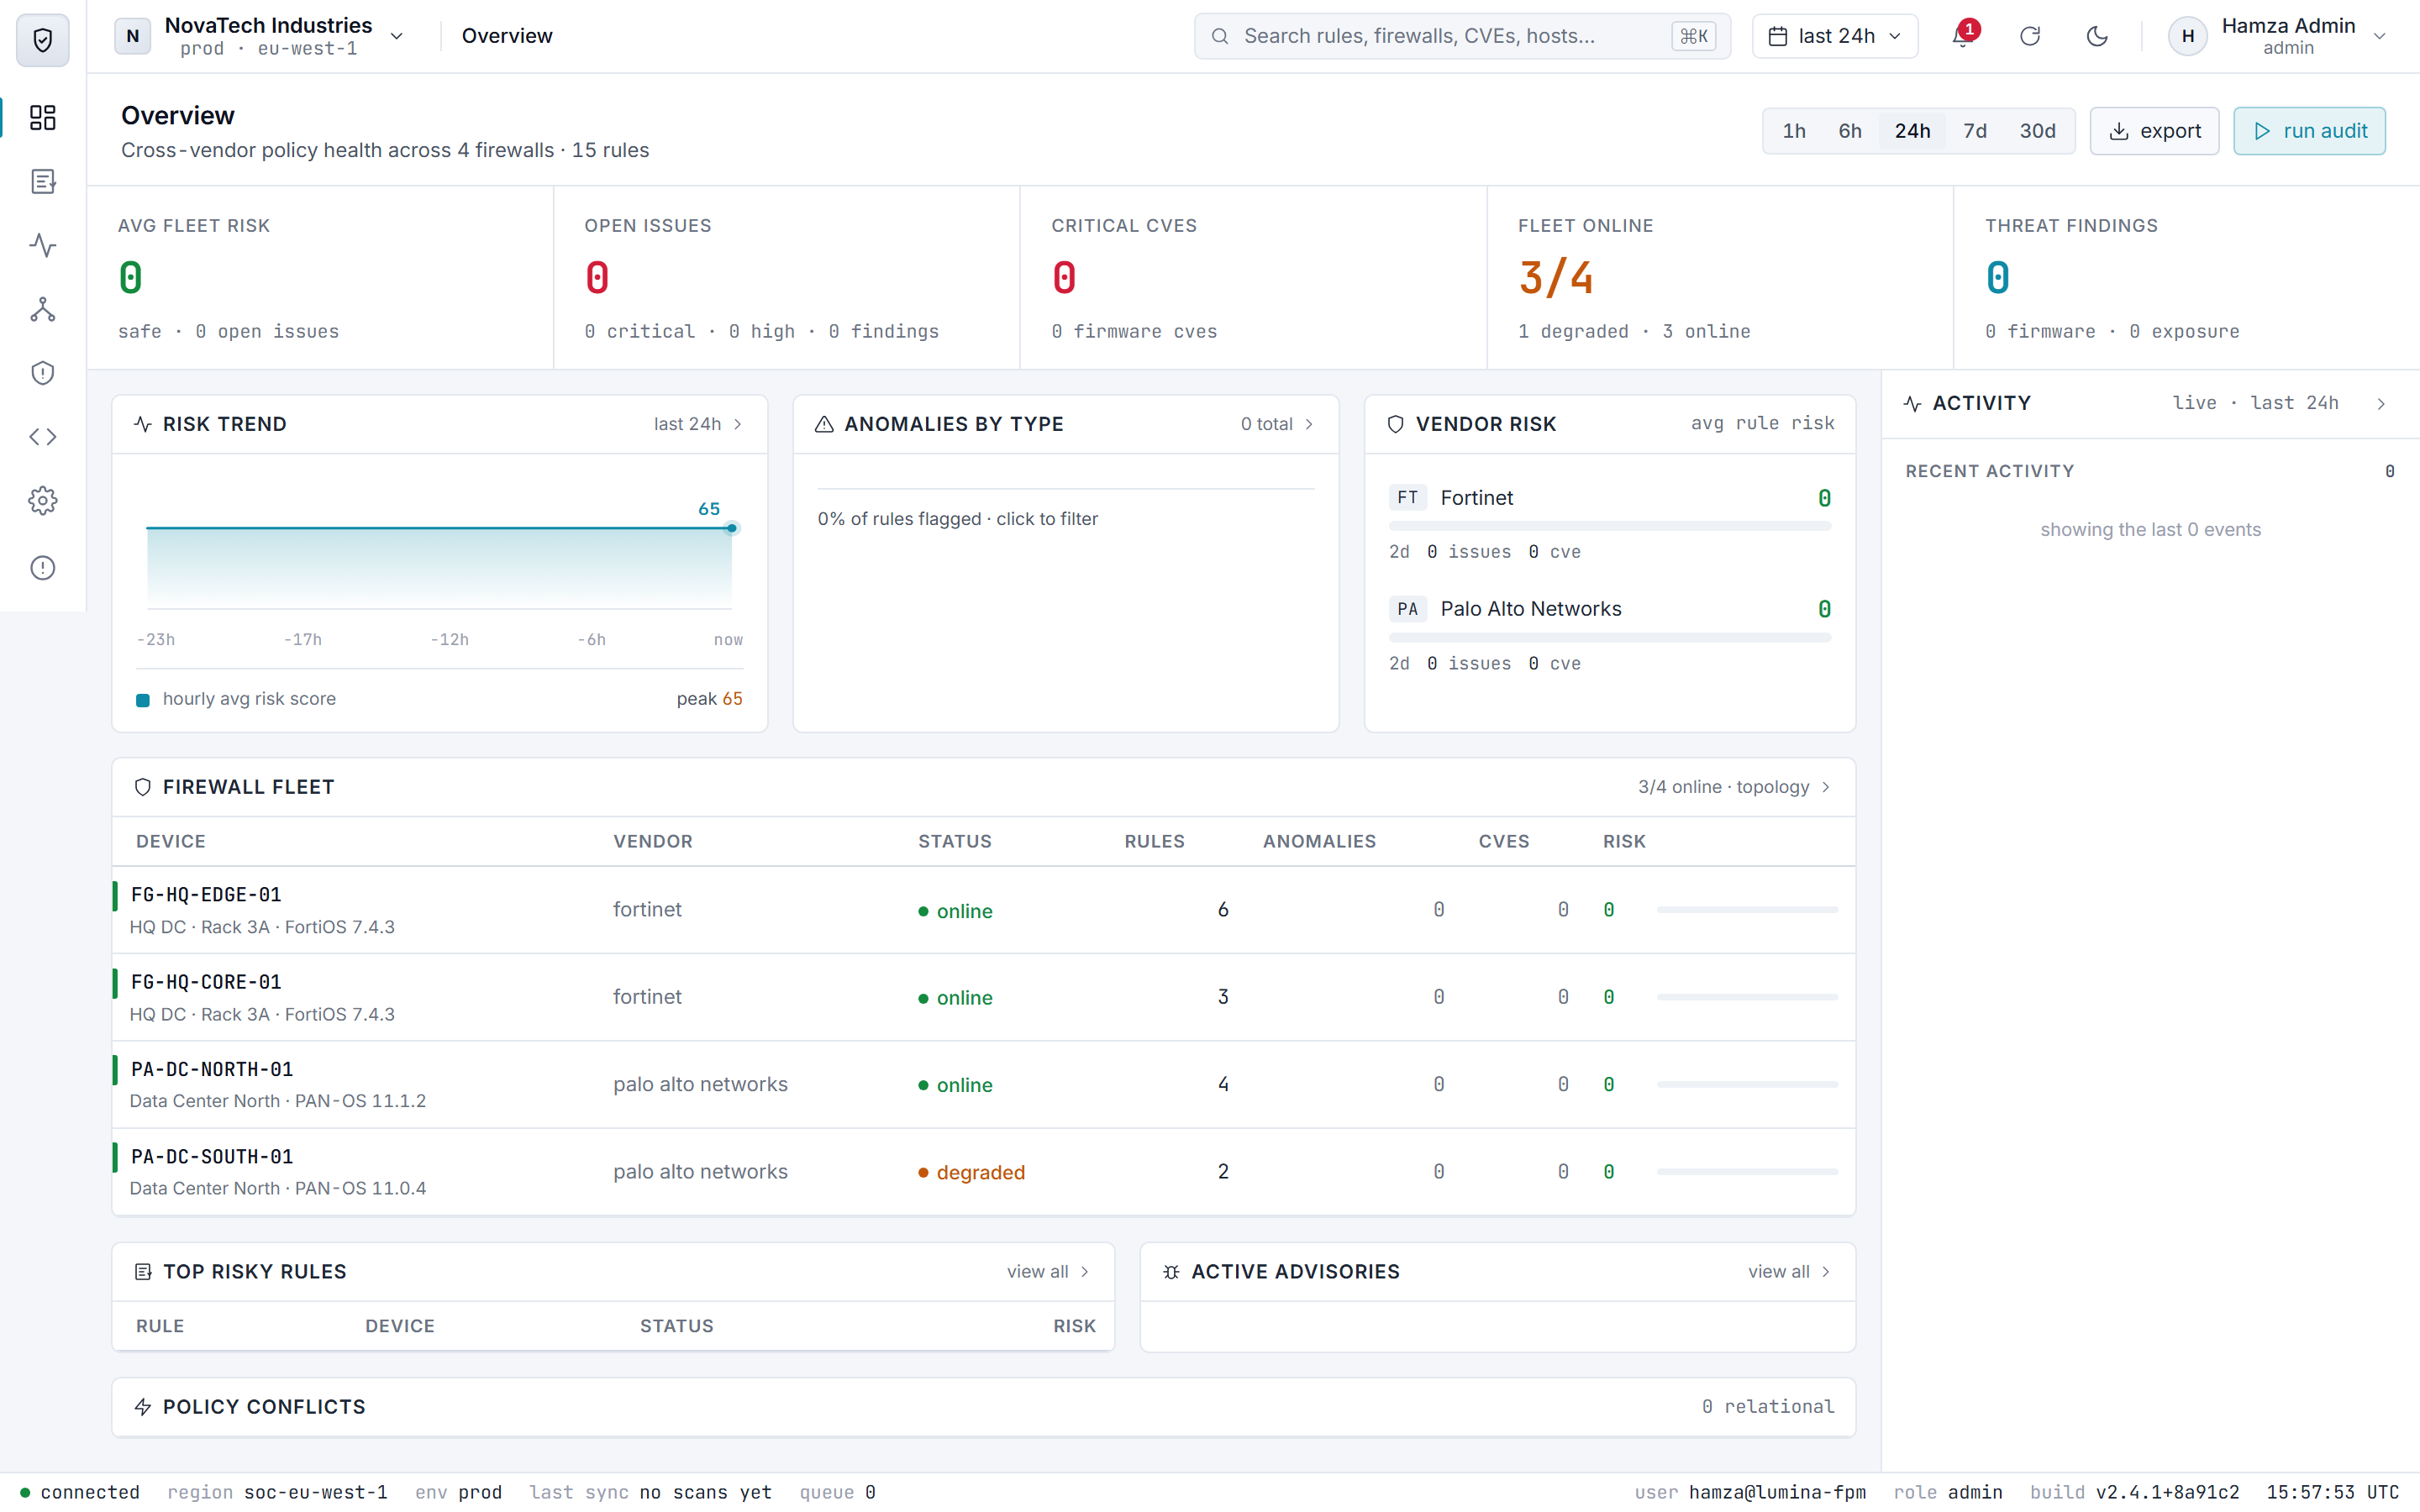
\includegraphics[width=0.97\linewidth]{figures/ui-dashboard.png}}
\caption{LuminaFPM dashboard (overview).}\label{fig:ui-dashboard}
\end{figure}

The \textbf{Policy Audit} screen (Figure~\ref{fig:ui-audit}) is the analyst's primary workspace. It lists run-scoped, per-rule anomalies with severity-based status and real V8 risk, offers faceted filters (saved views, severity, vendor, firewall, action, a minimum-risk slider), sortable columns, CSV export, and deep-link intent application. A row click opens the slide-over \textbf{Inspector}, whose \texttt{AnomalyCard} exposes the analyst lifecycle (\emph{resolve} / \emph{false\_positive} / \emph{accept\_risk}), each issuing a \texttt{PATCH /anomalies/\{id\}} with a prompted reason where required.

\begin{figure}[htbp]
\centering
\fbox{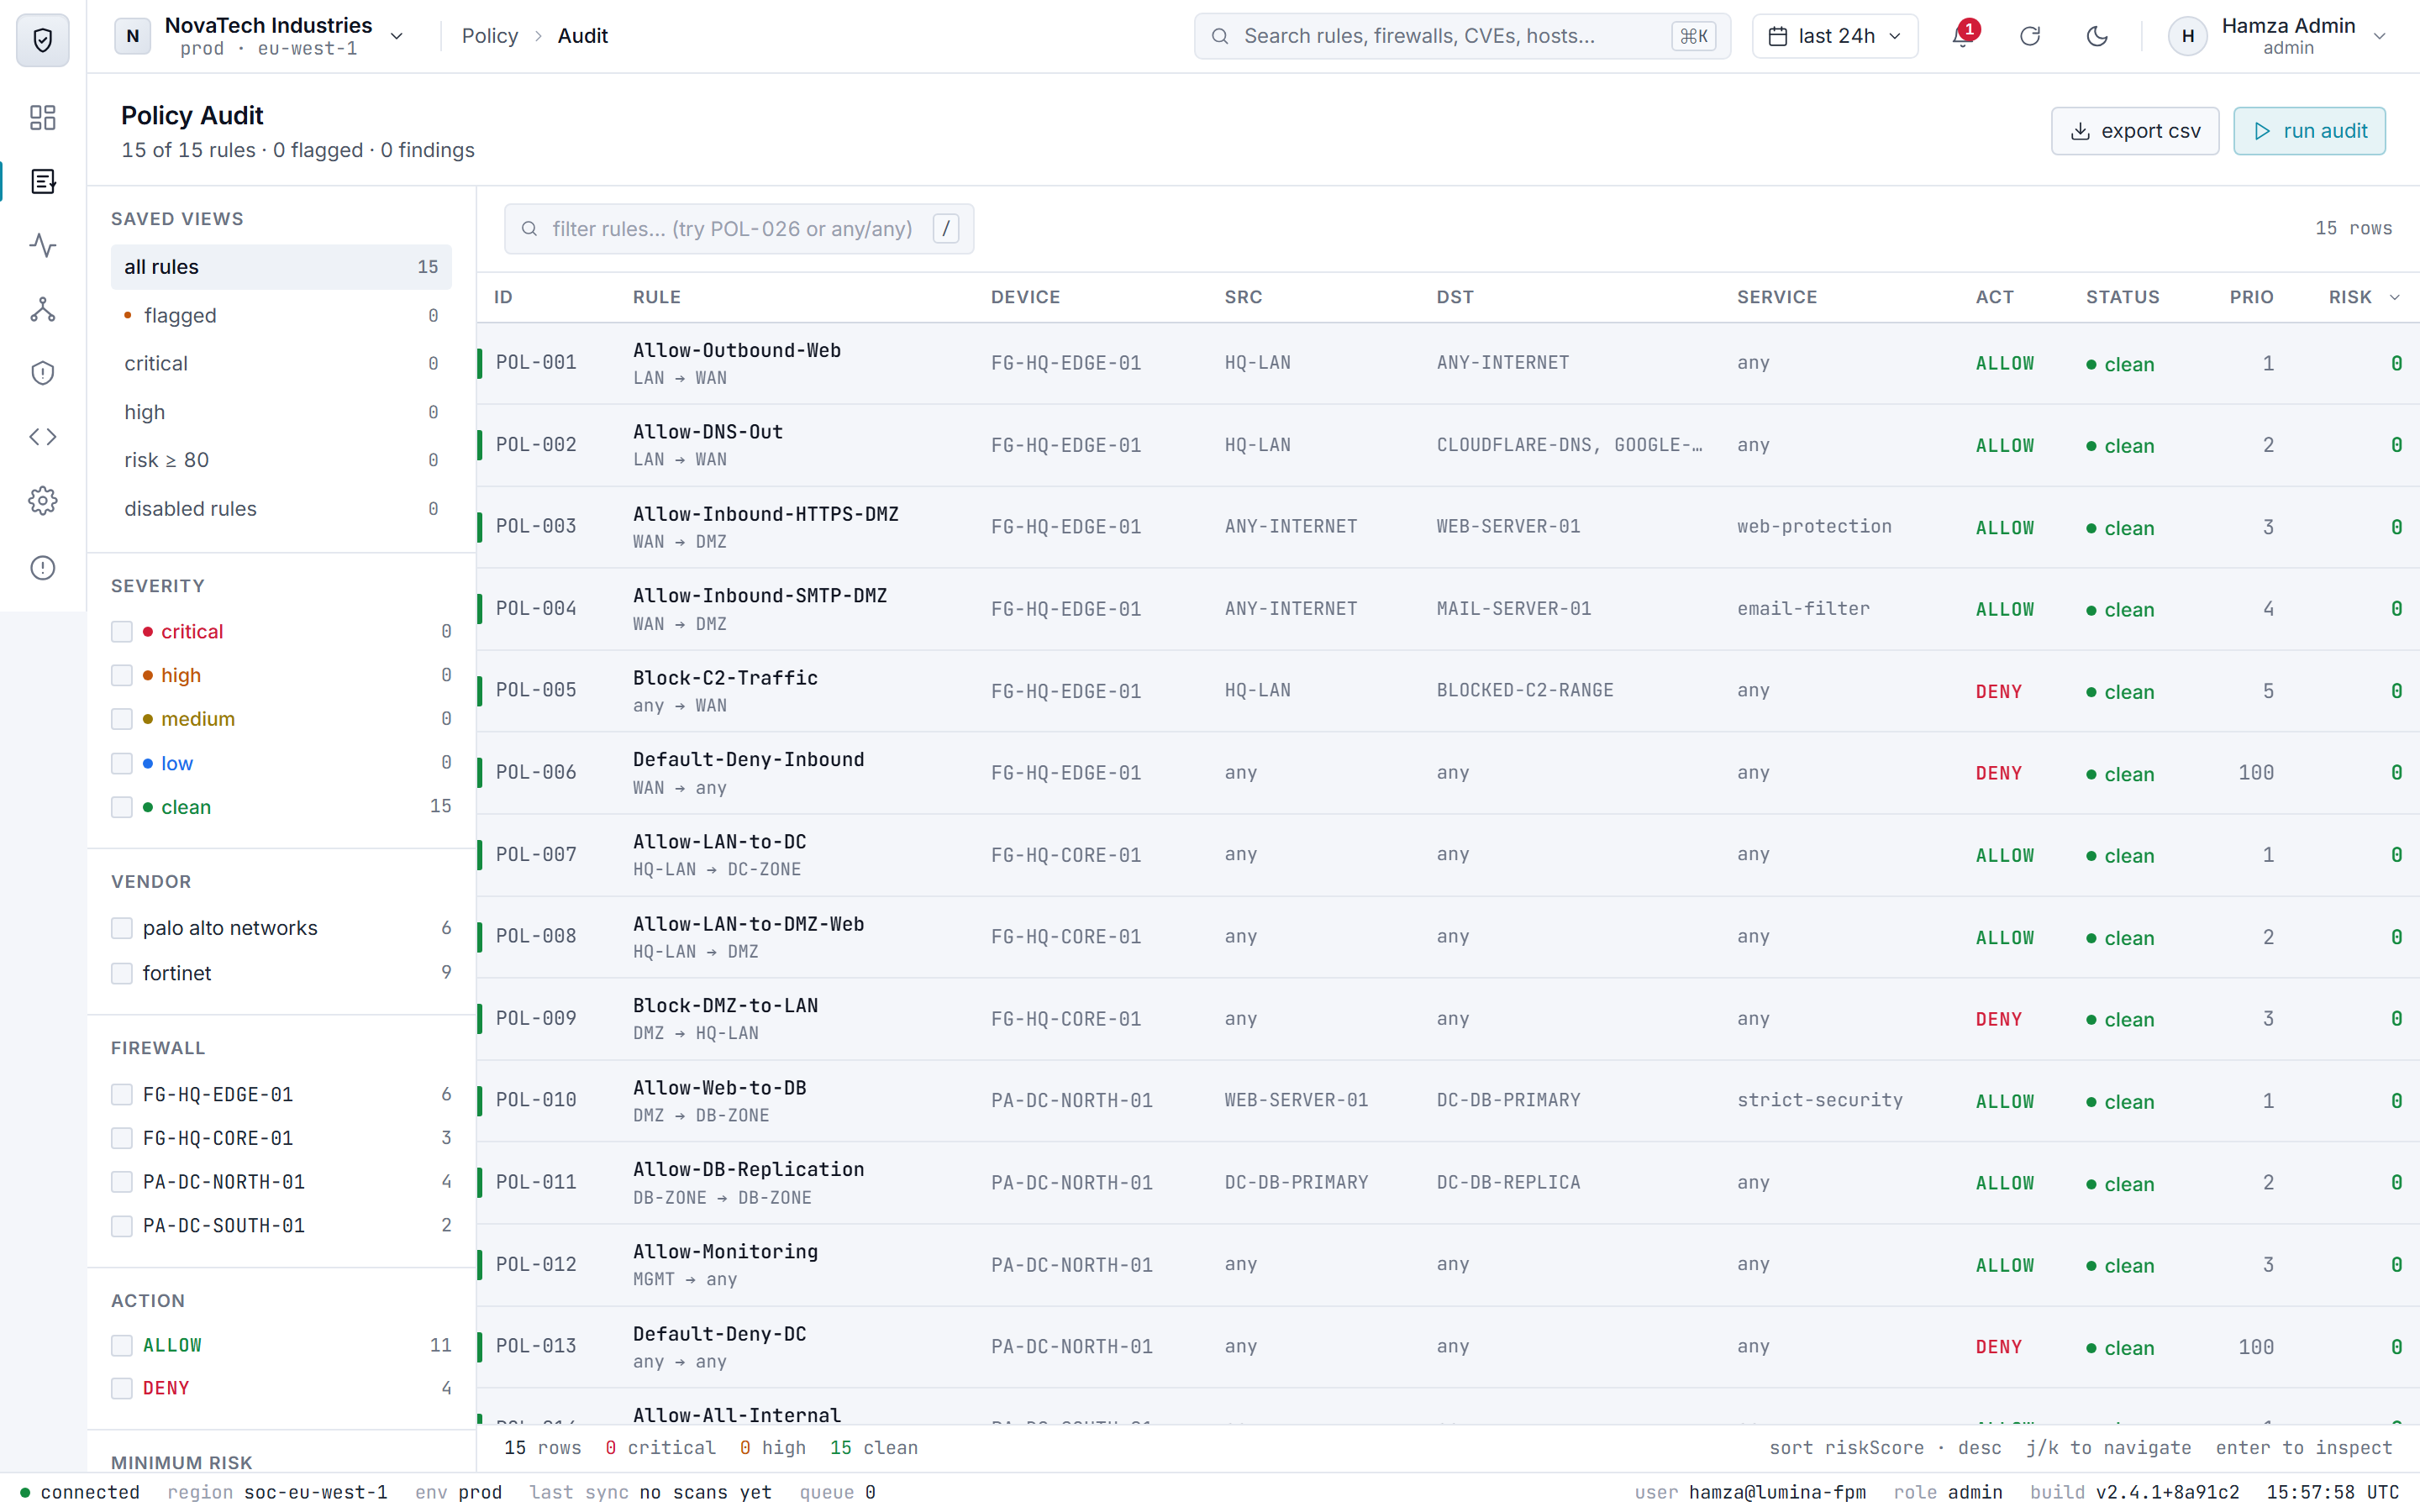
\includegraphics[width=0.97\linewidth]{figures/ui-audit.png}}
\caption{LuminaFPM policy audit and rule inspector.}\label{fig:ui-audit}
\end{figure}

The \textbf{Risk Posture}, \textbf{SOC Reports}, and \textbf{CTI / Threat Center} screens are the typed (\texttt{.tsx}) surfaces. Risk Posture renders device-risk cards and a top-risky-rules table with \texttt{factor\_breakdown} chips and the tier legend. SOC Reports (Figure~\ref{fig:ui-reports}) drives \texttt{reports.generate}/\texttt{list}/\texttt{get}, rendering the LLM output through a dependency-free markdown renderer alongside its \texttt{evidence\_refs} and \texttt{confidence\_note}, and gracefully handling the \texttt{failed} status when no provider is configured. The CTI Center renders the indicator table (provider verdict, threat type, confidence) joined to the affected ALLOW rules from \texttt{threat\_exposure} anomalies.

\begin{figure}[htbp]
\centering
\fbox{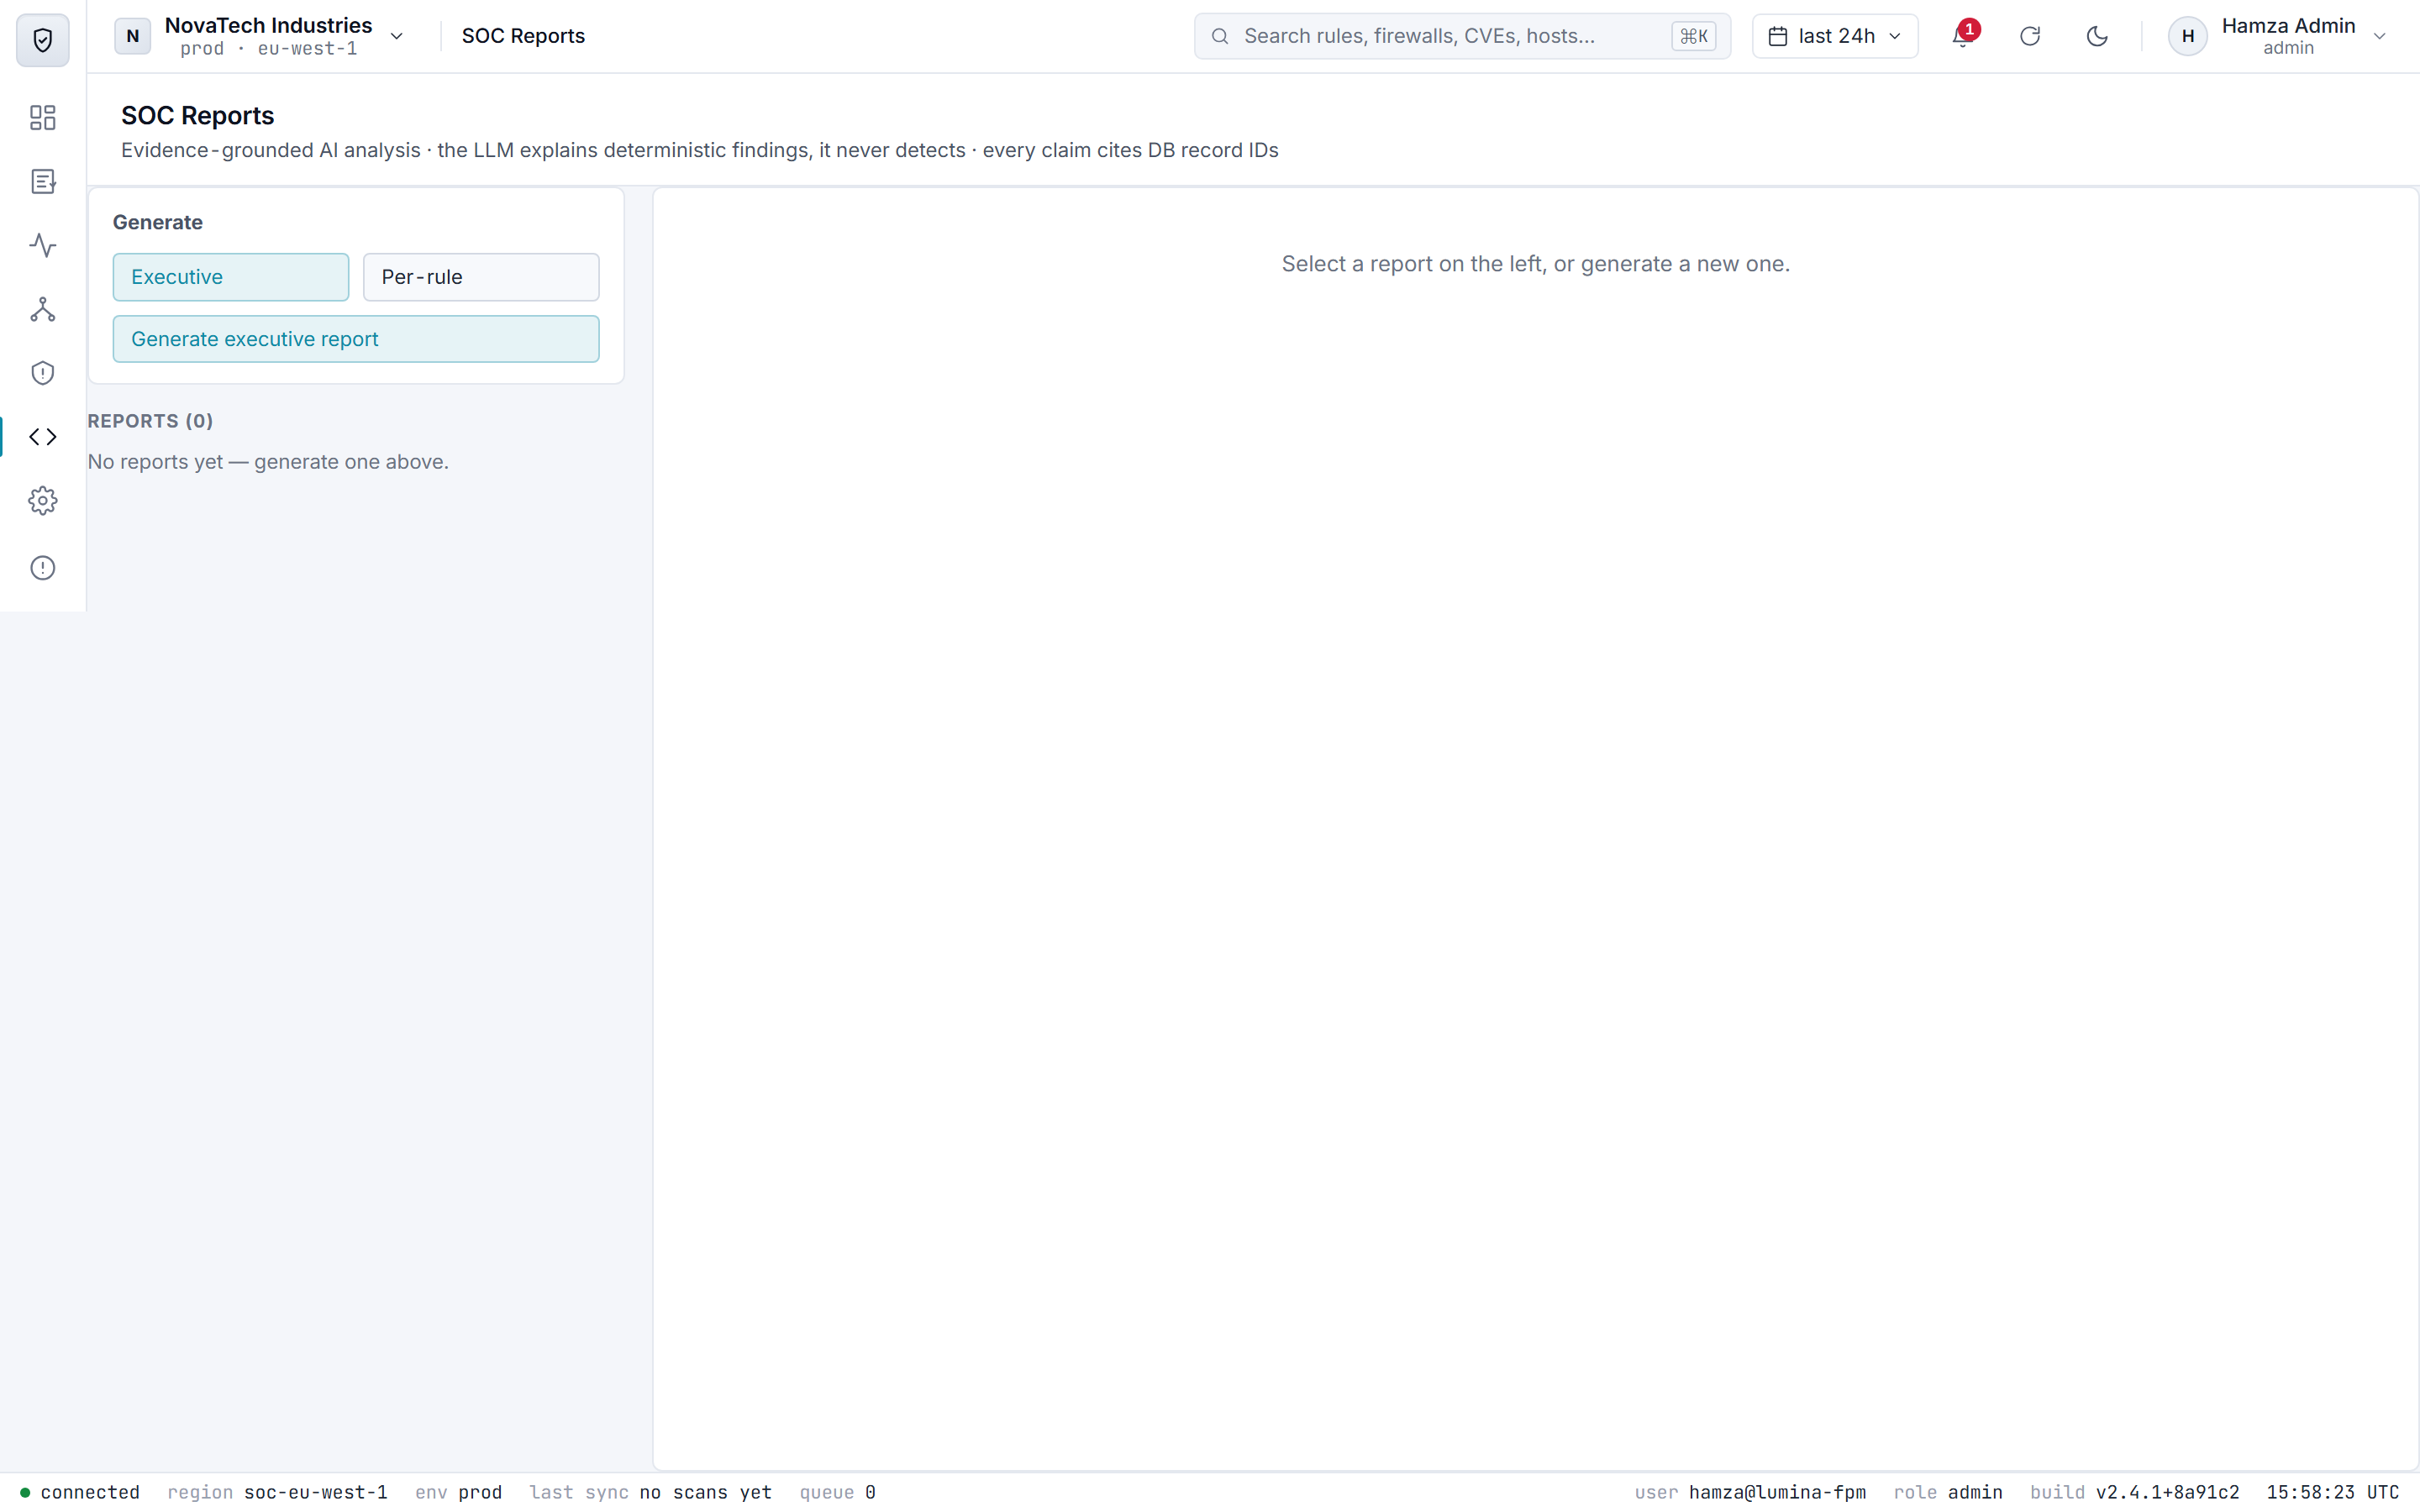
\includegraphics[width=0.97\linewidth]{figures/ui-reports.png}}
\caption{LuminaFPM AI-assisted SOC report viewer.}\label{fig:ui-reports}
\end{figure}

The \textbf{Topology} screen (Figure~\ref{fig:ui-topology}) visualizes the fleet --- firewalls, zones, monitored assets, and CTI threat vectors --- as an \emph{interactive} graph built on Cytoscape.js. It uses a vendor-lane compound layout (each firewall is a lane containing its zone stacks and monitored assets), with draggable nodes whose positions persist to \texttt{localStorage}, wheel-zoom and pan, a live firmware-CVE badge sourced from each device's acquired \texttt{firmware\_version}, PNG export, and the \texttt{?device=} deep-link; clicking any node opens the Inspector with the firewall, zone, host, external-indicator, or path payload. The \textbf{Benchmark Center} surfaces the acceptance gate (Part~B) as a first-class screen, running \texttt{benchmark.run} then \texttt{benchmark.report} and displaying precision/recall/$F_1$, severity-match, the TP/FP/FN counts, per-type coverage, and a per-case matrix. The \textbf{Threat Center} presents the two CTI axes side by side: the \emph{indicator} axis lists enriched indicators (provider verdict, threat type, confidence) joined to the ALLOW rules they expose through \texttt{threat\_exposure} findings, while the \emph{firmware-CVE} axis lists each device's installed firmware and the CVEs that firmware matches. \textbf{Settings} is a functional administrative console: its \emph{Firewalls} tab performs full device management toward the platform's own database --- add, edit, delete, set or rotate the encrypted credential, test the connection, and trigger an acquisition --- while remaining strictly read-only toward the firewalls themselves; its \emph{Scheduling} tab configures interval or cron schedules for acquisition, detection, and threat intelligence with an immediate run-now action; and its \emph{Notifications} tab shows the in-app notification feed. The remaining tabs (access and roles, API and secrets, audit log) are descriptive placeholders pending the authentication work described in Future Work.

\begin{figure}[htbp]
\centering
\fbox{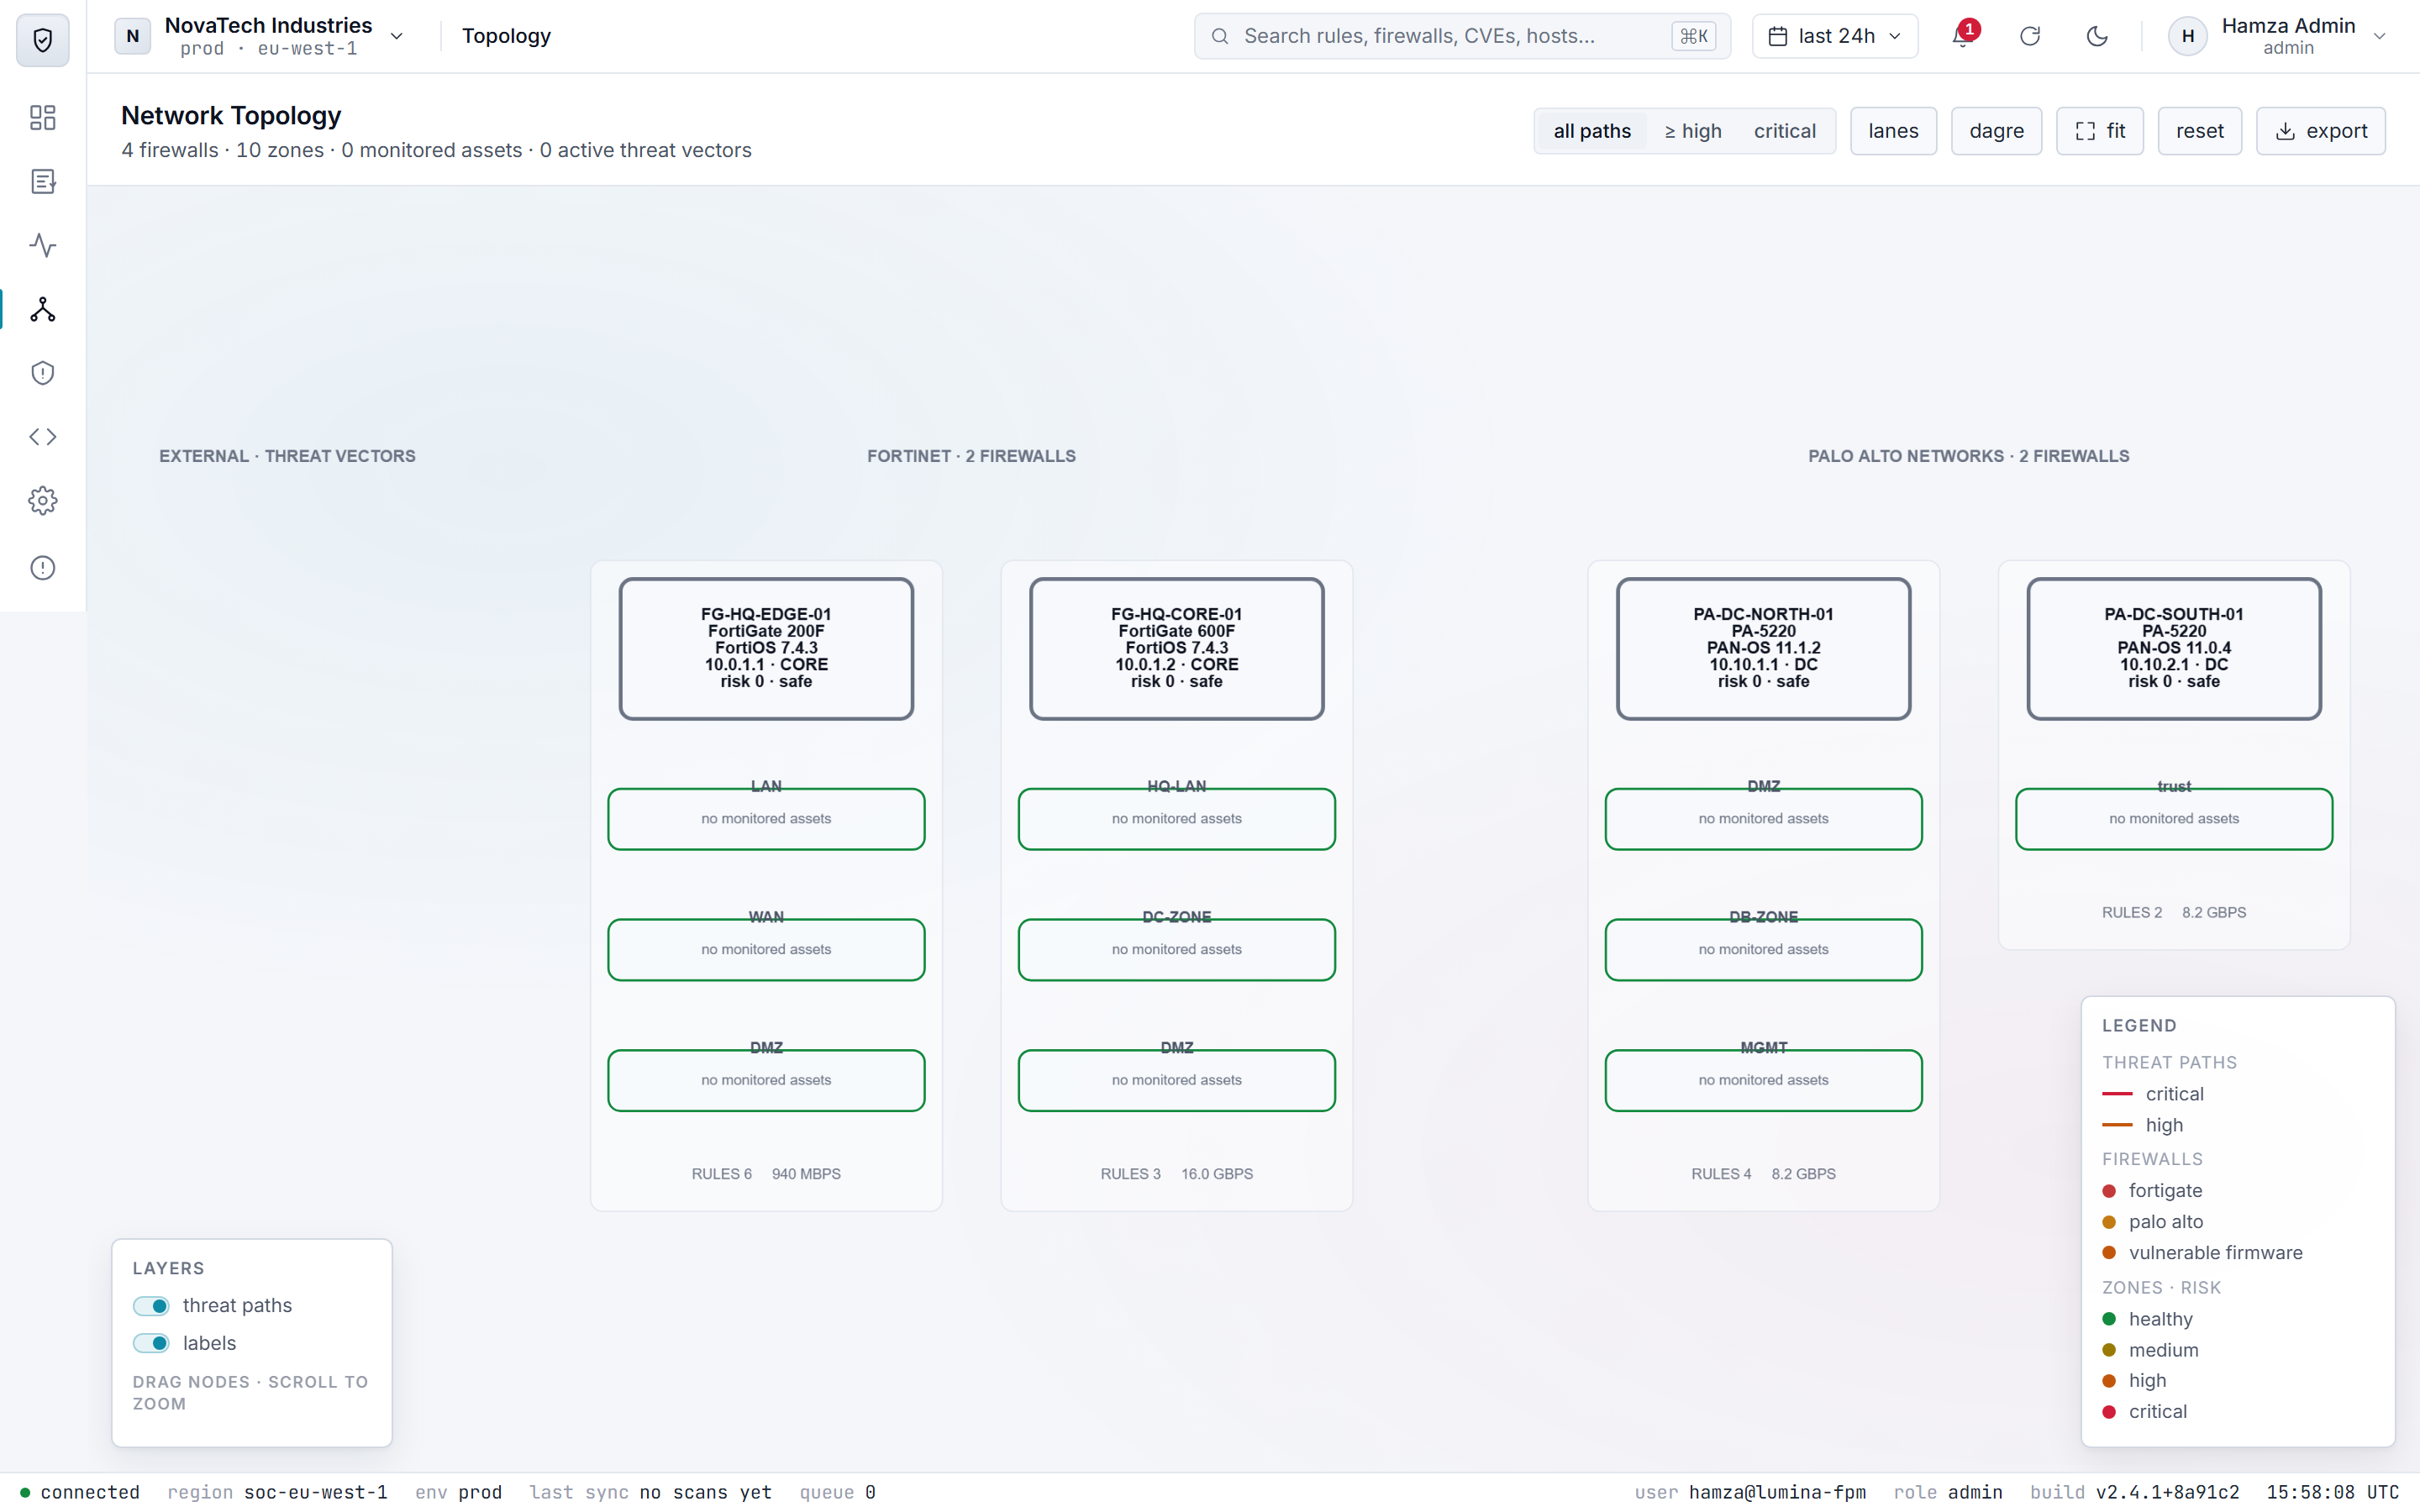
\includegraphics[width=0.97\linewidth]{figures/ui-topology.png}}
\caption{LuminaFPM logical policy topology.}\label{fig:ui-topology}
\end{figure}

Several divergences are documented plainly rather than hidden: the login screen is a cosmetic mock with no backend authentication route, and the API route handlers enforce no per-endpoint authorization (RBAC is specified but not yet wired into the routers); a handful of Cisco/ASA code paths remain dormant though v1 supports FortiGate and Palo Alto only; and a few installed front-end dependencies (\texttt{recharts} and \texttt{react-router-dom}) are present but unused because the corresponding features --- charts and routing --- are deliberately hand-rolled (Cytoscape.js, by contrast, is now used by the topology). These are recorded as known states and candidates for cleanup, consistent with the project's commitment to honest documentation.


\section{Settings, Scheduling, and Notifications}
\label{sec:ch4-settings}

A late addition to the platform turns the \emph{Settings} screen from a descriptive placeholder into a functional administrative console, and adds two supporting subsystems --- scheduling and in-app notifications --- that operationalize the pipeline. All three are built strictly within the project's read-only-against-firewalls mandate: every mutation they perform targets LuminaFPM's own database, never a vendor device.

The \emph{Firewalls} tab performs full device lifecycle management against the platform's own database: it can create, edit, and delete devices, set or rotate each device's Fernet-encrypted credential, and trigger an acquisition, while remaining strictly read-only toward the firewalls themselves. The credential is write-only --- it is encrypted at rest and never returned by the API --- and the only outbound operation is a read-only \texttt{test-connection} that authenticates and validates reachability without modifying any vendor state. A new per-device \texttt{use\_http} column on \texttt{firewall\_device} provides a lab HTTP escape hatch for the FortiGate appliance whose HTTPS stack is broken. The tab can onboard a device against an empty database --- the user interface find-or-creates the owning vendor --- so the platform bootstraps cleanly from a clean install.

\begin{figure}[htbp]
\centering
\fbox{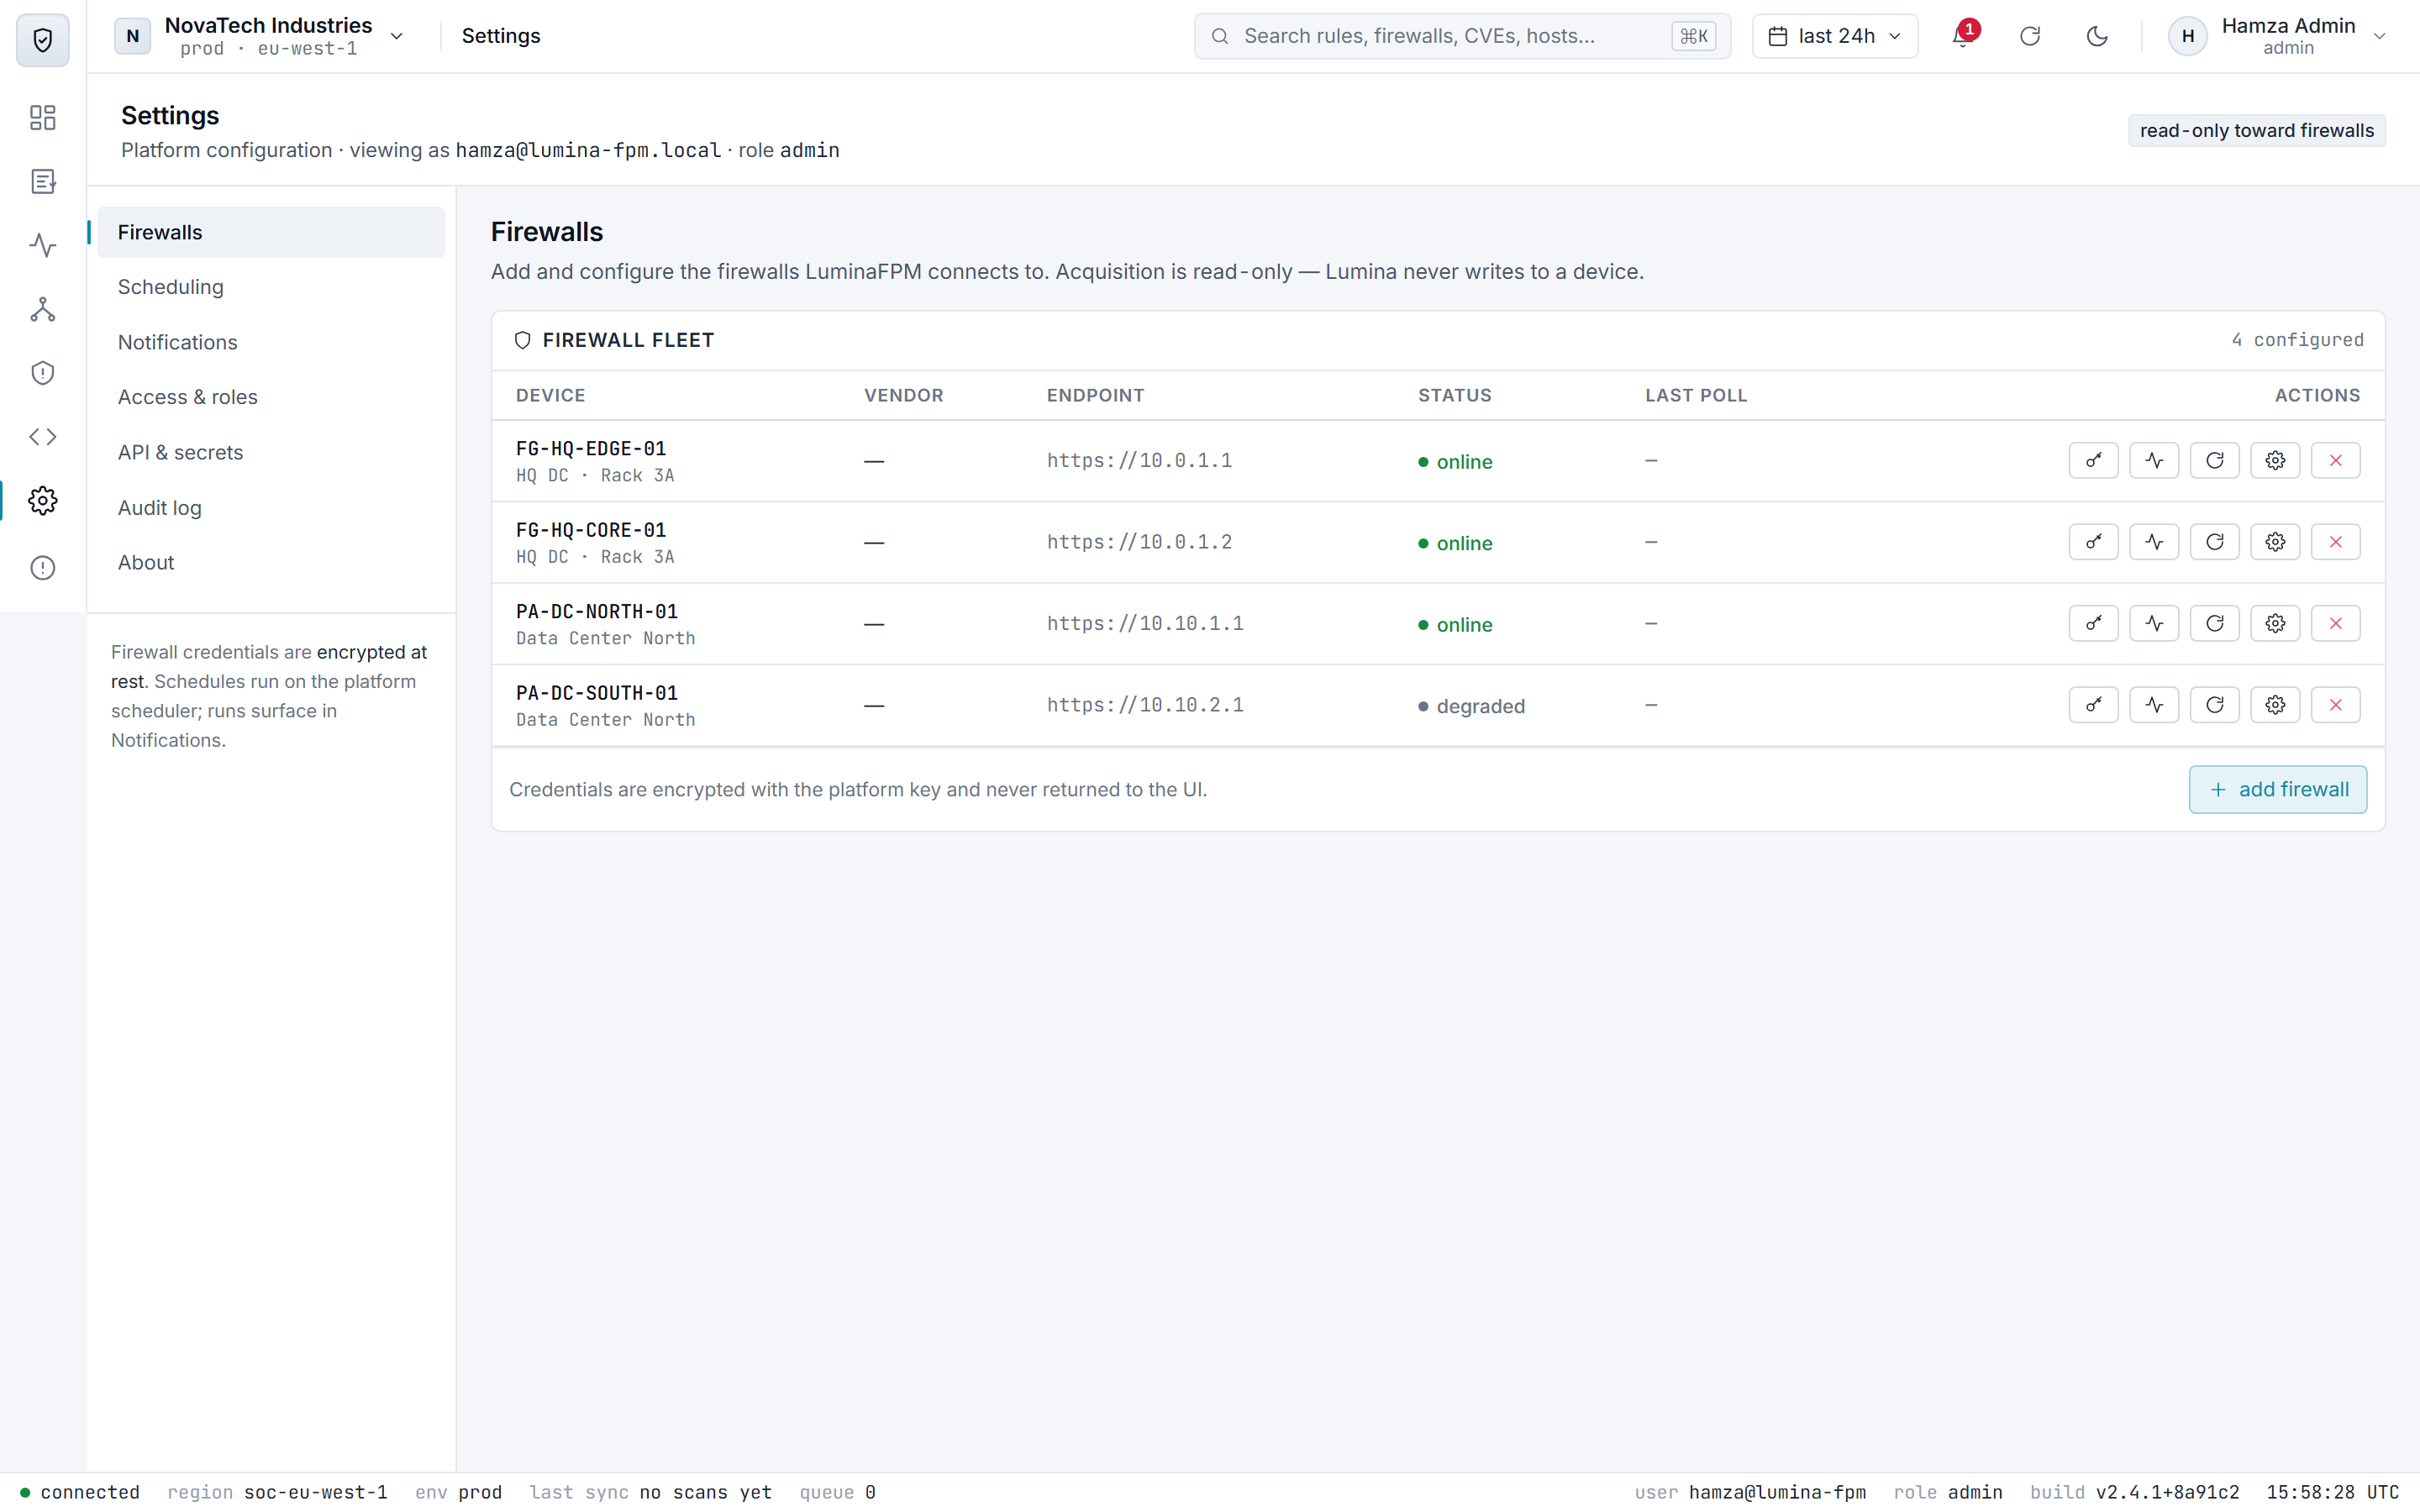
\includegraphics[width=0.97\linewidth]{figures/ui-settings.png}}
\caption{The functional Settings console: the \emph{Firewalls} tab manages the device fleet (add, edit, delete, set/rotate the encrypted credential, test connection, and acquire) while remaining strictly read-only toward the firewalls; the \emph{Scheduling} and \emph{Notifications} tabs sit alongside.}
\label{fig:ui-settings}
\end{figure}

Scheduling is backed by a new \texttt{schedule\_config} table holding one row per operation (\texttt{acquisition}, \texttt{detection}, and \texttt{threat\_intel}), a dependency-free five-field cron evaluator (\texttt{services/scheduling.py}), and a Celery Beat task, \texttt{scheduler.tick}, that fires every 60 seconds, reads the editable table, and dispatches any operation whose next run is due. Each operation can be run immediately (run-now) or on a fixed interval or cron schedule. The control surface is exposed through \texttt{GET /api/v1/schedules}, \texttt{PATCH /api/v1/schedules/\{operation\}}, and \texttt{POST /api/v1/schedules/\{operation\}/run-now}.

In-app notifications are persisted in a new \texttt{notification} table. The pipeline emits a notification on the completion or failure of each major operation (acquisition, detection, and threat-intel) and on every high- or critical-severity finding; emission goes through an \texttt{emit\_safe} helper so that a notification failure can never break the pipeline. The top-bar bell polls the unread count and exposes the feed through \texttt{GET /api/v1/notifications}, \texttt{POST /api/v1/notifications/\{id\}/read}, and \texttt{POST /api/v1/notifications/read-all}. Consistent with the read-only mandate, none of this scheduling or notification machinery ever writes to a firewall.

\section{Testing and Evaluation Strategy}
\label{sec:ch4-testing-strategy}

LuminaFPM is validated through a deliberately layered evaluation strategy, mirroring the discipline that the platform itself enforces on firewall policy: each claim about correctness must be grounded in concrete, reproducible evidence rather than visual inspection. Three complementary layers are used, ordered from the most isolated to the most realistic:

\begin{enumerate}[leftmargin=1.4em]
  \item \textbf{Unit testing} of every backend subsystem in isolation (\path{backend/tests/test_*.py}) --- acquisition, parsing, normalization, anomaly detection, risk scoring, benchmark scoring, CTI and LLM reporting. These tests are pure: by design they run with no live firewall, no network, and no database, using either fixture data captured from the real lab or monkey-patched provider responses. This makes the suite fast, deterministic and runnable on any developer machine as a regression gate.
  \item \textbf{Deterministic benchmark evaluation} against an authoritative ground-truth matrix (Volume~7; \path{backend/services/benchmark/}). This is the platform's \emph{acceptance gate}: the deterministic anomaly engine is scored against an expected-anomaly matrix, producing true/false-positive and false-negative counts and the derived precision, recall, $F_1$ and severity-match metrics. The benchmark proves the engine works against a known answer key rather than against the analyst's intuition.
  \item \textbf{Live end-to-end validation} on the parallel VMware lab, against the real Fortinet FortiGate (\texttt{192.168.55.10}) and Palo Alto PAN-OS (\texttt{192.168.55.20}) devices on \texttt{192.168.55.0/24}. The full pipeline --- poll $\rightarrow$ parse $\rightarrow$ normalize $\rightarrow$ analyze $\rightarrow$ risk $\rightarrow$ CTI $\rightarrow$ report --- is executed against live vendor configuration, exercising the connectors, the cross-vendor correlation, and the persistence layer that the pure unit tests deliberately stub out.
\end{enumerate}

The three layers are intentionally redundant in coverage but distinct in fidelity. Unit tests catch logic regressions cheaply; the benchmark proves the engine's \emph{output} matches a per-type ground truth with measurable precision and recall; and the live run proves the same code path survives contact with real vendor APIs, real self-signed certificates, and real multi-vendor configuration drift. A defect surfaced at a higher layer is, wherever possible, pushed back down into a unit test --- as happened with the FortiGate \texttt{ALL}-service normalization defect (Section~\ref{sec:ch4-findings}), which was first observed in a live run and then permanently captured as a normalization regression test.

\section{Unit Testing}
\label{sec:ch4-unit-testing}

The backend unit suite lives under \path{backend/tests/} and comprises eleven subsystem test files. Each is structured to exercise the \emph{pure} core of its subsystem --- the scoring, parsing, or detection logic that contains no I/O --- so that correctness is asserted independently of the database-backed runners that persist results. Where real vendor data is required, the suite uses fixtures captured directly from the lab firewalls (e.g.\ \path{backend/tests/fixtures/fortigate_policy.json} and \path{paloalto_rulebase.xml}, the genuine FortiOS~v7.0.5 and PAN-OS responses), so the parsers and the normalizer are validated against real-world payload shapes, not synthetic mock-ups. Table~\ref{tab:ch4-unit-tests} summarizes the coverage of each file.

{\small
\begin{longtable}{L{3.8cm}L{10.8cm}}
\caption{Backend unit-test coverage by subsystem (\texttt{backend/tests/}).}
\label{tab:ch4-unit-tests}\\
\hline
\hcell{Test file} & \hcell{Subsystem and what is asserted} \\
\hline
\endfirsthead
\hline
\hcell{Test file} & \hcell{Subsystem and what is asserted} \\
\hline
\endhead
\hline
\endfoot
\hline
\endlastfoot
\texttt{test\_acquisition.py} & Read-only connectors and raw-artifact storage. Monkey-patched FortiOS JSON and PAN-OS XML responses; firmware extraction (FortiGate v7.4.1, Palo Alto 11.1.3); partial-success behaviour on an optional-endpoint 404; raw-artifact manifest with per-artifact SHA-256 and replay. No network or DB required. \\
\texttt{test\_parsing.py} & Vendor parsers against \emph{real captured lab artifacts} (FortiOS v7.0.5, PAN-OS). Asserts both vendors parse to a uniform \texttt{ParsedDevicePayload} and that the cross-device benchmark pair (LAN\_NET$\rightarrow$WEB\_SERVER, HTTPS, allow, no inspection) is equivalent at the parse level. \\
\texttt{test\_normalization.py} & The cross-vendor normalization keystone. Asserts that the FortiGate and Palo Alto definitions of \texttt{LAN\_NET} (10.10.10.0/24) and \texttt{WEB\_SERVER} (10.10.20.10/32) correlate to a single canonical object each (confidence 1.00), that PAN's predefined \texttt{service-https} resolves to the same \texttt{tcp/443} canonical service as FortiGate's custom HTTPS, and that repeated runs produce identical content hashes (determinism). \\
\texttt{test\_anomaly.py} & The deterministic anomaly engine. Ground-truth assertions on the real fixtures (exactly two \texttt{unprotected\_allow} and two \texttt{missing\_description}, and \emph{no} false cross-device finding) plus crafted unit tests for \texttt{shadowing}, \texttt{duplicate\_rules}, \texttt{conflict}, \texttt{any\_to\_sensitive} and \texttt{overly\_permissive}; includes the FortiGate \texttt{ALL}-service shadowing/redundancy regression. \\
\texttt{test\_risk.py} & The pure risk scorer (Volume~8): \texttt{tier\_of} band boundaries, \texttt{score\_rule} factor derivation, the clean$\rightarrow$\emph{informational} and governance$\rightarrow$\emph{low} cases, the broad-unprotected-unlogged$\rightarrow$\emph{critical} case, the cross-device \texttt{cross\_vendor} factor, the cap at 100, and the \texttt{score\_device} top-5 blend. \\
\texttt{test\_benchmark.py} & The pure benchmark scorer (Volume~7): a perfect-match case, a false negative driving recall down, a false positive driving precision down, a cross-device pair matched on either side, and a severity mismatch driving the severity-match rate down. \\
\texttt{test\_cti.py} & v1 API-based CTI (Volume~9): \texttt{is\_public\_ip}/\texttt{classify}/\texttt{extract\_indicators} with RFC1918 data-minimization, the deterministic \texttt{LabOfflineProvider} verdict, the provider registry, and the \texttt{threat\_exposure}$\rightarrow$CTI risk-factor path (+28). \\
\texttt{test\_llm.py} & v1 LLM SOC reporting (Volume~10): the guardrail \texttt{SYSTEM\_PROMPT} (``use only evidence'', ``do not invent'', ``the deterministic engine --- not you --- decides''), \texttt{OfflineProvider} determinism, provider fallback when unkeyed, and evidence-ID embedding in the rendered prompt. \\
\texttt{test\_benchmark\_matrix.py} & The offline engine acceptance gate. Inlines the enriched 26-rule matrix (10 FortiGate + 16 Palo Alto) and asserts the deterministic engine reproduces the ground-truth answer key exactly --- 43 expected cases, 0 false positives, 0 false negatives, 0 severity mismatches --- before any device is provisioned, so a detection regression fails the suite without a live lab. \\
\texttt{test\_vuln.py} & The firmware-CVE device axis (Volume~9). Version-tuple and affected-range parsing, CVSS-to-severity banding, the offline lab CVE dataset (Fortinet and Palo Alto only --- Cisco-free), the device-affected predicate, and the firmware modifier that raises device risk. \\
\texttt{test\_scheduling.py} & The dependency-free five-field cron engine behind the Settings scheduler. Field parsing with range/step/list validation, match evaluation (daily, step, day-of-week), and the next-run computation that drives Celery Beat. \\
\hline
\end{longtable}
}

The optional Lumina-Threat-Intel (LTI) module carries its own separate tests under \path{backend/services/lumina_threat_intel/tests/} (diff-tracker hashing, the LLM-client JSON extraction and retry path, and prompt anti-hallucination checks); these are not part of the v1 acceptance suite and are documented only for completeness. The eleven v1 files above constitute the regression gate that must pass before any live run.

\section{Benchmark Evaluation (Acceptance Gate)}
\label{sec:ch4-benchmark}

The benchmark framework (Volume~7; \path{backend/services/benchmark/scorer.py}, \texttt{ground\_truth.py}, \texttt{runner.py}) is the formal acceptance gate for the detection engine. Its premise is that an anomaly engine cannot be trusted on the strength of plausible-looking output; it must be scored against an answer key constructed independently of the engine itself.

\subsection{Metrics: TP / FP / FN and the derived rates}

The pure scorer (\texttt{scorer.py}) compares the engine's actual findings for an analysis run against an \texttt{ExpectedCase} matrix. Matching granularity is \emph{(rule, anomaly\_type) presence} --- not a count --- so a rule that is expected to exhibit a given anomaly type counts once. For a cross-device case the anomaly may legitimately appear on \emph{either} of the two paired rules, because the engine attributes a cross-device finding to one side; such a case matches if the type is present on either rule. From the comparison the scorer computes:

\begin{itemize}[leftmargin=1.4em]
  \item \textbf{True positives (TP)} --- expected cases the engine detected.
  \item \textbf{False negatives (FN)} --- expected cases the engine missed.
  \item \textbf{False positives (FP)} --- reported \texttt{(rule, anomaly\_type)} pairs that no expected case consumed.
  \item \textbf{Precision} $= \mathrm{TP}/(\mathrm{TP}+\mathrm{FP})$, \textbf{recall} $= \mathrm{TP}/(\mathrm{TP}+\mathrm{FN})$, and $F_1 = 2PR/(P+R)$, each guarded against a zero denominator and rounded to four decimal places.
  \item \textbf{Severity-match rate} $=$ (cases whose detected severity equals the expected severity) $/\ \mathrm{TP}$. Because the expected severity is fixed per anomaly \emph{type} (Volume~6 Table~7) and is independent of the engine, this rate is a genuine, separate check that the engine assigns the correct severity, not merely the correct type.
\end{itemize}

\subsection{Ground-truth construction}

The expected matrix is authored in \path{backend/services/benchmark/ground_truth.py}, which mirrors the design intent of \path{lab/benchmark_dataset.py} but is kept inside the backend because the \texttt{lab/} directory is not mounted into the API container. Each expected anomaly is derived from a rule's \emph{configuration plus the detector definitions} --- never from engine output --- so the matrix is a true answer key. \texttt{EXPECTED\_SEVERITY} pins thirteen anomaly types to a severity (e.g.\ \texttt{any\_to\_sensitive}, \texttt{overly\_permissive} and \texttt{cross\_device\_inconsistency} are \emph{critical}; \texttt{unprotected\_allow}, \texttt{shadowing} and \texttt{conflict} are \emph{high}; \texttt{missing\_description} and \texttt{disabled\_rule\_review} are \emph{low}). The \texttt{INTRA} table maps each named rule, per vendor, to its expected config-only anomalies --- for example \texttt{FGT\_ANY\_ANY} $\rightarrow$ \{\texttt{overly\_permissive}, \texttt{unprotected\_allow}, \texttt{missing\_logging}, \texttt{missing\_description}, \texttt{conflict}\} and \texttt{FGT\_ANY\_DB} $\rightarrow$ \{\texttt{any\_to\_sensitive}, \texttt{unprotected\_allow}, \texttt{missing\_logging}, \texttt{missing\_description}\}. \texttt{CROSS\_DEVICE} enumerates three pairs: one \texttt{cross\_device\_inconsistency} (\texttt{FGT\_DB\_ACCESS\_XDEV} vs \texttt{PA\_DB\_ACCESS\_XDEV} --- the same canonical LAN\_NET$\rightarrow$DB\_SERVER MySQL access where FortiGate allows but Palo Alto denies) and two \texttt{cross\_device\_security\_posture\_inconsistency} pairs (an equivalent LAN$\rightarrow$WEB HTTPS allow that FortiGate inspects but Palo Alto leaves unprotected).

\subsection{Deployment filtering and \texttt{config\_only} scoping}

The runner (\texttt{runner.py}) resolves the matrix only against \emph{deployed} rules: an intra-device case is skipped when its rule is not present in \texttt{policy\_rule}, and a cross-device case is scored only when \emph{both} paired rules are deployed. This is what keeps cap-dropped rules (e.g.\ \texttt{FGT\_ADMIN\_DB\_NOLOG} and \texttt{FGT\_DISABLED\_RISKY}, omitted under the FortiGate-VM ten-policy cap) from being mis-counted as false negatives. Crucially, the runner joins \texttt{RuleAnomaly}$\rightarrow$\texttt{PolicyRule} filtered both by \texttt{analysis\_run\_id} and by \texttt{detection\_mode == "config\_only"}. This filter is what makes the benchmark sound: the configuration-only detectors are scored against the configuration-only answer key, while the \texttt{cti}-mode \texttt{threat\_exposure} finding (which is not a configuration anomaly) is excluded and evaluated separately. The acceptance criterion (Volume~7 Table~7) is qualitative --- every core config-only anomaly detected in atomic cases, both cross-device cases detected, compound findings present, simulated cases labelled, and every finding traceable to its rule(s) and reason --- and the runner exposes the raw metrics rather than hard-coding a numeric $F_1$ threshold.

\section{Test Cases and Outputs}
\label{sec:ch4-test-cases}

This section presents concrete test cases and their outputs from the live lab, focused on the canonical end-to-end run, \textbf{analysis run~\#25}, executed against both vendors. It proceeds from individual rule-level cases, through the aggregate run output, to the benchmark scorecard and the CTI and AI-reporting cases.

\subsection{Representative rule-level cases}

Table~\ref{tab:ch4-rule-cases} lists representative policy rules deployed on the lab firewalls and the anomalies the deterministic engine produced for each. Every entry is reproducible: the rule is read from live vendor configuration, normalized to the canonical model, and evaluated by the fixed-order detector chain, so the same input always yields the same findings.

{\footnotesize
\begin{xltabular}{\linewidth}{L{2.6cm} C{1.0cm} X}
\caption{Representative live rule-level test cases and the engine's findings (run~\#25).}
\label{tab:ch4-rule-cases}\\
\hline
\hcell{Rule} & \hcell{Dev.} & \hcell{Engine findings (anomaly\_type)} \\
\hline
\endfirsthead
\hline
\hcell{Rule} & \hcell{Dev.} & \hcell{Engine findings (anomaly\_type)} \\
\hline
\endhead
\hline
\endfoot
\texttt{FGT\_ANY\_ANY} & FGT & \texttt{overly\_permissive}, \texttt{unprotected\_allow}, \texttt{missing\_logging}, \texttt{missing\_description}, \texttt{conflict} --- an any/any/any allow with no inspection or logging. \\
\texttt{PA\_ANY\_ANY} & PA & \texttt{overly\_permissive}, \texttt{unprotected\_allow}, \texttt{missing\_logging}, \texttt{missing\_description}, \texttt{conflict} --- the Palo Alto mirror of the above. \\
\texttt{FGT\_ANY\_DB} & FGT & \texttt{any\_to\_sensitive} (ANY source to a \emph{database}-class destination), \texttt{unprotected\_allow}, \texttt{missing\_logging}, \texttt{missing\_description}; plus a separate cti-mode \texttt{threat\_exposure} (its object set references the known-bad indicator --- Section~\ref{sec:ch4-cti-case}). \\
\texttt{PA\_ANY\_DB} & PA & \texttt{any\_to\_sensitive}, \texttt{unprotected\_allow}, \texttt{missing\_logging}, \texttt{missing\_description} --- the Palo Alto mirror. \\
\texttt{FGT\_SHADOWED\_WEB2} & FGT & \texttt{shadowing}, \texttt{conflict} --- preceded by a blocking rule whose canonical sets cover it, so it can never match; the differing action is also flagged as a conflict. \\
\texttt{PA\_SHADOWED\_WEB2} & PA & \texttt{shadowing}, \texttt{conflict} --- the Palo Alto shadowed pair. \\
\texttt{FGT\_REDUNDANT\_WEB} & FGT & \texttt{redundancy}, \texttt{duplicate\_rules} --- a later rule fully covered by an earlier same-action rule. \\
\texttt{FGT\_WIDE\_PORTS} & FGT & \texttt{wide\_port\_range} (a single service spanning $>1024$ ports), \texttt{redundancy}. \\
\texttt{FGT\_DB\_ACCESS\_XDEV} / \texttt{PA\_DB\_ACCESS\_XDEV} & FGT, PA & \texttt{cross\_device\_inconsistency} (critical) --- identical canonical LAN\_NET$\rightarrow$DB\_SERVER MySQL access; FortiGate \emph{allows}, Palo Alto \emph{denies}. The keystone cross-vendor finding. \\
\texttt{PA\_ALLOW\_MALICIOUS} & PA & Config-clean (inspected, logged, described, narrow source) --- the engine raises \emph{no} configuration anomaly; only a separate cti-mode \texttt{threat\_exposure} fires because the rule permits traffic to the known-bad indicator (Section~\ref{sec:ch4-cti-case}). \\
\hline
\end{xltabular}}

Three properties are visible in this table and are central to the platform's thesis. First, \emph{compound findings}: a single permissive rule such as \texttt{FGT\_ANY\_ANY} legitimately produces five distinct findings, each with its own evidence and recommendation. Second, \emph{cross-vendor equivalence}: the FortiGate and Palo Alto mirrors produce the same finding sets because detection operates over the normalized model, not vendor syntax. Third, the \texttt{*\_DB\_ACCESS\_XDEV} pair demonstrates the engine's signature capability --- detecting that two different vendors have reached \emph{contradictory access decisions} about the same canonical traffic, an inconsistency no single-vendor tool could surface.

\subsection{Aggregate run output (run \#25)}

The all-scope analysis run aggregated across both devices. The aggregate output is summarized below and the per-type distribution is given in Table~\ref{tab:ch4-type-distribution}.

\begin{itemize}[leftmargin=1.4em]
  \item \textbf{Scope:} 2~devices (FGT-LAB, PA-LAB), 26~active policy rules (FortiGate~10 under the VM cap, Palo Alto~16), evaluated by the fixed-order chain of 14 deterministic detectors.
  \item \textbf{Current findings:} 43~config-only findings scored for the run --- 40 intra-device plus 3 cross-device pair findings (the frontend scopes to the latest completed all-scope run, separating these from the historical anomalies of earlier runs to avoid cross-run inflation).
  \item \textbf{Device risk (Volume~8):} both Palo Alto and FortiGate score~100 (\emph{critical}). The blend is dominated by the worst rules --- \texttt{PA\_ANY\_DB}/\texttt{FGT\_ANY\_DB} score~99 and \texttt{FGT\_ANY\_ANY}/\texttt{PA\_ANY\_ANY} score~98 --- under a top-5 max-weighted blend plus a critical-count modifier; FortiGate's base of~96 is additionally lifted to the ceiling by a firmware-CVE device modifier of $+40$, and Palo Alto (already at~100) carries a $+30$ firmware modifier, reflecting the device CVEs in Section~\ref{sec:ch4-cti}.
\end{itemize}

\begin{longtable}{L{0.40\textwidth} C{0.18\textwidth} C{0.30\textwidth}}
\caption{Anomaly-type distribution and benchmark coverage, run~\#25.}
\label{tab:ch4-type-distribution}\\
\hline
\hcell{anomaly\_type} & \hcell{Count} & \hcell{Detected?} \\
\hline
\endfirsthead
\hline
\hcell{anomaly\_type} & \hcell{Count} & \hcell{Detected?} \\
\hline
\endhead
\hline
\endfoot
\texttt{unprotected\_allow} & 8 & \checkmark \\
\texttt{missing\_description} & 6 & \checkmark \\
\texttt{missing\_logging} & 6 & \checkmark \\
\texttt{conflict} & 5 & \checkmark \\
\texttt{duplicate\_rules} & 3 & \checkmark \\
\texttt{redundancy} & 3 & \checkmark \\
\texttt{shadowing} & 2 & \checkmark \\
\texttt{any\_to\_sensitive} & 2 & \checkmark \\
\texttt{overly\_permissive} & 2 & \checkmark \\
\texttt{wide\_port\_range} & 2 & \checkmark \\
\texttt{cross\_device\_\allowbreak security\_\allowbreak posture\_\allowbreak inconsistency} & 2 & \checkmark \\
\texttt{disabled\_rule\_review} & 1 & \checkmark \\
\texttt{cross\_device\_\allowbreak inconsistency} & 1 & \checkmark \\
\hline
\end{longtable}

The distribution is the engine's real, deterministic output; it spans all thirteen config-only anomaly types that the deployed lab policy set can exercise (only \texttt{object\_sprawl}, which needs more than fifty objects on one side, is not exercised by this deliberately small lab set). The two-sided symmetry of several types (e.g.\ two \texttt{overly\_permissive}, two \texttt{any\_to\_sensitive}, two \texttt{shadowing}) reflects the deliberate mirroring of the benchmark dataset across both vendors, which in turn validates that cross-vendor normalization yields identical detection on equivalent configurations.

\subsection{Benchmark scorecard (the acceptance gate)}

The benchmark runner scored run~\#25's config-only findings against the deployed-rule-resolved ground-truth matrix. The result is a perfect scorecard:

\begin{itemize}[leftmargin=1.4em]
  \item \textbf{43 expected cases}, \textbf{TP~43}, \textbf{FP~0}, \textbf{FN~0}.
  \item \textbf{Precision $=1.0$}, \textbf{recall $=1.0$}, \textbf{$F_1=1.0$}.
  \item \textbf{Severity-match rate $=1.0$} --- every detected finding also carried the severity that Volume~6 Table~7 fixes for its type.
\end{itemize}

\begin{figure}[htbp]
\centering
\fbox{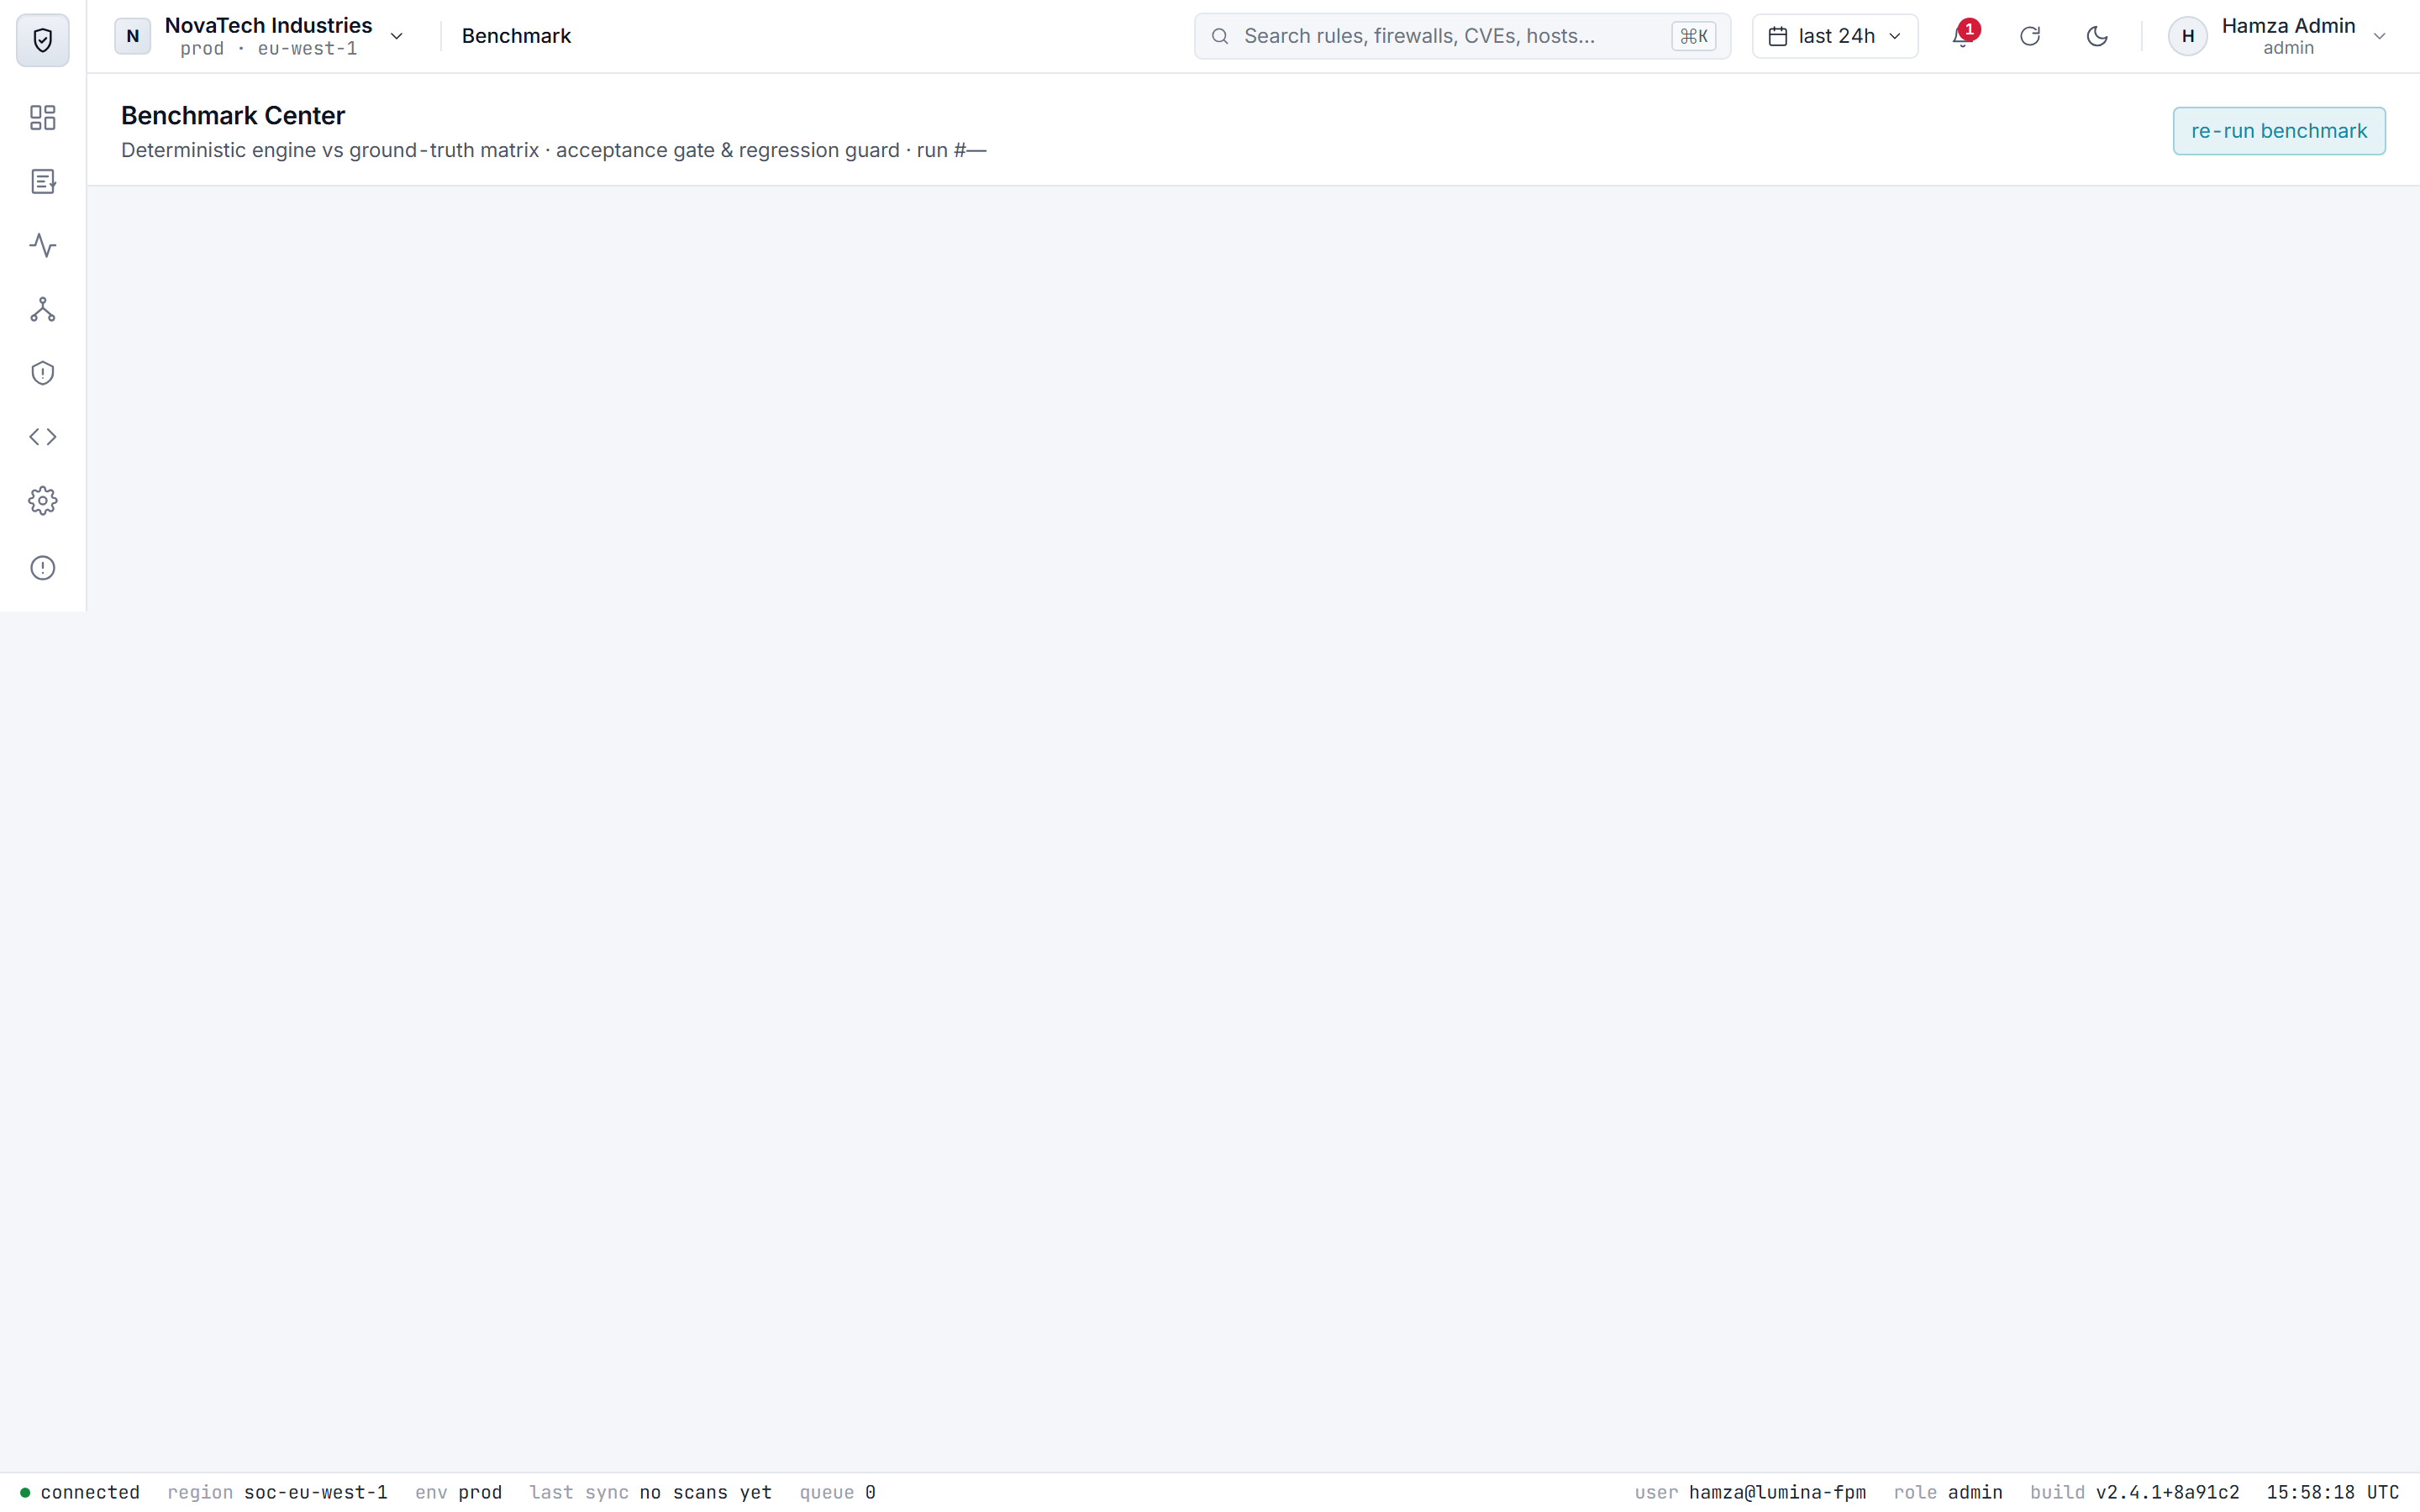
\includegraphics[width=0.97\linewidth]{figures/ui-benchmark.png}}
\caption{LuminaFPM benchmark center (acceptance gate).}\label{fig:ui-benchmark}
\end{figure}

The Benchmark Center screen (\path{frontend/src/benchmark.tsx}, Figure~\ref{fig:ui-benchmark}) renders this scorecard as live tiles --- precision, recall, $F_1$, and severity-match --- alongside the TP/FP/FN/cases summary, a coverage-by-anomaly-type table, and a per-case matrix. On run~\#25 every tile reads 100\%, the summary reads 43/0/0/43, and each of the 43 per-case rows is an exact match. It is important to be precise about what this scorecard certifies: \emph{within the config-only taxonomy bucket and the deployed lab policy set}, the engine detects every expected anomaly, raises no spurious ones, and assigns the correct severity. It does \emph{not} claim coverage of the full 46-type taxonomy --- the not-yet-implemented and telemetry-dependent types are deliberately out of this bucket (Section~\ref{sec:ch4-findings}).

\subsection{CTI test case}
\label{sec:ch4-cti-case}

The CTI subsystem was validated end-to-end with the deterministic, network-free \texttt{LabOfflineProvider}, whose \texttt{KNOWN\_BAD} table maps the indicator \texttt{185.220.101.1} (a long-standing Tor exit / abuse source) to a verdict of \emph{malicious}, threat type \texttt{tor\_exit}, severity \emph{high}, confidence~0.85. Two rules permit traffic to this indicator: \texttt{FGT\_ANY\_DB} (whose database-object set resolves to include the indicator) and the deliberately config-clean demonstrator \texttt{PA\_ALLOW\_MALICIOUS}. The CTI runner extracted the indicator, enriched it, and correlated it across \emph{all} devices' objects, raising a \texttt{threat\_exposure} finding (\texttt{detection\_mode="cti"}) on each of those allow rules --- one per device. The test also confirmed the platform's data-minimization guarantee: \texttt{internal\_indicators\_sent} was \texttt{false}, i.e.\ the RFC1918 lab objects were never transmitted to any external provider. Because \texttt{threat\_exposure} is a cti-mode finding rather than a config anomaly, it is excluded from the config-only benchmark scorecard above while still feeding the risk recalculation, which lifted the affected FortiGate rule's risk through an added \texttt{cti} factor (+28).

\begin{figure}[htbp]
\centering
\fbox{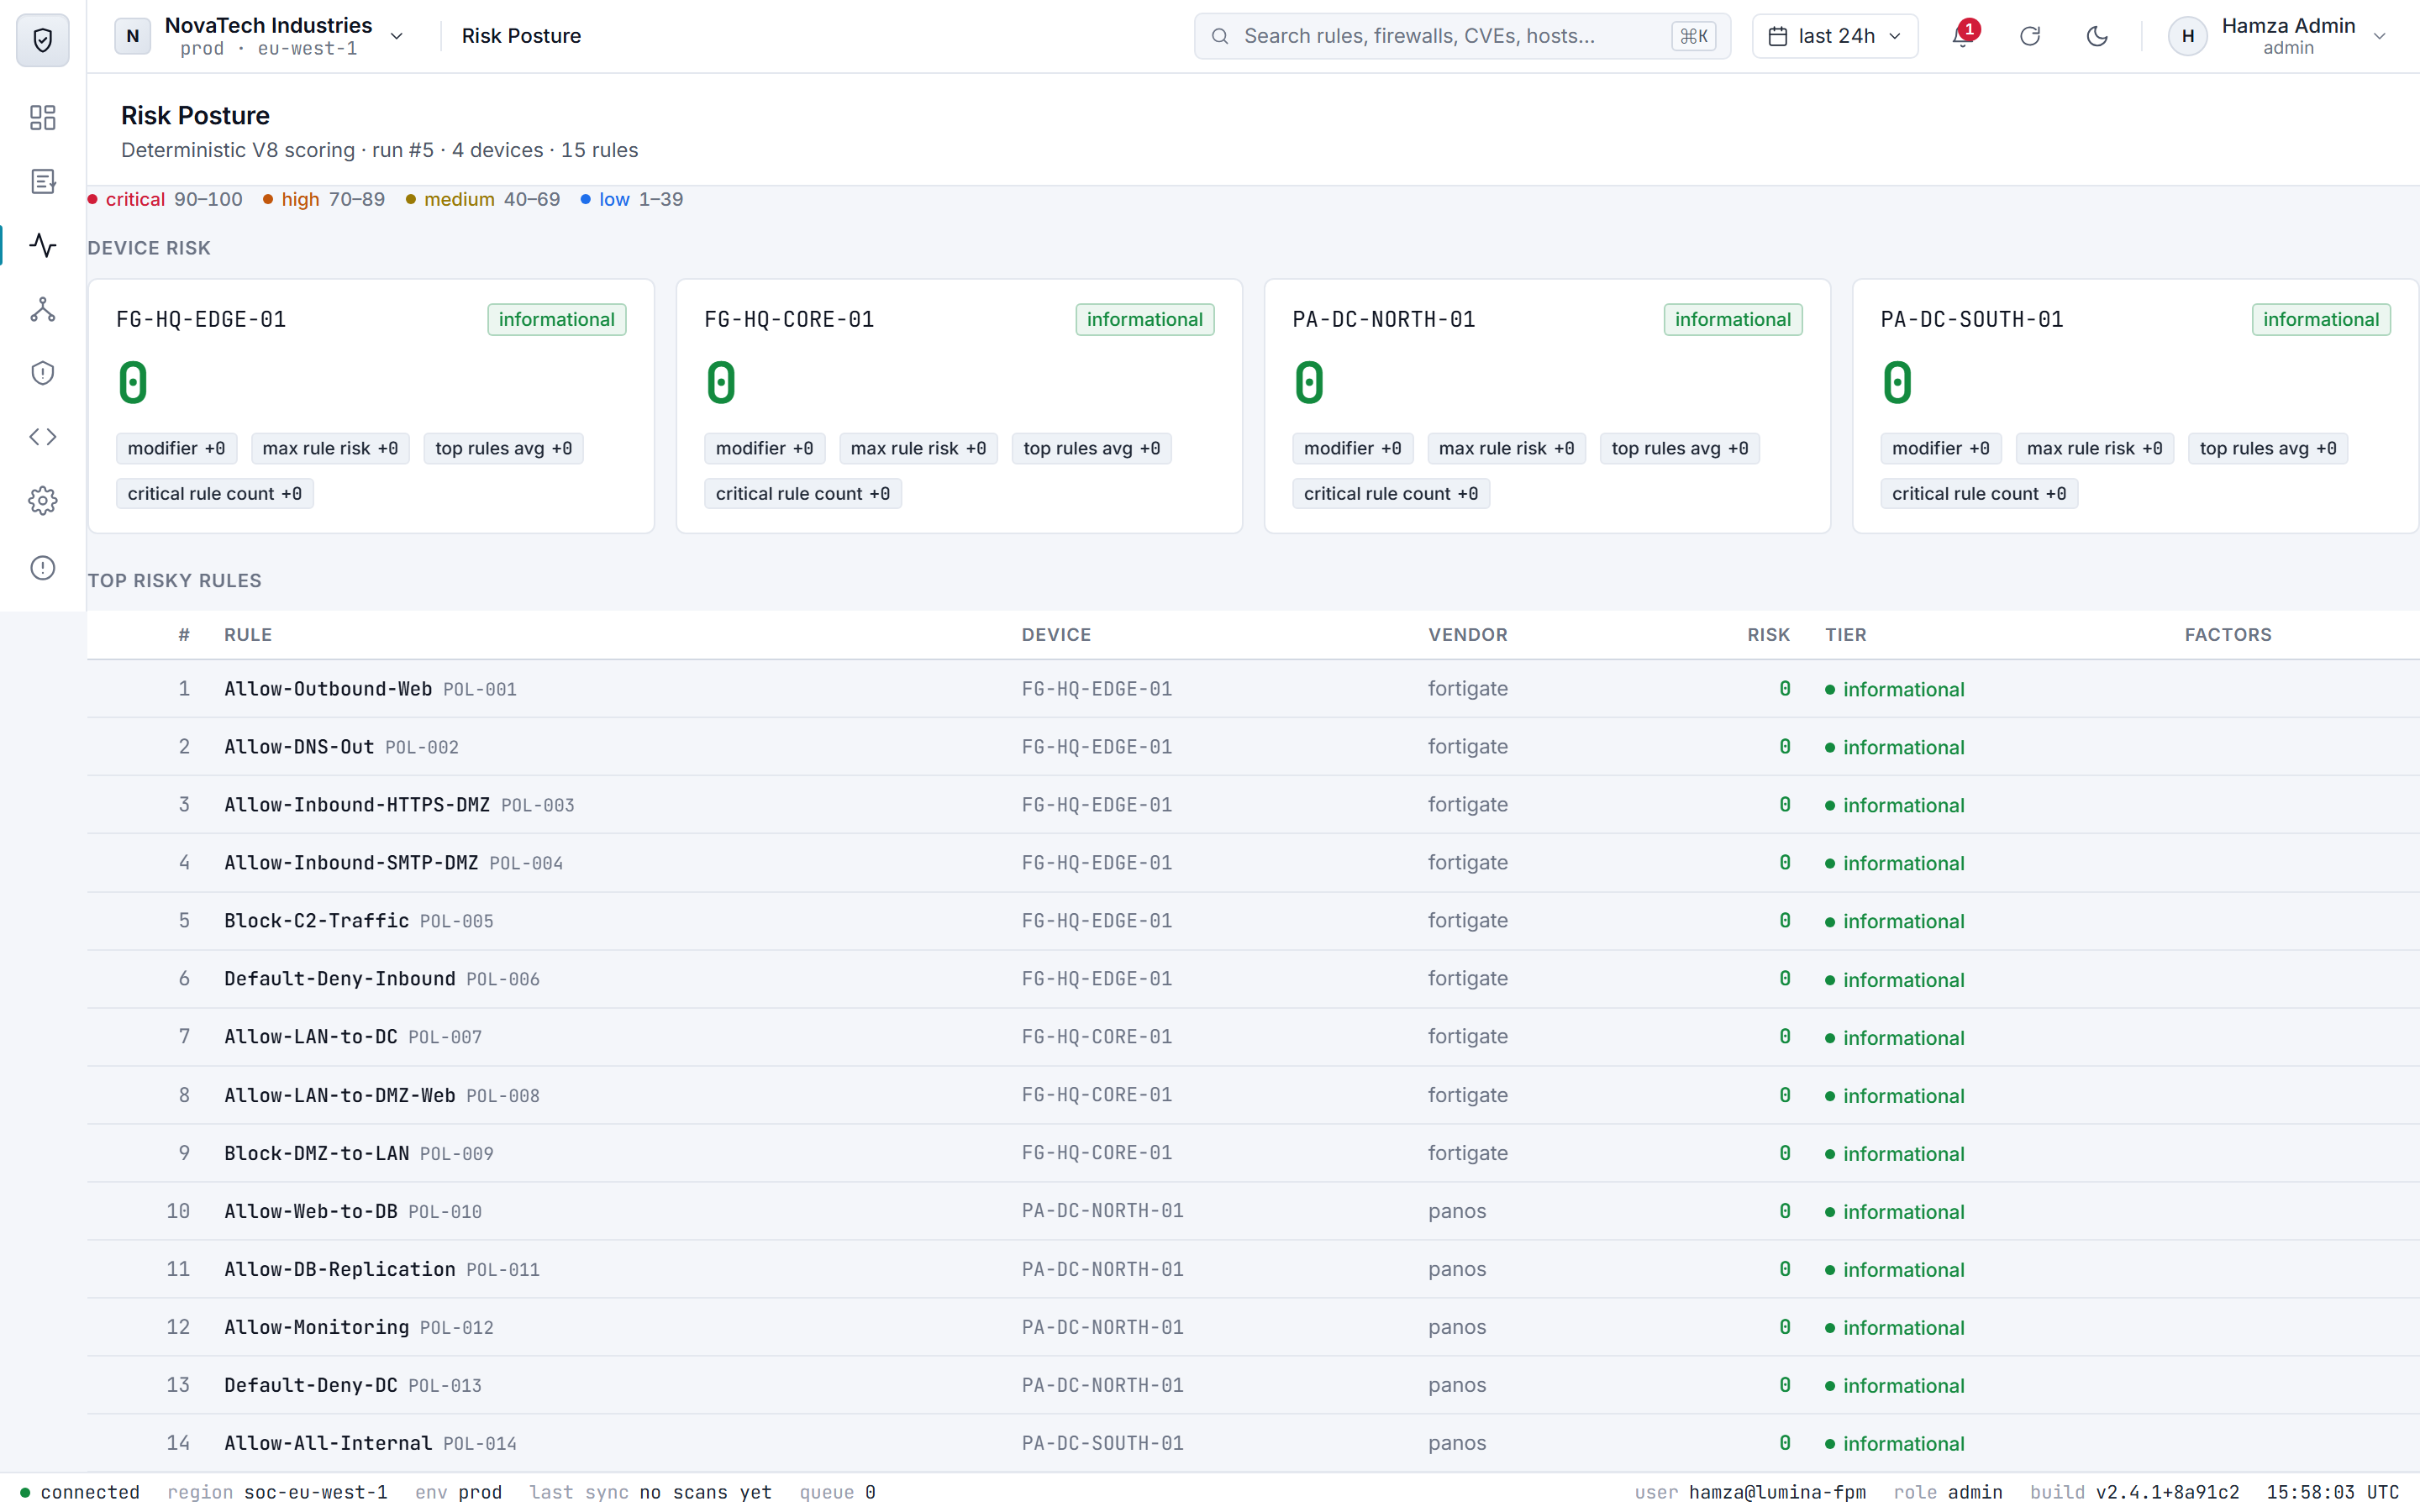
\includegraphics[width=0.97\linewidth]{figures/ui-risk.png}}
\caption{LuminaFPM risk posture screen.}\label{fig:ui-risk}
\end{figure}

The Risk Posture screen (\path{frontend/src/risk.tsx}, Figure~\ref{fig:ui-risk}) renders per-device risk cards and a top-risky-rules table with \texttt{factor\_breakdown} chips and the tier legend. On run~\#25 both the PA-LAB and FGT-LAB cards reach the critical ceiling of~100 (FortiGate's rule-blend base of~96 is lifted to~100 by its firmware-CVE device modifier), with \texttt{PA\_ANY\_DB}/\texttt{FGT\_ANY\_DB} at~99 and \texttt{FGT\_ANY\_ANY}/\texttt{PA\_ANY\_ANY} at~98, each carrying its per-rule factor breakdown (anomaly, exposure, posture, logging, asset-sensitivity). That breakdown is the audit trail that explains \emph{why} a rule scored as it did.

\subsection{AI-report test case}

The LLM SOC-reporting path was validated for a rule-scoped report on \texttt{FGT\_ANY\_DB}. The reporter assembled that rule's four deterministic findings, its risk assessment, and the CTI observation, embedding their database IDs as \texttt{evidence\_refs}: \texttt{\{anomaly\_ids:[391,410,424,440], risk\_id:243, cti\_observation\_ids:[4]\}}. With a valid key, \texttt{gemini-2.5-flash} produced a polished SOC report that cited each evidence ID, attributed the CTI verdict explicitly to the \texttt{lab\_offline} provider, labelled its prose as ``Analysis'', and invented nothing --- demonstrating the Volume~10 guardrail that \emph{the deterministic engine, not the LLM, decides what is an anomaly; the LLM explains and prioritizes}. The same test also exercised the graceful-failure path: when an earlier key returned \texttt{API\_KEY\_INVALID}, the platform fell back to the deterministic \texttt{OfflineProvider}, which renders the same grounded evidence verbatim under an explicit ``not an AI analysis'' header, and the report was still persisted with \texttt{status} recorded. This proves the platform always reports, with or without a working LLM, and never lets the AI layer fabricate a finding.

\section{Findings and Limitations}
\label{sec:ch4-findings}

The evaluation establishes that LuminaFPM's core thesis holds: a strictly read-only platform can acquire multi-vendor firewall policy, normalize it into a single canonical model, and detect cross-vendor anomalies deterministically with measurable, perfect precision and recall against ground truth on the lab policy set. In the spirit of honest academic reporting, the following limitations bound that claim and define the scope of future work.

\begin{itemize}[leftmargin=1.4em]
  \item \textbf{Config-detectable subset, not the full taxonomy.} v1 ships 14 deterministic detectors (plus the cti-mode \texttt{threat\_exposure}), covering the config-only core of the 46-type taxonomy (shadowing, redundancy, conflict, permissiveness, posture, sensitivity, cross-device). The remaining $\sim$32 types --- firewall-specific (zone mismatch, NAT risk, weak profile, direction), lifecycle/history (drift, age, rule explosion, change frequency), and runtime/advanced (hit distribution, time-of-day, geo, compliance, asymmetric) --- are \emph{specified but not implemented}, because they require hit-counts, history, or enterprise telemetry that the config-only pipeline does not ingest. The perfect benchmark scorecard certifies the config-only bucket only.
  \item \textbf{Benchmark gate is reported, not enforced in CI.} The runner computes and exposes the metrics, but no automated pass/fail threshold is wired into a build or CI pipeline; acceptance is currently a qualitative human gate against Volume~7 Table~7.
  \item \textbf{Topology depicts logical intent, not traffic.} The topology view has been rebuilt as an interactive Cytoscape.js graph (draggable nodes with a layout persisted to \texttt{localStorage}, zoom/pan, a live firmware-CVE badge, and PNG export). By design it depicts the \emph{configured} logical relationships derived from policy and asset context, not runtime packet flow, NetFlow, or sessions --- a deliberate architectural boundary rather than a limitation of the renderer.
  \item \textbf{Cosmetic login.} The frontend retains a cosmetic lab login gate; the backend exposes no authentication route in v1, so the login does not enforce real access control and is an intentional placeholder.
  \item \textbf{FortiGate-VM constraints.} The unlicensed FortiGate VM imposes a ten-policy cap, which forced trade-offs in the deployed FortiGate set (a disabled-rule case and an object-sprawl case could not both be fitted under the cap), so \texttt{object\_sprawl} is implemented but not exercised by this small lab set; \texttt{disabled\_rule\_review} \emph{is} exercised, on the Palo Alto side, via \texttt{PA\_DISABLED\_RISKY}. The same VM's admin HTTPS listener could not negotiate a usable TLS cipher, requiring a lab-only, explicitly-allow-listed HTTP escape hatch (\texttt{FIREWALL\_INSECURE\_HTTP\_HOSTS}); production remains HTTPS-only.
  \item \textbf{Lab, not production.} All live results are from a parallel two-device VMware lab on a thin, purpose-built policy set. The numbers demonstrate correctness on a controlled ground truth; they are not a statement about behaviour or scale on a large production estate, and the dark-web LTI subsystem remains optional and off by default.
\end{itemize}

A notable diagnostic outcome, reported here as evidence of the strategy's value, is the FortiGate \texttt{ALL}-service defect: an early live run revealed that FortiGate \texttt{shadowing}/\texttt{redundancy} did not fire while the identical Palo Alto designs did. Investigation traced this to FortiGate's predefined \texttt{ALL} service normalizing to \texttt{unknown:any} rather than the canonical ANY-service sentinel, so superset-based detectors missed it while the overlap-based \texttt{conflict} detector masked the bug by still firing. The fix --- mapping \texttt{ALL}/\texttt{any} to the canonical ANY service in normalization --- raised the run's findings from 38 to 46 and was permanently captured as a normalization regression test. This is precisely the layered strategy working as intended: a defect surfaced by live validation, root-caused, fixed, and locked down at the unit-test layer so it can never silently recur.

Relevant source files: \path{backend/services/benchmark/scorer.py}, \path{backend/services/benchmark/ground_truth.py}, \path{backend/services/benchmark/runner.py}, \path{backend/tests/test_*.py}, \path{frontend/src/benchmark.tsx}, \path{frontend/src/risk.tsx}.

\chapter{Conclusion and Future Work}
\label{sec:ch5-intro}

This final chapter draws the project to a close. Section~\ref{sec:ch5-conclusion} consolidates what \textsc{LuminaFPM} achieved against the objectives that motivated it, summarising the read-only multi-vendor pipeline, the deterministic set-theoretic detection engine, and the empirical validation obtained on the live laboratory. Section~\ref{sec:ch5-future} then sets out a concrete, grounded roadmap of enhancements that follow naturally from the v1 architecture, distinguishing engineering hardening from genuine capability extensions.

\section{Conclusion}
\label{sec:ch5-conclusion}

The goal of this project was to design and build a vendor-neutral platform that could read firewall policy from heterogeneous devices, reason about that policy in a single unified model, and surface the latent anomalies --- shadowing, redundancy, correlation, generalisation, and cross-device inconsistency --- that accumulate silently in production rule bases and that human operators are poorly equipped to find by manual inspection. \textsc{LuminaFPM} delivers that platform as a working, integrated system rather than a paper design.

\subsection{What was achieved}
\label{sec:ch5-achieved}

The central engineering claim of this work is realised end to end. \textsc{LuminaFPM} acquires firewall configuration from two distinct vendors --- Fortinet FortiGate over the FortiOS REST/JSON API and Palo Alto Networks PAN-OS over the XML-API --- through a strictly \emph{read-only} connector layer (\texttt{ConnectorInterface}, with \texttt{FortiGateConnector} and \texttt{PaloAltoConnector} implementations) that issues only \texttt{GET}-equivalent retrieval calls and never writes, pushes, or commits to a device. This read-only guarantee is not merely a policy statement: it is enforced structurally in the connector contract and is preserved through every downstream layer, so the platform can be deployed against live production firewalls without any risk of altering their posture.

Acquired policy from these dissimilar vendors is then \emph{normalised} into a single canonical model persisted in PostgreSQL, which serves as the system's source of truth. The normalisation layer correlates heterogeneous network and service objects across vendors --- recording each correspondence in \texttt{object\_normalization\_mapping} with an explicit \texttt{match\_method} (for example \texttt{exact\_name\_value}, \texttt{exact\_value}, or \texttt{name\_similarity}) and a numeric confidence --- so that a FortiGate address object and an equivalent PAN-OS address object are reasoned about as one logical entity. This normalisation is the foundation that makes genuine cross-vendor analysis possible, including the detection of cross-device inconsistencies that no single-vendor tool can express.

On top of the normalised model runs the project's analytical core: a \emph{deterministic} anomaly-detection engine. The engine is best understood through the set-theory framing developed in the earlier chapters --- each rule is treated as a tuple of sets over source, destination, service, and action, with shadowing expressed as a subset/superset relation, redundancy as set equivalence, and conflict as overlapping match with differing action --- but its implementation is a transparent, rule-based engine over the unified model, not a machine-learning classifier. Determinism is a deliberate and load-bearing design decision: every finding is reproducible, explainable, and traceable to the exact pair of rules and the exact set relation that produced it. In v1 this engine ships its ``config-only core'' --- fourteen detectors in \texttt{ALL\_DETECTORS} emitting fourteen distinct \texttt{anomaly\_type} values --- which together with the CTI-derived \texttt{threat\_exposure} type yields fifteen persisted anomaly classes drawn from the broader forty-six-category taxonomy.

Around this deterministic spine the platform layers three further capabilities that turn raw findings into operator-actionable intelligence. A deterministic \emph{risk-scoring} subsystem (\texttt{RISK\_VERSION} \texttt{1.0.0}) assigns each finding and each device a bounded $0$--$100$ score from a fixed, auditable formula combining anomaly severity, exposure, asset sensitivity, security posture, logging, cross-vendor weight, CTI signal, and lifecycle factors, and assigns tier bands so that operators can triage by priority. An API-based \emph{cyber threat intelligence} layer correlates policy exposure against external indicators. Finally, an \emph{AI-assisted reporting} layer generates SOC-oriented and executive reports through an LLM provider abstraction (\texttt{GeminiProvider} as the documented default, with a deterministic, network-free \texttt{OfflineProvider} fallback). Crucially, the LLM is never an anomaly authority: it ``explains, never detects.'' Every generated report is \emph{evidence-grounded}, carrying explicit \texttt{evidence\_refs} that point back to the database identifiers of the deterministic findings it describes, so that no claim in a report exists without a verifiable, machine-checked basis in the engine's output. This separation --- deterministic engine as the source of truth, LLM as a bounded narrator --- is what makes \textsc{LuminaFPM}'s AI output trustworthy in a security context.

Beyond the originally scoped plan, the delivered system carries several further capabilities that proved valuable in practice. The threat-intelligence layer gained a second, \emph{firmware-CVE device-vulnerability} axis: a device's reported firmware version is correlated against a curated CVE reference (including CISA-KEV-listed entries), raising a device-scope risk modifier without emitting any rule-level findings, so the vulnerability signal sharpens device prioritisation while leaving the benchmarked detection corpus untouched. The reporting layer is underpinned by a \emph{deterministic, structured report builder} --- pure database assembly that produces the prioritised-remediation, risk-posture, firmware-vulnerability, and per-finding-evidence tables independently of the LLM --- with the assembled report exportable as GitHub-flavoured Markdown and as a browser-rendered PDF. Finally, the platform ships a functional \emph{Settings console} that exposes device management, scheduled (Celery Beat) acquisition, detection, and threat-intelligence jobs, and in-app notifications emitted from the pipeline, turning the system from a one-shot analysis tool into a continuously operable platform.

\begin{figure}[htbp]
\centering
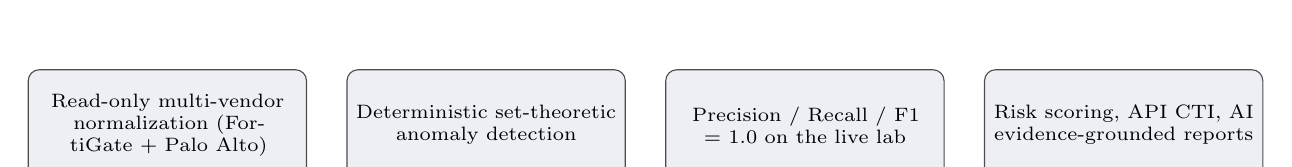
\begin{tikzpicture}[
  ach/.style={draw=black!70, rounded corners, fill=LightGray, text width=3.3cm, align=center, minimum height=14mm, font=\scriptsize},
  node distance=5mm]
\node[ach] (a) {Read-only multi-vendor normalization (FortiGate + Palo Alto)};
\node[ach, right=of a] (b) {Deterministic set-theoretic anomaly detection};
\node[ach, right=of b] (c) {Precision / Recall / F1 = 1.0 on the live lab};
\node[ach, right=of c] (d) {Risk scoring, API CTI, AI evidence-grounded reports};
\end{tikzpicture}
\caption{Summary of the principal achievements delivered by LuminaFPM.}
\label{fig:ch5-achievement-summary}
\end{figure}

\subsection{Empirical validation}
\label{sec:ch5-validation}

The system's correctness was not asserted but measured. A dedicated benchmark subsystem (\texttt{services/benchmark/} comprising \texttt{ground\_truth.py}, \texttt{scorer.py}, and \texttt{runner.py}, surfaced through \texttt{/api/v1/benchmark}) scores the live engine output against a hand-curated ground-truth matrix at \emph{(rule, anomaly\_type)} granularity, computing true positives, false positives, false negatives, and the standard information-retrieval metrics precision $=\text{TP}/(\text{TP}+\text{FP})$, recall $=\text{TP}/(\text{TP}+\text{FN})$, and $F_1 = 2PR/(P+R)$, together with a severity-match rate.

Run against the parallel VMware laboratory --- a live FortiGate (\texttt{192.168.55.10}) and a live Palo Alto (\texttt{192.168.55.20}) on the shared \texttt{192.168.55.0/24} network --- the platform read-synced both devices, executed an all-scope detection run, and analysed \textbf{26 active rules across 2 devices} (10 on FortiGate and 16 on Palo Alto). Scored against the ground truth, the deterministic engine achieved \textbf{precision, recall, and $F_1$ all equal to $1.0$}, with \textbf{43 true positives, zero false positives, and zero false negatives} (43 of 43 expected cases matched) and a \textbf{severity-match rate of $1.0$}. This is the project's headline result: on the validated laboratory corpus the engine detected every anomaly it was expected to detect, assigned the correct severity in every case, and reported no spurious findings, confirming both the soundness of the set-theoretic model and the fidelity of its deterministic implementation. Because the benchmark is wired as a first-class, re-runnable acceptance gate in both the API and the user interface (the Benchmark Center), this result functions as a standing regression guard rather than a one-off measurement.

In summary, \textsc{LuminaFPM} meets its objectives: it is a strictly read-only, multi-vendor firewall anomaly-management platform whose normalised model and deterministic, explainable engine were validated at perfect precision, recall, and $F_1$ on a live two-vendor laboratory, and whose risk-scoring, threat-intelligence, and evidence-grounded AI-reporting layers translate findings into intelligence a security operations team can act on with confidence.

\section{Future Work}
\label{sec:ch5-future}

The v1 system is complete and validated within its declared scope, and that scope was deliberately bounded to guarantee a working, defensible deliverable. The following enhancements are the natural next steps; they are grouped into capability extensions, security/operational hardening, and platform breadth. Each is grounded in a concrete gap or seam already present in the codebase.

\subsection{Interactive logical topology on Cytoscape.js}
\label{sec:ch5-cytoscape}

The topology view has been rebuilt as a true interactive graph on Cytoscape.js, replacing the earlier hand-rolled static SVG layout. It renders the same real platform data --- firewalls, zones, monitored assets, and CTI threat vectors --- now as draggable nodes whose positions persist across sessions (in browser local storage), with zoom and pan, a live firmware-CVE badge sourced from each device's acquired firmware version, and PNG export of the current view. The graph continues to depict \emph{logical policy intent} --- the relationships configured in policy --- and never live packet forwarding, NetFlow, sessions, or deep packet inspection; that distinction is architectural and remains explicit in the user interface. The residual work is therefore polish rather than rebuild: wiring an automatic directed layout (Dagre) as an alternative to the persisted manual arrangement, and adding expand/collapse with focus traversal over larger estates.

\subsection{Real authentication and RBAC enforcement}
\label{sec:ch5-rbac}

The security model specifies five read-centric roles, and a demonstration security-key login exists at the UI layer, but the API route handlers themselves currently carry no authorisation dependency --- \texttt{get\_db\_session} is the only \texttt{Depends} on the reviewed routers, so per-endpoint authorization is not yet enforced in code. A priority hardening task is therefore to implement real authentication (session or token based) and to wire genuine role-based access control as a route-level dependency across every endpoint, so that the documented five-role model is enforced rather than merely described. This is a prerequisite for any multi-tenant or production deployment.

\subsection{Broadening the deterministic engine to the full taxonomy}
\label{sec:ch5-taxonomy}

v1 implements the fourteen-detector config-only core out of the specified forty-six-category taxonomy. A substantial body of future work is to implement the remaining specified-but-unimplemented categories --- for example ordering anomalies, temporary-rule decay, poor-naming hygiene, zone mismatch, NAT risk, and asymmetric-rule detection. A particularly valuable subset is the \emph{conditional} and \emph{telemetry/history-based} categories, which depend on signals beyond static configuration. Extending the engine to these would require carefully introduced, optional data sources while preserving the determinism and full explainability that are the engine's defining strengths: any history-aware detector must still emit reproducible findings traceable to concrete evidence.

\subsection{Activating the threat-intelligence and dark-web module}
\label{sec:ch5-lti}

The cyber threat-intelligence layer is delivered and active by default across two axes. The \emph{indicator} axis correlates policy exposure against external indicators of compromise --- shipping an offline indicator set so it operates without network access, with an optional keyed online provider --- and the \emph{firmware-CVE} axis correlates each device's firmware version against a curated CVE reference, both feeding the risk score under deterministic control. What remains genuinely future is the dark-web / OSINT subsystem (the LTI/Robin curation layer and its richer LLM model-routing): it exists in the codebase but is off by default and treated as optional. Maturing it --- enabling its curated clear-net and dark-web feeds, validating their correlation against the deterministic findings, and integrating that output into the risk score and reports under explicit operator control --- would extend \textsc{LuminaFPM} from policy-posture analysis toward proactive, externally-informed exposure assessment. As with the LLM reporter, any such integration must keep the deterministic engine as the authority and the threat-intel layer as an evidence-grounded enrichment, never an unverifiable signal.

\subsection{Additional vendors}
\label{sec:ch5-vendors}

v1 supports FortiGate and Palo Alto only; Cisco was explicitly de-scoped (ADR-004), and the connector registry contains no Cisco connector. Because the architecture cleanly separates vendor-specific acquisition (the \texttt{ConnectorInterface} contract) from the vendor-neutral normalised model and engine, adding a vendor is principally a matter of writing a new read-only connector and its normalisation mapping. Cisco (for example ASA/Firepower) is the obvious first candidate for a future release; the platform's normalisation and detection layers would absorb a third vendor without modification, and would immediately gain the ability to detect Cisco-versus-Fortinet and Cisco-versus-Palo-Alto cross-device inconsistencies. (Any residual Cisco/ASA strings remaining in demo seed data and UI styling should be removed until a real connector exists, to avoid implying unsupported capability.)

\subsection{Report export to PDF}
\label{sec:ch5-pdf}

Direct export of the evidence-grounded reports has been delivered. The platform now exports each generated SOC and executive report both as GitHub-flavoured Markdown (served directly from the API) and as a self-contained PDF produced through the browser's print pipeline, yielding a distributable artefact suitable for audit trails, management reporting, and compliance evidence. The underlying \texttt{evidence\_refs} linkage is preserved through the export, so every exported claim remains traceable to the deterministic finding that produced it. The residual future work is purely presentational: a richer, server-side native PDF renderer with bespoke typographic styling, should fully controlled print layout become a requirement.

\subsection{Operator-supplied topology and asset context}
\label{sec:ch5-topology-input}

In v1 the platform derives logical relationships, zones, and monitored assets purely from \emph{configured intent} in the acquired policy; there is no ingestion path for an external or observed topology. A valuable enhancement is an explicit operator-supplied topology/asset input --- allowing an operator to declare zones, asset sensitivity, and business context --- which would sharpen risk scoring (asset sensitivity in particular) and enrich the logical graph. This would remain a description of intended/declared structure, consistent with the platform's principle of reasoning over configured posture rather than observed traffic.

\subsection{Production hardening}
\label{sec:ch5-hardening}

Finally, several engineering tasks separate the validated laboratory build from a production deployment: removing declared-but-unused frontend dependencies and dead vendor code paths; pinning and auditing dependency versions; tightening secret and encryption-key management; expanding automated test and CI coverage around the connectors and engine; production-grade observability and structured logging; and hardening the Docker Compose deployment for resilient, secured operation. None of these alters the core architecture; together they raise the system from a demonstrably-correct prototype to a deployable product.

\begin{figure}[htbp]
\centering
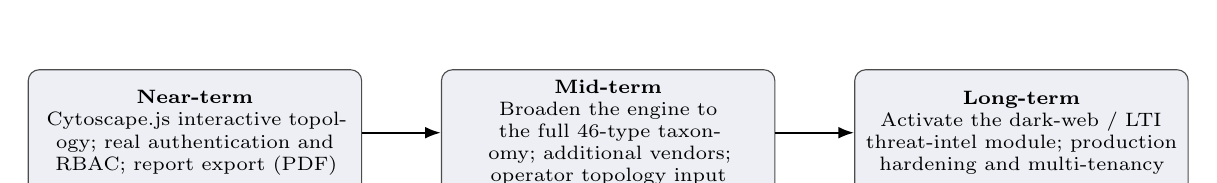
\begin{tikzpicture}[
  ph/.style={draw=black!70, rounded corners, fill=LightGray, text width=4.0cm, align=center, minimum height=16mm, font=\scriptsize},
  flow/.style={-{Latex[length=2mm]}, thick}, node distance=10mm]
\node[ph] (p1) {\textbf{Near-term}\\Cytoscape.js interactive topology; real authentication and RBAC; report export (PDF)};
\node[ph, right=of p1] (p2) {\textbf{Mid-term}\\Broaden the engine to the full 46-type taxonomy; additional vendors; operator topology input};
\node[ph, right=of p2] (p3) {\textbf{Long-term}\\Activate the dark-web / LTI threat-intel module; production hardening and multi-tenancy};
\draw[flow] (p1) -- (p2);
\draw[flow] (p2) -- (p3);
\end{tikzpicture}
\caption{Future-work roadmap for LuminaFPM.}
\label{fig:ch5-future-roadmap}
\end{figure}

Taken together, these directions extend \textsc{LuminaFPM} along three axes --- deeper analysis (full taxonomy, threat-intel), broader coverage (more vendors, richer topology input), and production readiness (RBAC, hardening, PDF export) --- while preserving the two principles that define the platform: it remains strictly read-only with respect to the firewalls it analyses, and its findings remain deterministic, explainable, and evidence-grounded.

\cleardoublepage
\addcontentsline{toc}{chapter}{References}
%
\begin{thebibliography}{99}

\bibitem{alshaer2004}
E.~S. Al-Shaer and H.~H. Hamed, ``Discovery of policy anomalies in distributed firewalls,'' in \emph{Proc. IEEE INFOCOM 2004}, vol.~4, Hong Kong, 2004, pp.~2605--2616.

\bibitem{alshaer2005taxonomy}
E.~S. Al-Shaer, H.~H. Hamed, R.~Boutaba, and M.~Hasan, ``Conflict classification and analysis of distributed firewall policies,'' \emph{IEEE Journal on Selected Areas in Communications}, vol.~23, no.~10, pp.~2069--2084, Oct.~2005.

\bibitem{hamed2006taxonomy}
H.~Hamed and E.~Al-Shaer, ``Taxonomy of conflicts in network security policies,'' \emph{IEEE Communications Magazine}, vol.~44, no.~3, pp.~134--141, Mar.~2006.

\bibitem{yuan2006fireman}
L.~Yuan, J.~Mai, Z.~Su, H.~Chen, C.-N. Chuah, and P.~Mohapatra, ``FIREMAN: A toolkit for firewall modeling and analysis,'' in \emph{Proc. IEEE Symp. Security and Privacy (S\&P)}, Oakland, CA, USA, 2006, pp.~199--213.

\bibitem{wool2004quantitative}
A.~Wool, ``A quantitative study of firewall configuration errors,'' \emph{IEEE Computer}, vol.~37, no.~6, pp.~62--67, Jun.~2004.

\bibitem{gouda2007structured}
M.~G. Gouda and A.~X. Liu, ``Structured firewall design,'' \emph{Computer Networks}, vol.~51, no.~4, pp.~1106--1120, Mar.~2007.

\bibitem{fortinet_restapi}
Fortinet, Inc., \emph{FortiOS REST API Reference and Administration Guide}. [Online]. Available: \url{https://docs.fortinet.com/document/fortigate/}. [Accessed: Jun.~2026].

\bibitem{paloalto_xmlapi}
Palo Alto Networks, Inc., \emph{PAN-OS XML API Usage Guide}. [Online]. Available: \url{https://docs.paloaltonetworks.com/pan-os/pan-os-panorama-api}. [Accessed: Jun.~2026].

\bibitem{paloalto_panorama}
Palo Alto Networks, Inc., \emph{Panorama Administrator's Guide: Centralized Firewall Policy Management}. [Online]. Available: \url{https://docs.paloaltonetworks.com/panorama}. [Accessed: Jun.~2026].

\bibitem{tufin}
Tufin Software Technologies, \emph{Tufin Orchestration Suite: Firewall Policy and Security Change Automation}. [Online]. Available: \url{https://www.tufin.com/}. [Accessed: Jun.~2026].

\bibitem{algosec}
AlgoSec, Inc., \emph{AlgoSec Security Management Solution: Firewall Policy Analysis and Optimization}. [Online]. Available: \url{https://www.algosec.com/}. [Accessed: Jun.~2026].

\bibitem{firemon}
FireMon, LLC, \emph{FireMon Security Manager: Firewall Rule Analysis and Compliance}. [Online]. Available: \url{https://www.firemon.com/}. [Accessed: Jun.~2026].

\bibitem{skybox}
Skybox Security, Inc., \emph{Skybox Security Posture Management Platform: Firewall Assurance}. [Online]. Available: \url{https://www.skyboxsecurity.com/}. [Accessed: Jun.~2026].

\bibitem{nvd}
National Institute of Standards and Technology (NIST), \emph{National Vulnerability Database (NVD)}. [Online]. Available: \url{https://nvd.nist.gov/}. [Accessed: Jun.~2026].

\bibitem{cisa_kev}
Cybersecurity and Infrastructure Security Agency (CISA), \emph{Known Exploited Vulnerabilities (KEV) Catalog}. [Online]. Available: \url{https://www.cisa.gov/known-exploited-vulnerabilities-catalog}. [Accessed: Jun.~2026].

\bibitem{mitre_attack}
The MITRE Corporation, \emph{MITRE ATT\&CK: Adversarial Tactics, Techniques, and Common Knowledge}. [Online]. Available: \url{https://attack.mitre.org/}. [Accessed: Jun.~2026].

\bibitem{abuseipdb}
AbuseIPDB, \emph{AbuseIPDB IP Address Reputation and Abuse Reporting API (v2)}. [Online]. Available: \url{https://www.abuseipdb.com/}. [Accessed: Jun.~2026].

\bibitem{fastapi}
S.~Ram\'irez, \emph{FastAPI: Modern, Fast (High-Performance) Web Framework for Building APIs with Python}. [Online]. Available: \url{https://fastapi.tiangolo.com/}. [Accessed: Jun.~2026].

\bibitem{sqlalchemy}
M.~Bayer, \emph{SQLAlchemy: The Python SQL Toolkit and Object Relational Mapper}. [Online]. Available: \url{https://www.sqlalchemy.org/}. [Accessed: Jun.~2026].

\bibitem{celery}
A.~Solem and the Celery Team, \emph{Celery: Distributed Task Queue}. [Online]. Available: \url{https://docs.celeryq.dev/}. [Accessed: Jun.~2026].

\bibitem{postgresql}
The PostgreSQL Global Development Group, \emph{PostgreSQL: The World's Most Advanced Open Source Relational Database}. [Online]. Available: \url{https://www.postgresql.org/docs/}. [Accessed: Jun.~2026].

\bibitem{react}
Meta Open Source, \emph{React: A JavaScript Library for Building User Interfaces}. [Online]. Available: \url{https://react.dev/}. [Accessed: Jun.~2026].

\bibitem{docker}
Docker, Inc., \emph{Docker Compose: Define and Run Multi-Container Applications}. [Online]. Available: \url{https://docs.docker.com/compose/}. [Accessed: Jun.~2026].

\bibitem{gemini}
Google LLC, \emph{Gemini API Documentation (Google Generative AI)}. [Online]. Available: \url{https://ai.google.dev/}. [Accessed: Jun.~2026].

\bibitem{rfc1918}
Y.~Rekhter, B.~Moskowitz, D.~Karrenberg, G.~J. de~Groot, and E.~Lear, ``Address allocation for private internets,'' RFC~1918, Internet Engineering Task Force (IETF), Feb.~1996.

\end{thebibliography}

\end{document}
